% !TeX root = ../../../main.tex
\section{Preventivo} \label{_preventivo}
In questa sezione viene riportato il preventivo per il progetto, suddividendo le ore di lavoro e i costi nelle varie fasi descritte in dettaglio in \S\ref{_pianificazione}.
Le fasi di analisi e di consolidamento dei requisiti, tuttavia, non vengono tenute in considerazione nel calcolo del preventivo finale.
La suddivisione oraria dei ruoli per ogni membro del gruppo dovrà rispettare le seguenti regole:
\begin{itemize}
	\item ogni componente dovrà ricoprire almeno una volta ogni ruolo per almeno otto ore, in modo che tutti i componenti apprendano le attività e le responsabilità legate ai diversi ruoli;
	\item le ore lavorative per ogni fase dovranno essere le stesse per ogni componente, per far si che tutti apportino lo stesso contributo al progetto, senza alcuna differenza.
\end{itemize}
Per riportare i ruoli nelle tabelle, essi sono abbreviati con le seguenti sigle:
\begin{itemize}
	\item\textbf{Re:} responsabile;
	\item\textbf{Am:} amministratore;
	\item\textbf{An:} analista;
	\item\textbf{Pg:} progettista;
	\item\textbf{Pr:} programmatore;
	\item\textbf{Ve:} verificatore.
\end{itemize}

\subsection{Fase di analisi dei requisiti}

\paragraph{Prospetto orario}
Durante la fase di analisi dei requisiti la distribuzione oraria complessiva sarà la seguente:

\rowcolors{1}{lightest-grayest}{blue!20}
\begin{longtable}{|l|c|c|c|c|c|c|c|}
	\hline
	\rowcolor{lighter-grayer}
	\textbf{Nome}     & \textbf{Re} & \textbf{Am} & \textbf{An} & \textbf{Pg} & \textbf{Pr} & \textbf{Ve} & \textbf{Totale} \\
	\hline
	\endfirsthead

	\hline
	Marco Canovese    & 0           & 10          & 8           & 0           & 0           & 12          & 30              \\
	\hline
	\hline
	Nicole Davanzo    & 8           & 1           & 12          & 0           & 0           & 9           & 30              \\
	\hline
	\hline
	Ivan Furlan       & 0           & 7           & 11          & 0           & 0           & 12          & 30              \\
	\hline
	\hline
	Gianmarco Guazzo  & 4           & 6           & 11          & 0           & 0           & 9           & 30              \\
	\hline
	\hline
	Stefano Lazzaroni & 8           & 0           & 12          & 0           & 0           & 10          & 30              \\
	\hline
	\hline
	Francesco Trolese & 7           & 5           & 7           & 0           & 0           & 11          & 30              \\
	\hline
	\hline
	Michele Veronesi  & 0           & 6           & 9           & 0           & 0           & 15          & 30              \\
	\hline
	\hline
	Totale            & 27          & 35          & 70          & 0           & 0           & 78          & 210             \\
	\hline
	\rowcolor{white}
	\caption{Tabella contenente il prospetto orario preventivato per la fase di analisi dei requisiti}
\end{longtable}


La tabella può essere riassunta nel seguente istogramma:

\begin{figure}[H]
	\centering
	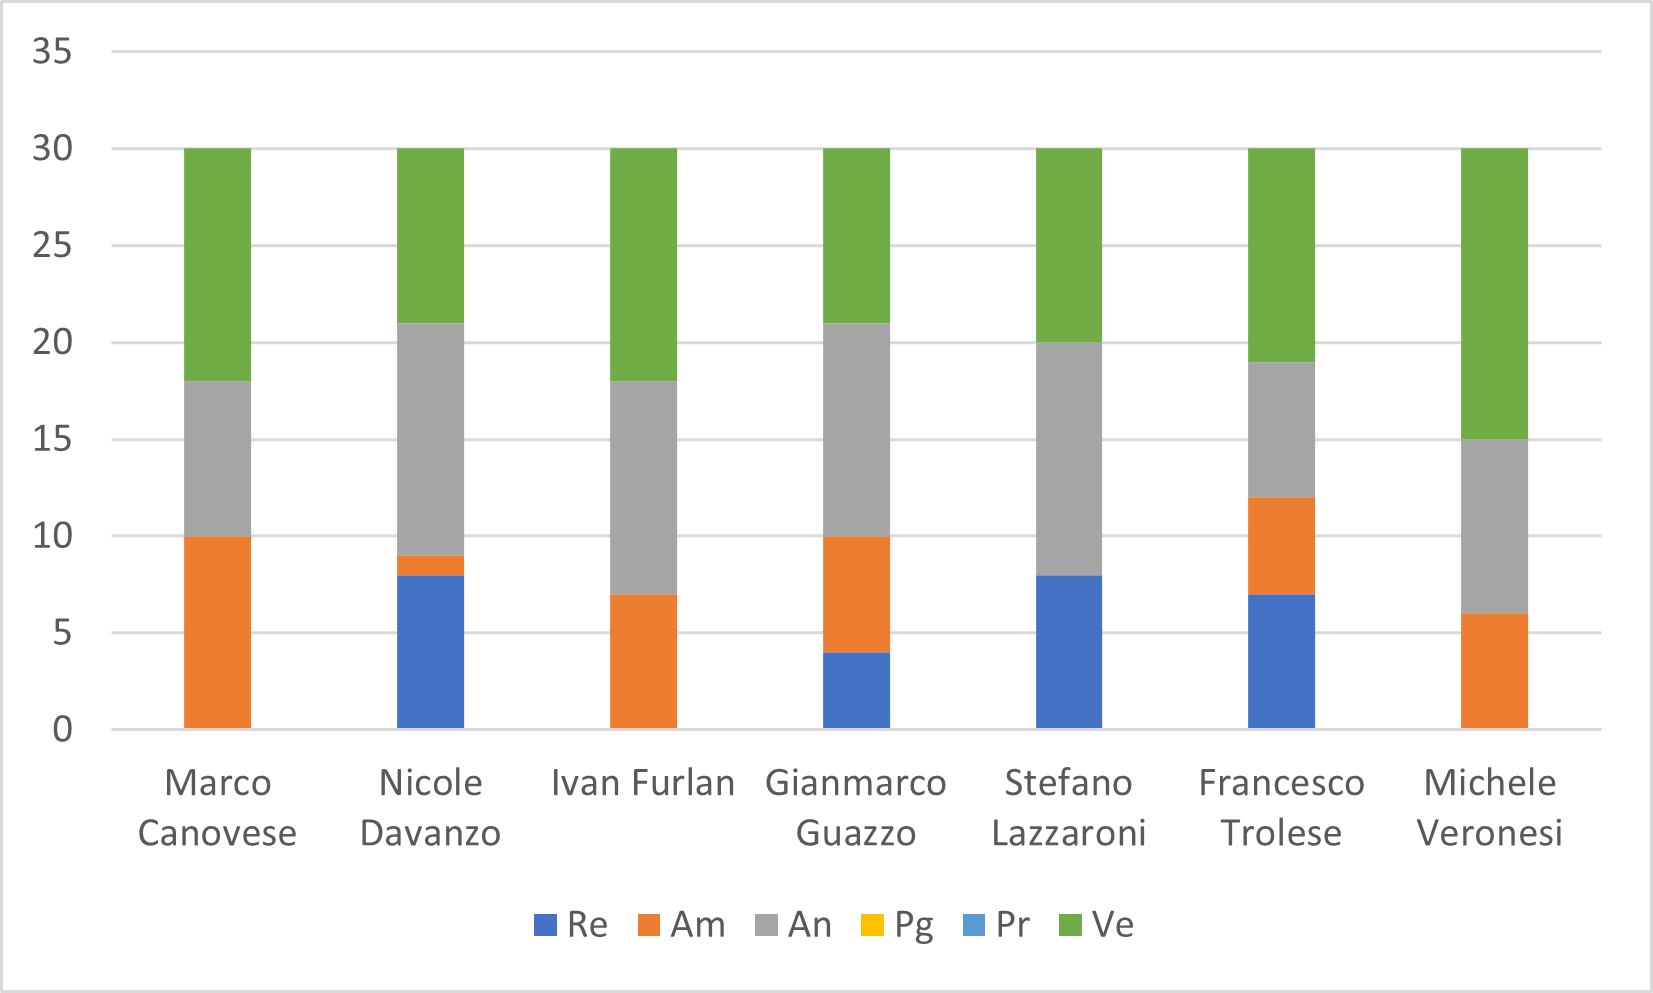
\includegraphics[width=0.8\linewidth]{res/images/preventivo/1-1.png}
	\caption{Diagramma ore/ruolo componenti nella fase di Analisi dei requisiti}
	\label{fig:diagramma suddivisione ruoli fase analisi dei requisiti}
\end{figure}

\paragraph{Prospetto economico}
In base al prospetto orario, quello economico sarà il seguente:

\rowcolors{1}{lightest-grayest}{blue!20}
\begin{longtable}{|l|c|c|c|c|c|c|c|}
	\hline
	\rowcolor{lighter-grayer}
	\textbf{Ruolo}  & \textbf{Ore} & \textbf{Costo in €} \\
	\hline
	\endfirsthead

	\hline
	Responsabile    & 27           & 810,00              \\
	\hline
	\hline
	Amministratore  & 35           & 700,00              \\
	\hline
	\hline
	Analista        & 70           & 1.750,00            \\
	\hline
	\hline
	Progettista     & -            & -                   \\
	\hline
	\hline
	Programmatore   & -            & -                   \\
	\hline
	\hline
	Verificatore    & 78           & 1.170,00            \\
	\hline
	\textbf{Totale} & 210          & 4.430,00            \\
	\hline
	\rowcolor{white}
	\caption{Tabella contenente il prospetto economico in riferimento al prospetto orario}
\end{longtable}
\pagebreak

La tabella può essere riassunta nel seguente areogramma:
\begin{figure}[H]
	\centering
	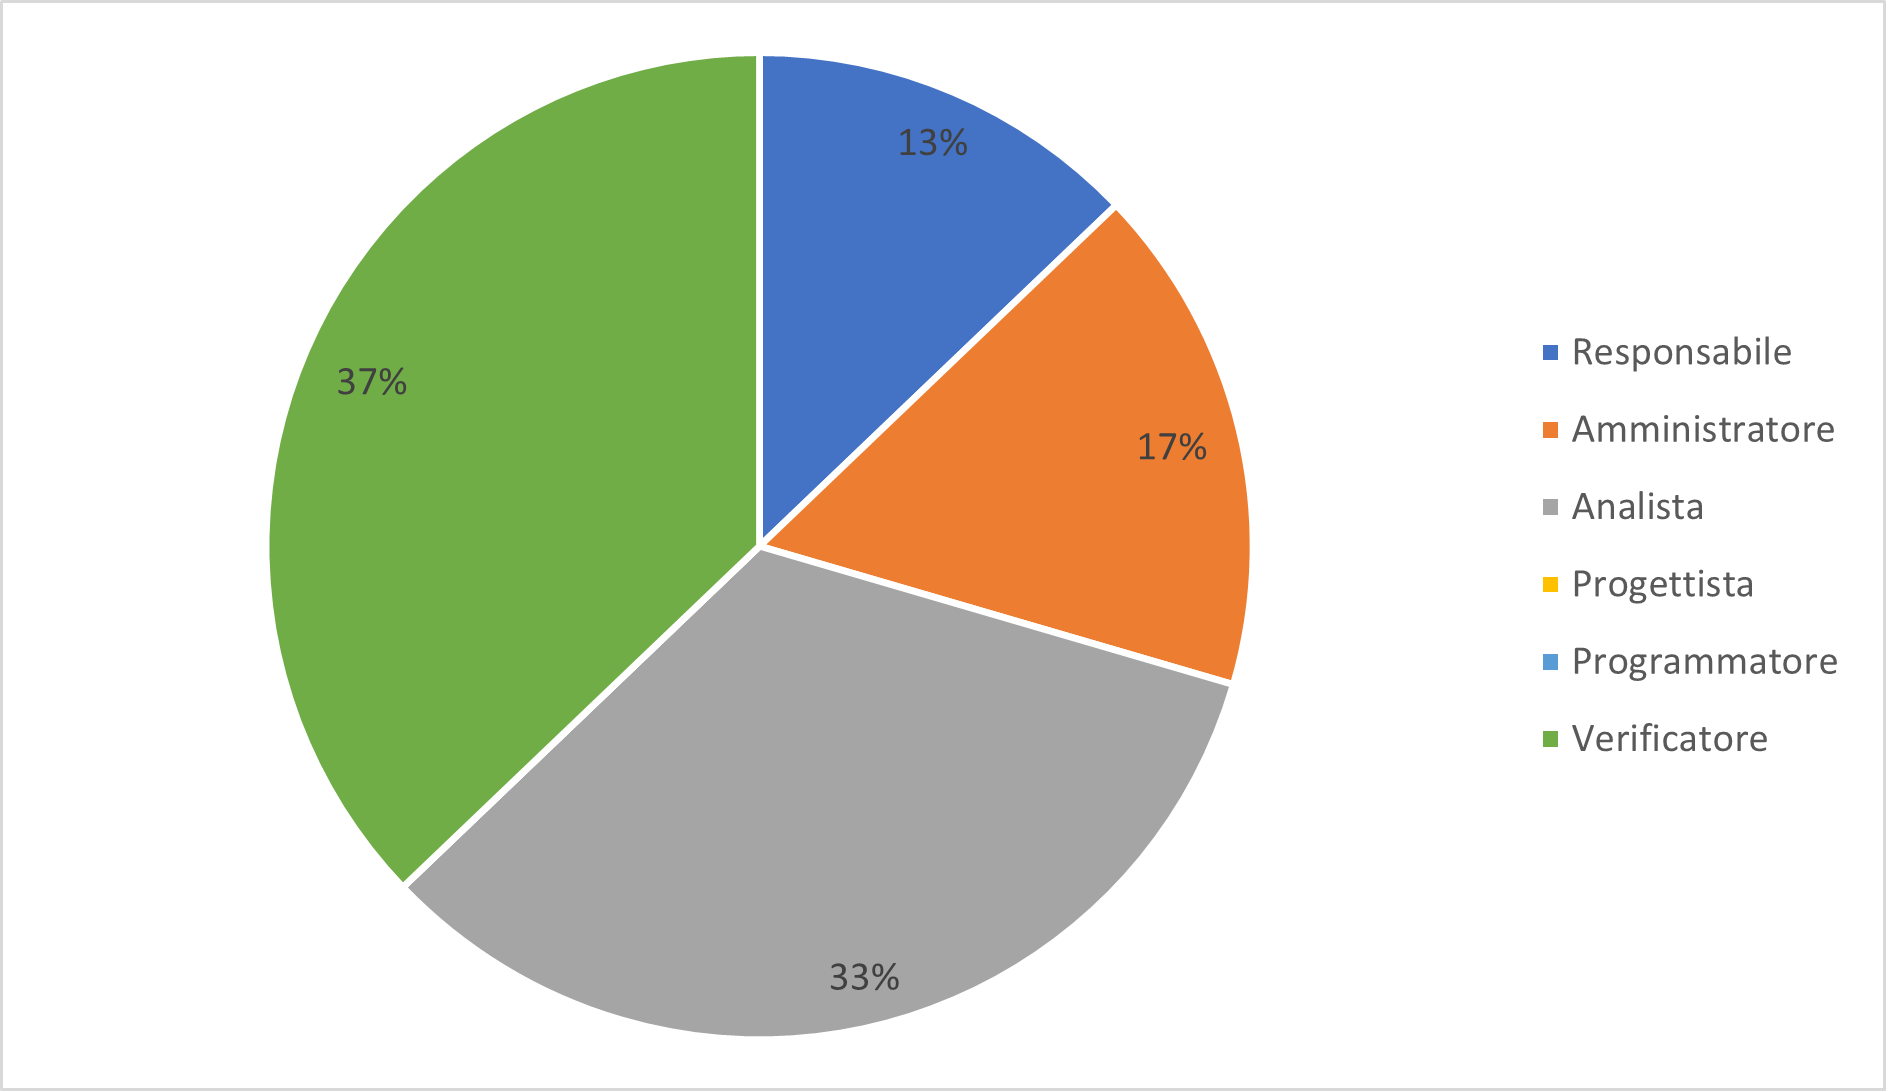
\includegraphics[width=0.8\linewidth]{res/images/preventivo/1-2.png}
	\caption{Diagramma percentuale ore/ruolo nella fase di Analisi dei requisiti}
	\label{fig:diagramma costi ruolo fase analisi dei requisiti}
\end{figure}

\subsection{Fase di consolidamento dei requisiti}
\subsubsection{Prospetto orario}
Durante la fase di consolidamento dei requisiti la distribuzione oraria sarà la seguente:

\rowcolors{1}{lightest-grayest}{blue!20}
\begin{longtable}{|l|c|c|c|c|c|c|c|}
	\hline
	\rowcolor{lighter-grayer}
	\textbf{Nome}     & \textbf{Re} & \textbf{Am} & \textbf{An} & \textbf{Pg} & \textbf{Pr} & \textbf{Ve} & \textbf{Totale} \\
	\hline
	\endfirsthead

	\hline
	Marco Canovese    & 2           & 0           & 3           & 0           & 0           & 0           & 5               \\
	\hline
	\hline
	Nicole Davanzo    & 0           & 0           & 3           & 0           & 0           & 2           & 5               \\
	\hline
	\hline
	Ivan Furlan       & 0           & 0           & 3           & 0           & 0           & 2           & 5               \\
	\hline
	\hline
	Gianmarco Guazzo  & 0           & 0           & 3           & 0           & 0           & 2           & 5               \\
	\hline
	\hline
	Stefano Lazzaroni & 0           & 5           & 0           & 0           & 0           & 0           & 5               \\
	\hline
	\hline
	Francesco Trolese & 0           & 0           & 1           & 0           & 0           & 4           & 5               \\
	\hline
	\hline
	Michele Veronesi  & 2           & 0           & 0           & 0           & 0           & 3           & 5               \\
	\hline
	\hline
	Totale            & 4           & 5           & 13          & 0           & 0           & 13          & 35              \\
	\hline
	\rowcolor{white}
	\caption{Tabella contenente il prospetto orario preventivato per la fase di consolidamento dei requisiti}
\end{longtable}


La tabella può essere riassunta nel seguente istogramma:

\begin{figure}[H]
	\centering
	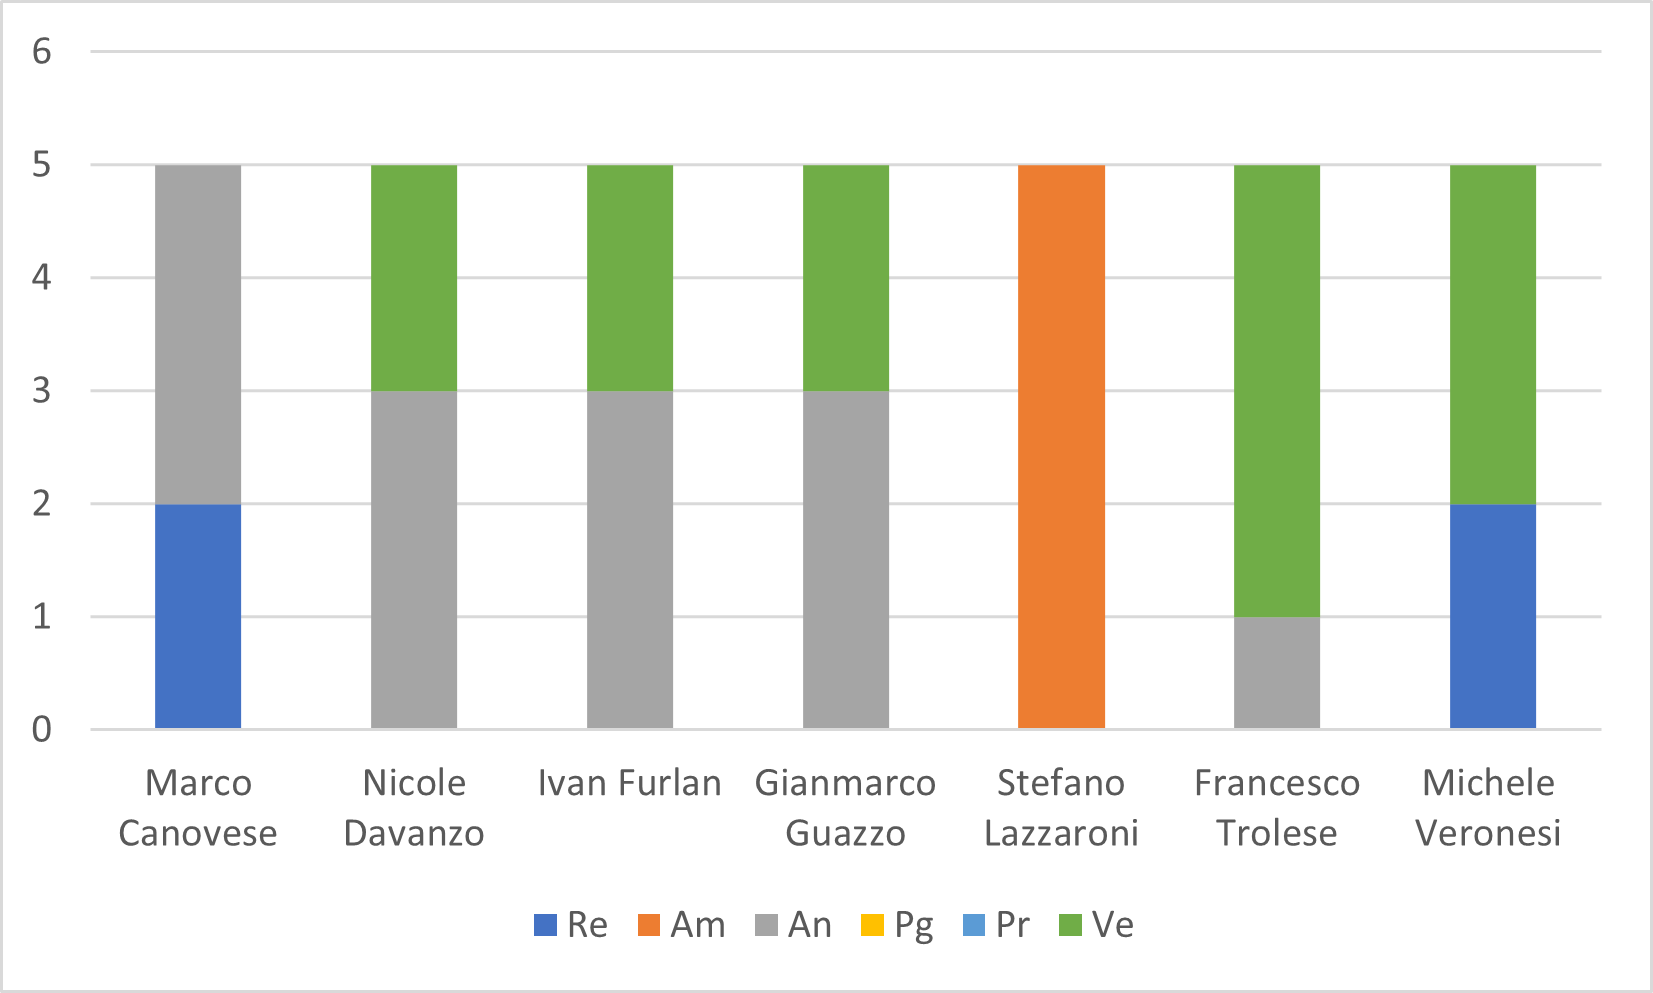
\includegraphics[width=0.8\linewidth]{res/images/preventivo/2-1.png}
	\caption{Diagramma ore/ruolo componenti nella fase di Consolidamento dei requisiti}
	\label{fig:diagramma suddivisione ruoli fase conslidamento dei requisiti}
\end{figure}

\subsubsection{Prospetto economico}
In base al prospetto orario, quello economico sarà il seguente:

\rowcolors{1}{lightest-grayest}{blue!20}
\begin{longtable}{|l|c|c|c|c|c|c|c|}
	\hline
	\rowcolor{lighter-grayer}
	\textbf{Ruolo}  & \textbf{Ore} & \textbf{Costo in €} \\
	\hline
	\endfirsthead

	\hline
	Responsabile    & 4            & 120,00              \\
	\hline
	\hline
	Amministratore  & 5            & 100,00              \\
	\hline
	\hline
	Analista        & 13           & 325,00              \\
	\hline
	\hline
	Progettista     & -            & -                   \\
	\hline
	\hline
	Programmatore   & -            & -                   \\
	\hline
	\hline
	Verificatore    & 13           & 195,00              \\
	\hline
	\hline
	\textbf{Totale} & 35           & 740,00              \\
	\hline
	\rowcolor{white}
	\caption{Tabella contenente il prospetto economico in riferimento al prospetto orario}
\end{longtable}
\pagebreak

La tabella può essere riassunta nel seguente areogramma:
\begin{figure}[H]
	\centering
	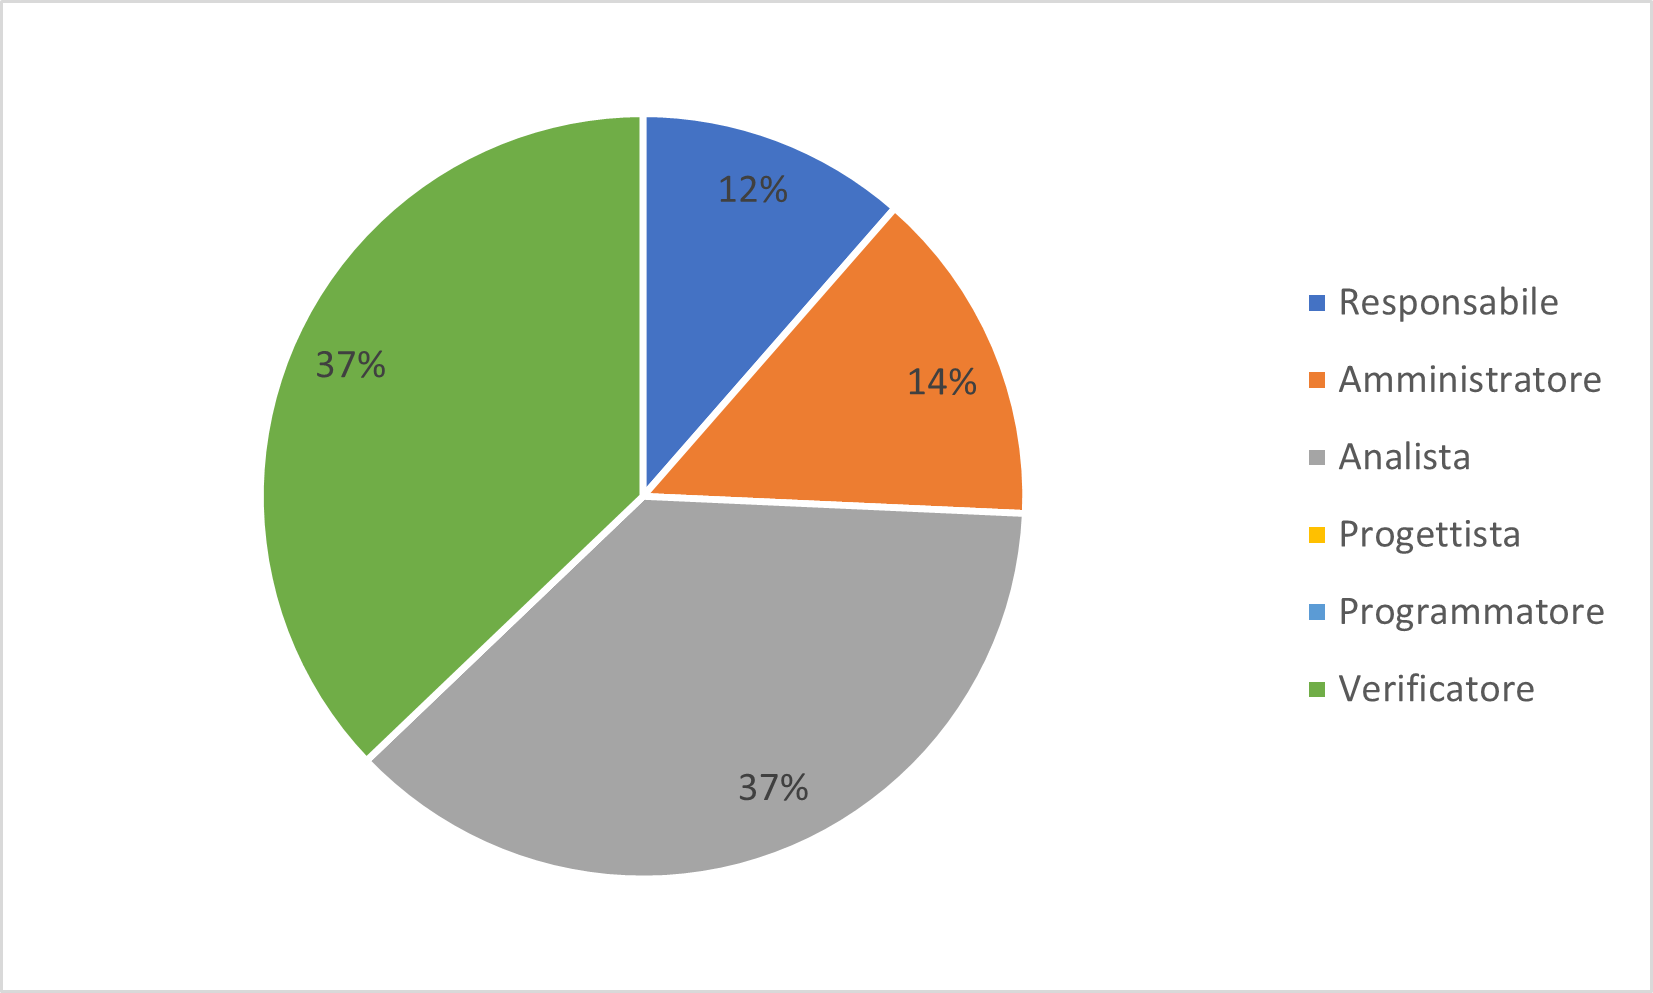
\includegraphics[width=0.8\linewidth]{res/images/preventivo/2-2.png}
	\caption{Diagramma percentuale ore/ruolo nella fase di Consolidamento dei requisiti}
	\label{fig:diagramma costi ruolo fase consolidamento dei requisiti}
\end{figure}

\subsection{Fase di progettazione della technology baseline}
\subsubsection{Prospetto orario}
Durante la fase di progettazione della technology baseline la distribuzione oraria sarà la seguente:

\rowcolors{1}{lightest-grayest}{blue!20}
\begin{longtable}{|l|c|c|c|c|c|c|c|}
	\hline
	\rowcolor{lighter-grayer}
	\textbf{Nome}     & \textbf{Re} & \textbf{Am} & \textbf{An} & \textbf{Pg} & \textbf{Pr} & \textbf{Ve} & \textbf{Totale} \\
	\hline
	\endfirsthead

	\hline
	Marco Canovese    & 0           & 5           & 3           & 0           & 0           & 4           & 12              \\
	\hline
	\hline
	Nicole Davanzo    & 0           & 5           & 0           & 6           & 0           & 1           & 12              \\
	\hline
	\hline
	Ivan Furlan       & 7           & 0           & 5           & 0           & 0           & 0           & 12              \\
	\hline
	\hline
	Gianmarco Guazzo  & 0           & 3           & 3           & 3           & 0           & 3           & 12              \\
	\hline
	\hline
	Stefano Lazzaroni & 0           & 0           & 3           & 9           & 0           & 0           & 12              \\
	\hline
	\hline
	Francesco Trolese & 0           & 2           & 6           & 0           & 0           & 4           & 12              \\
	\hline
	\hline
	Michele Veronesi  & 0           & 0           & 5           & 4           & 0           & 3           & 12              \\
	\hline
	\hline
	Totale            & 7           & 15          & 25          & 22          & 0           & 15          & 84              \\
	\hline
	\rowcolor{white}
	\caption{Tabella contenente il prospetto orario preventivato per la fase di progettazione della technology baseline.}
\end{longtable}


La tabella può essere riassunta nel seguente istogramma:

\begin{figure}[H]
	\centering
	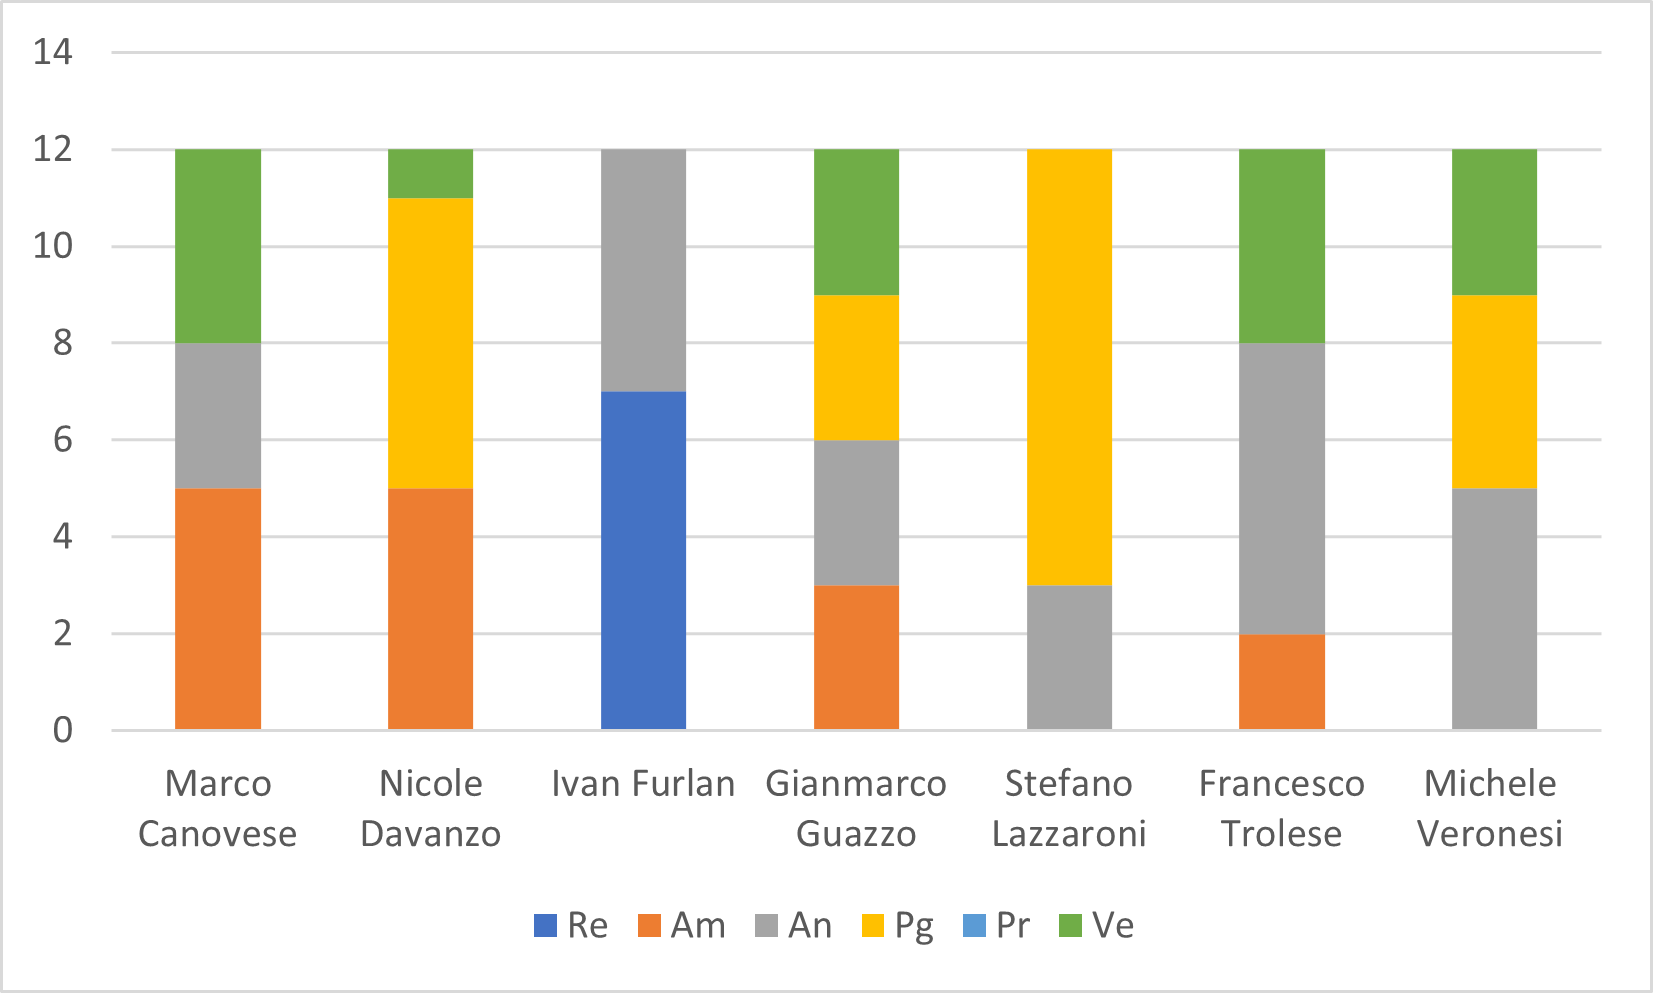
\includegraphics[width=0.8\linewidth]{res/images/preventivo/3-1.png}
	\caption{Diagramma ore/ruolo componenti nella fase di Progettazione della technology baseline }
	\label{fig:diagramma suddivisione ruoli fase progettazione della technology baseline}
\end{figure}

\subsubsection{Prospetto economico}
In base al prospetto orario, quello economico sarà il seguente:

\rowcolors{1}{lightest-grayest}{blue!20}
\begin{longtable}{|l|c|c|c|c|c|c|c|}
	\hline
	\rowcolor{lighter-grayer}
	\textbf{Ruolo}  & \textbf{Ore} & \textbf{Costo in €} \\
	\hline
	\endfirsthead

	\hline
	Responsabile    & 7            & 210,00              \\
	\hline
	\hline
	Amministratore  & 15           & 300,00              \\
	\hline
	\hline
	Analista        & 25           & 625,00              \\
	\hline
	\hline
	Progettista     & 22           & 484,00              \\
	\hline
	\hline
	Programmatore   & -            & -                   \\
	\hline
	\hline
	Verificatore    & 15           & 225,00              \\
	\hline
	\hline
	\textbf{Totale} & 84           & 1.844,00            \\
	\hline
	\rowcolor{white}
	\caption{Tabella contenente il prospetto economico in riferimento al prospetto orario}
\end{longtable}
\pagebreak

La tabella può essere riassunta nel seguente areogramma:
\begin{figure}[H]
	\centering
	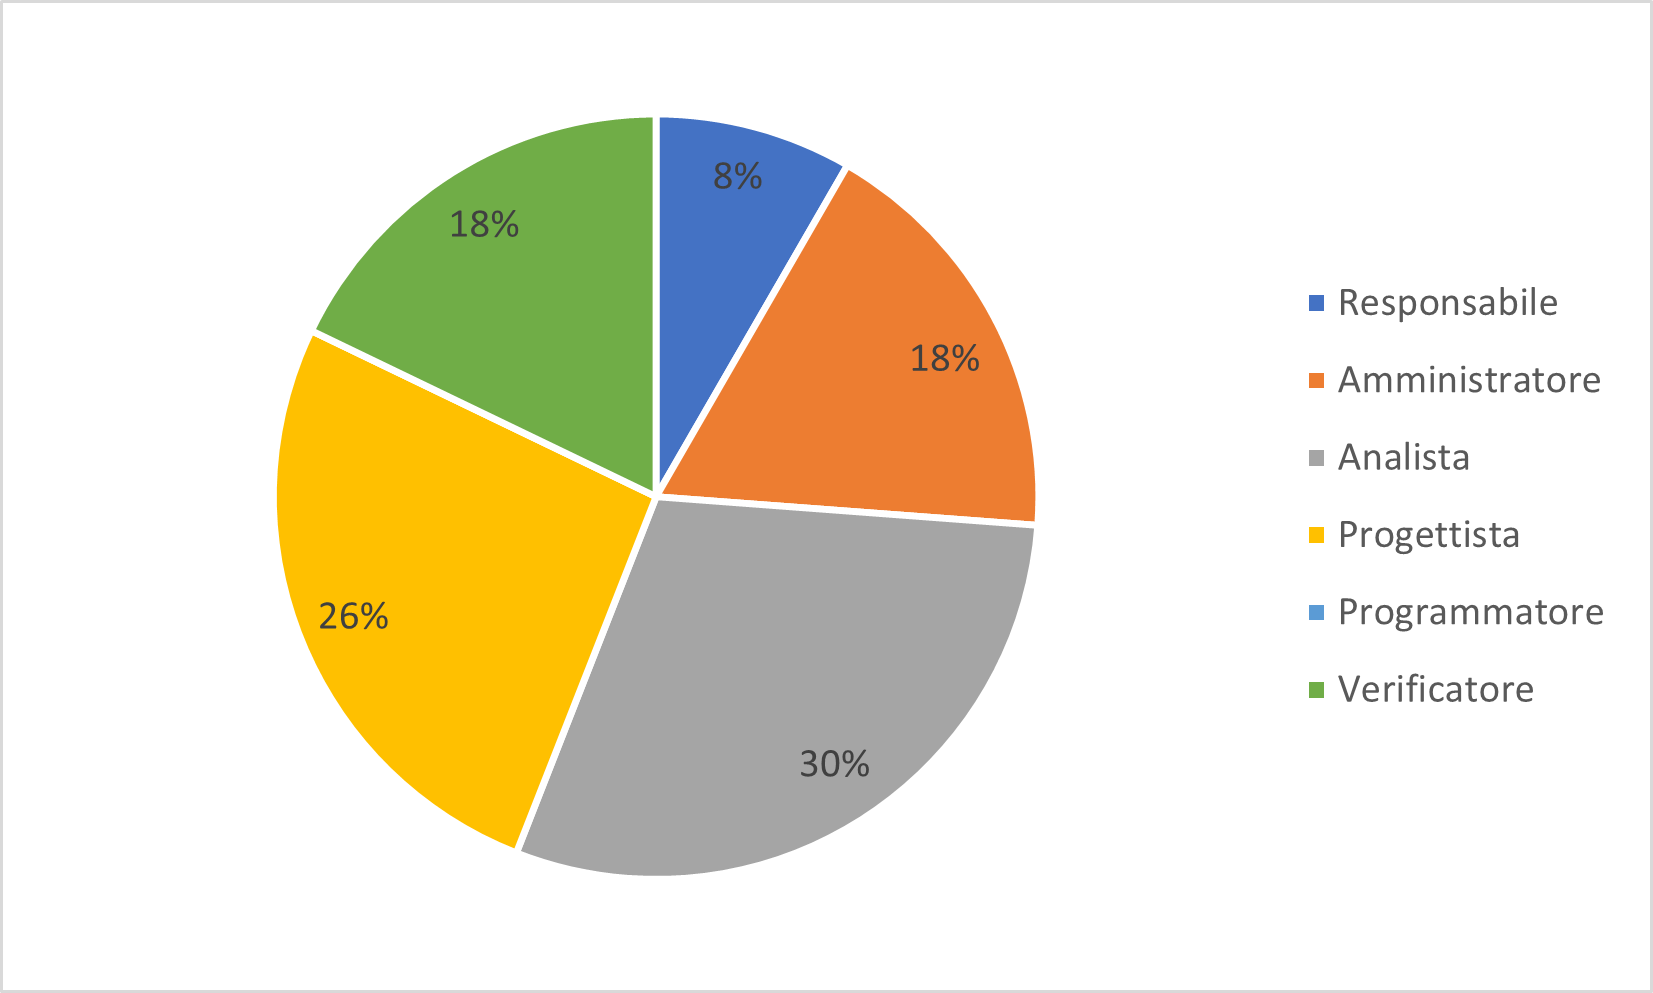
\includegraphics[width=0.8\linewidth]{res/images/preventivo/3-2.png}
	\caption{Diagramma percentuale ore/ruolo nella fase di Progettazione della technology baseline }
	\label{fig:diagramma costi ruolo fase progettazione della technology baseline }
\end{figure}

\subsection{Fase di progettazione e codifica del Proof of Concept}
La fase è composta da tre incrementi caratterizzati dalla distribuzione oraria descritta di seguito.

\subsubsection{I incremento}
\paragraph{Prospetto orario}
Durante il I incremento la distribuzione oraria sarà la seguente:

\rowcolors{1}{lightest-grayest}{blue!20}
\begin{longtable}{|l|c|c|c|c|c|c|c|}
	\hline
	\rowcolor{lighter-grayer}
	\textbf{Nome}     & \textbf{Re} & \textbf{Am} & \textbf{An} & \textbf{Pg} & \textbf{Pr} & \textbf{Ve} & \textbf{Totale} \\
	\hline
	\endfirsthead

	\hline
	Marco Canovese    & 2           & 0           & 0           & 4           & 0           & 2           & 8               \\
	\hline
	\hline
	Nicole Davanzo    & 0           & 3           & 0           & 0           & 0           & 5           & 8               \\
	\hline
	\hline
	Ivan Furlan       & 2           & 2           & 0           & 0           & 2           & 2           & 8               \\
	\hline
	\hline
	Gianmarco Guazzo  & 0           & 3           & 0           & 3           & 2           & 0           & 8               \\
	\hline
	\hline
	Stefano Lazzaroni & 0           & 0           & 0           & 4           & 3           & 1           & 8               \\
	\hline
	\hline
	Francesco Trolese & 0           & 2           & 0           & 4           & 0           & 2           & 8               \\
	\hline
	\hline
	Michele Veronesi  & 3           & 0           & 0           & 2           & 3           & 0           & 8               \\
	\hline
	\hline
	Totale            & 7           & 10          & 0          & 17           & 10           & 12           & 56              \\
	\hline
	\rowcolor{white}
	\caption{Tabella contenente il prospetto orario preventivato per il I incremento}
\end{longtable}


La tabella può essere riassunta nel seguente istogramma:

\begin{figure}[H]
	\centering
	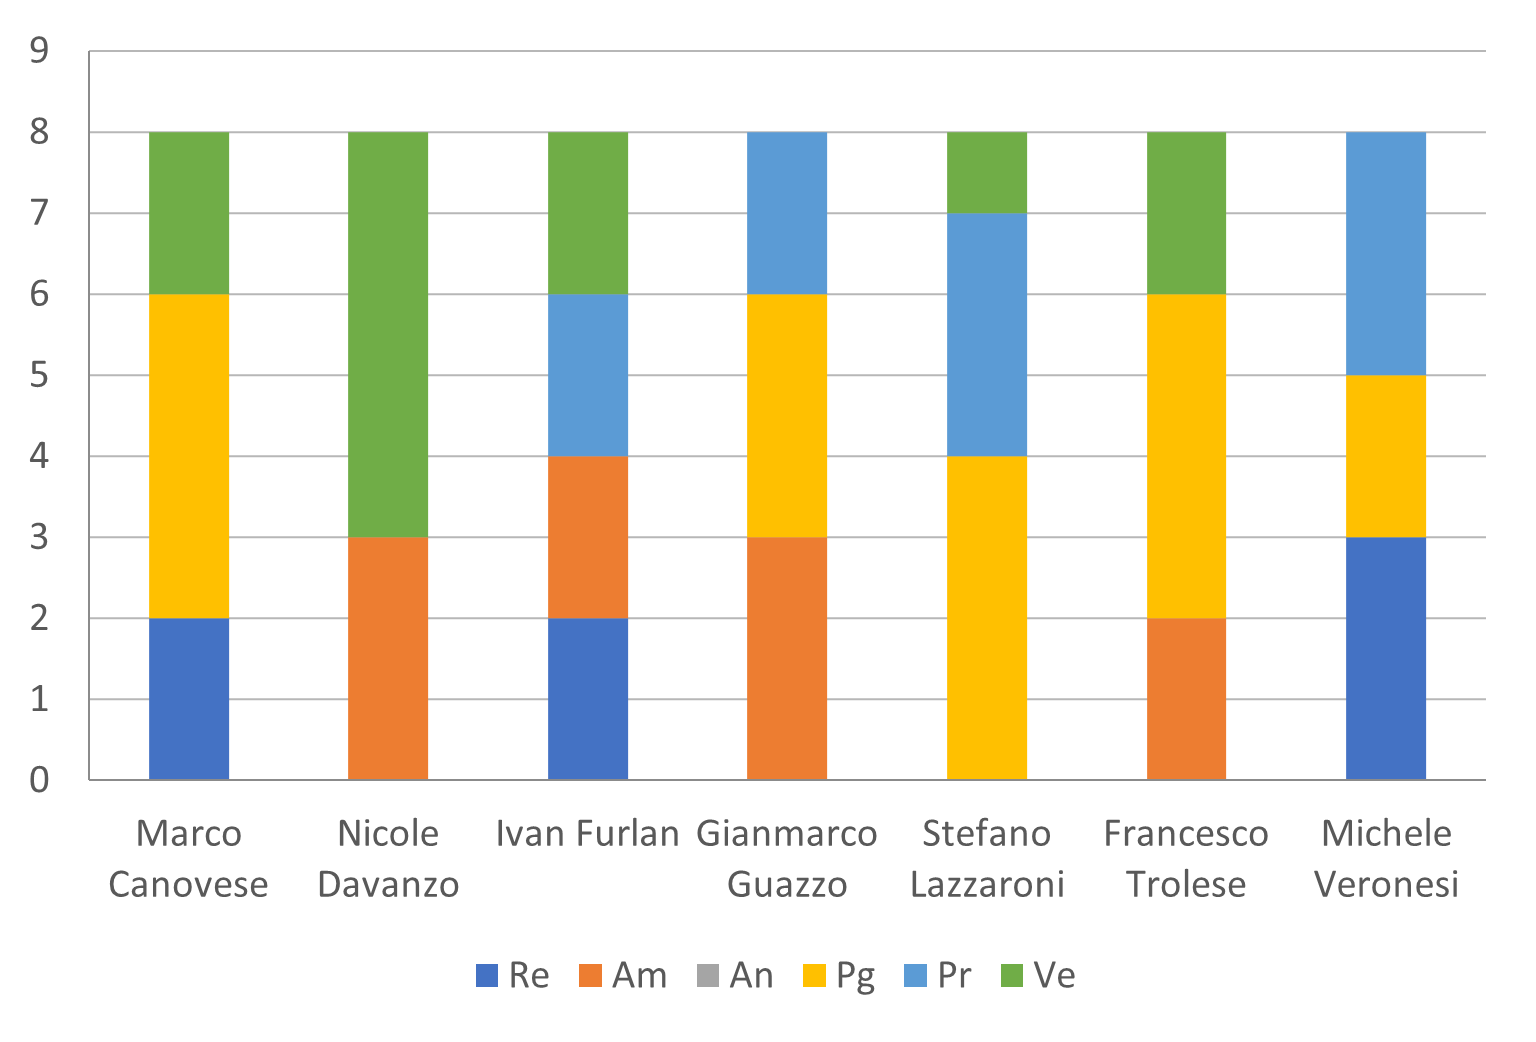
\includegraphics[width=0.8\linewidth]{res/images/preventivo/dettaglio_poc/1-1.png}
	\caption{Diagramma ore/ruolo componenti nel I incremento}
	\label{fig:diagramma suddivisione ruoli I incremento}
\end{figure}

\paragraph{Prospetto economico}
In base al prospetto orario, quello economico sarà il seguente:

\rowcolors{1}{lightest-grayest}{blue!20}
\begin{longtable}{|l|c|c|c|c|c|c|c|}
	\hline
	\rowcolor{lighter-grayer}
	\textbf{Ruolo}  & \textbf{Ore} & \textbf{Costo in €} \\
	\hline
	\endfirsthead

	\hline
	Responsabile    & 7            & 210,00              \\
	\hline
	\hline
	Amministratore  & 10           & 200,00              \\
	\hline
	\hline
	Analista        & 0           & 00,00              \\
	\hline
	\hline
	Progettista     & 17            & 374,00                   \\
	\hline
	\hline
	Programmatore   & 10            & 150,00                   \\
	\hline
	\hline
	Verificatore    & 12            & 180,00                   \\
	\hline
	\textbf{Totale} & 56           & 1.114,00            \\
	\hline
	\rowcolor{white}
	\caption{Tabella contenente il prospetto economico in riferimento al prospetto orario}
\end{longtable}
\pagebreak

La tabella può essere riassunta nel seguente areogramma:
\begin{figure}[H]
	\centering
	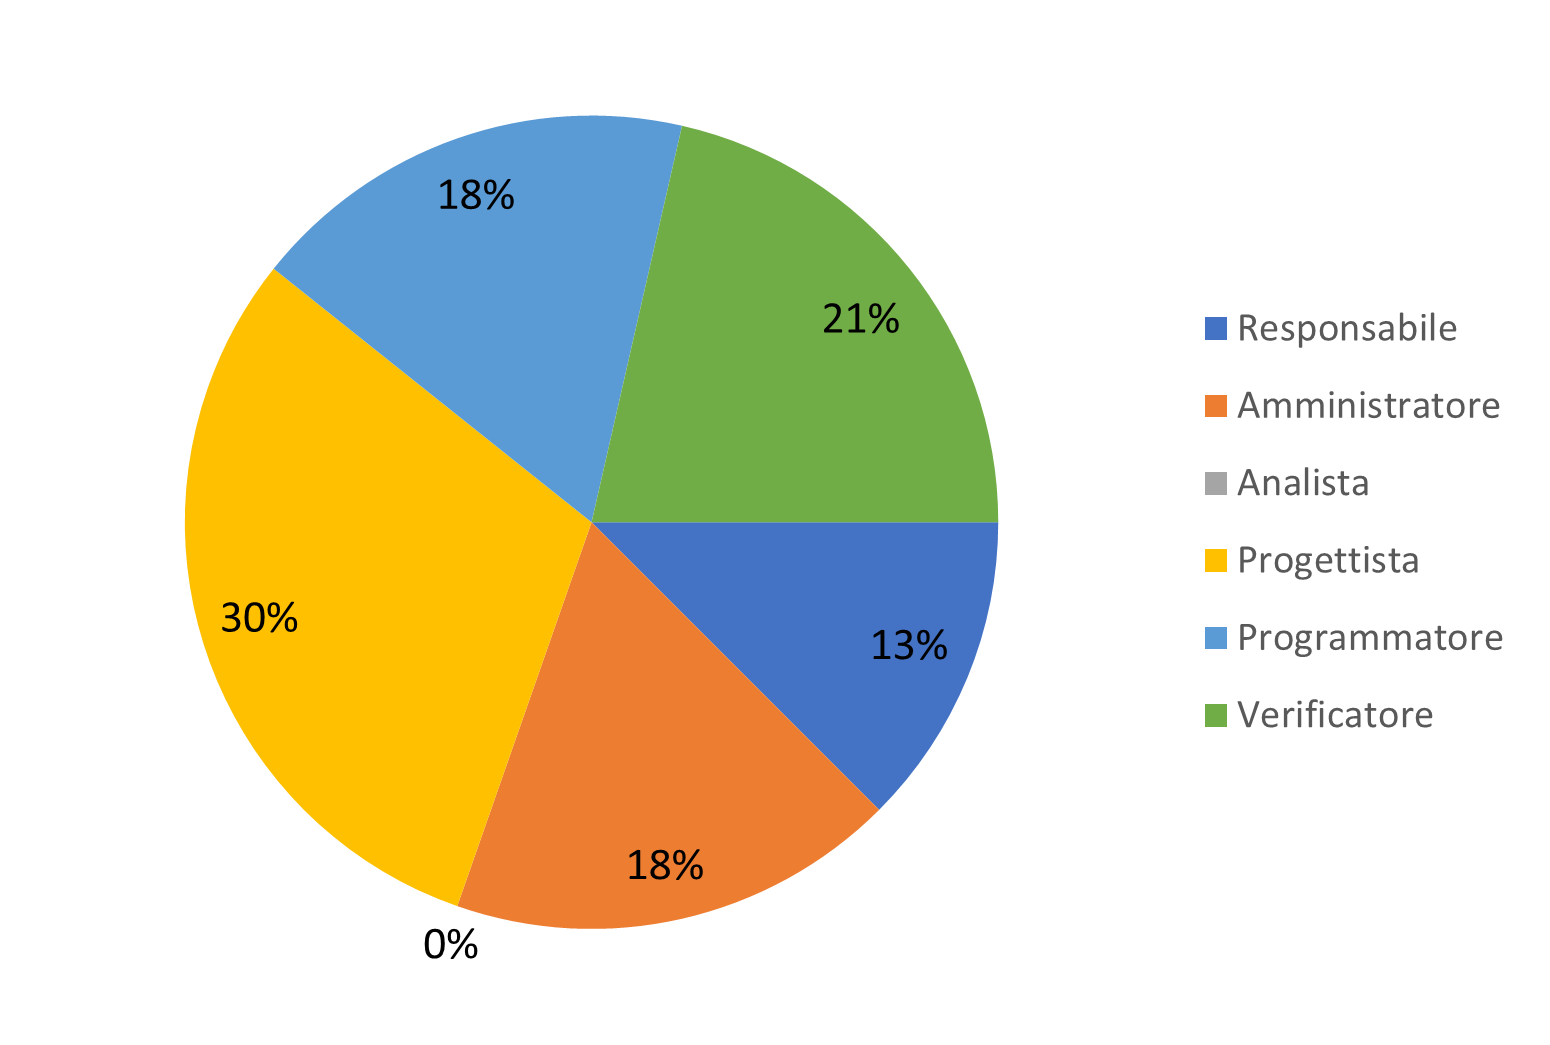
\includegraphics[width=0.8\linewidth]{res/images/preventivo/dettaglio_poc/1-2.png}
	\caption{Diagramma percentuale ore/ruolo nel I incremento}
	\label{fig:diagramma costi ruolo  I incremento}
\end{figure}

\subsubsection{II incremento}
\paragraph{Prospetto orario}
Durante il II incremento la distribuzione oraria sarà la seguente:

\rowcolors{1}{lightest-grayest}{blue!20}
\begin{longtable}{|l|c|c|c|c|c|c|c|}
	\hline
	\rowcolor{lighter-grayer}
	\textbf{Nome}     & \textbf{Re} & \textbf{Am} & \textbf{An} & \textbf{Pg} & \textbf{Pr} & \textbf{Ve} & \textbf{Totale} \\
	\hline
	\endfirsthead

	\hline
	Marco Canovese    & 2           & 0           & 0           & 2           & 3           & 2           & 9               \\
	\hline
	\hline
	Nicole Davanzo    & 0           & 1           & 0           & 2           & 4           & 2           & 9               \\
	\hline
	\hline
	Ivan Furlan       & 1           & 1           & 0           & 0           & 4           & 3           & 9               \\
	\hline
	\hline
	Gianmarco Guazzo  & 1           & 2           & 0           & 2           & 2           & 2           & 9               \\
	\hline
	\hline
	Stefano Lazzaroni & 0           & 2           & 0           & 2           & 3           & 2           & 9               \\
	\hline
	\hline
	Francesco Trolese & 0           & 0           & 3           & 2           & 2           & 2           & 9               \\
	\hline
	\hline
	Michele Veronesi  & 2           & 0           & 0           & 0           & 3           & 4           & 9               \\
	\hline
	\hline
	Totale            & 6           & 6          & 3          & 10           & 21           & 17          & 63              \\
	\hline
	\rowcolor{white}
	\caption{Tabella contenente il prospetto orario preventivato per il II incremento}
\end{longtable}


La tabella può essere riassunta nel seguente istogramma:

\begin{figure}[H]
	\centering
	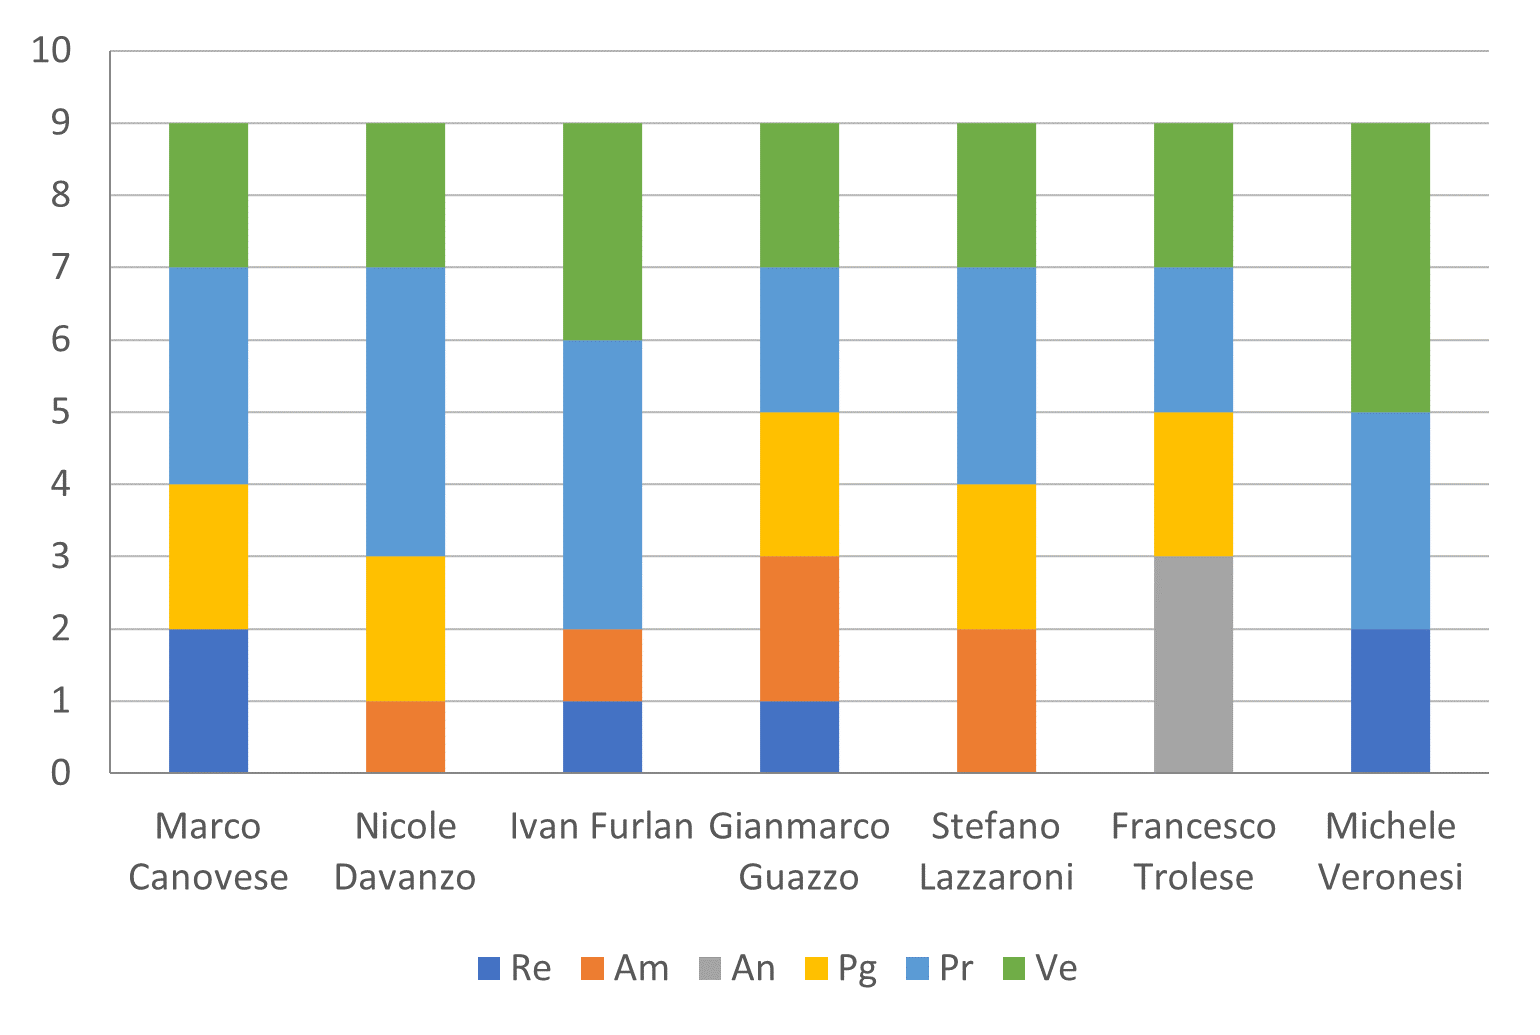
\includegraphics[width=0.8\linewidth]{res/images/preventivo/dettaglio_poc/2-1.png}
	\caption{Diagramma ore/ruolo componenti nel II incremento}
	\label{fig:diagramma suddivisione ruoli II incremento}
\end{figure}

\paragraph{Prospetto economico}
In base al prospetto orario, quello economico sarà il seguente:

\rowcolors{1}{lightest-grayest}{blue!20}
\begin{longtable}{|l|c|c|c|c|c|c|c|}
	\hline
	\rowcolor{lighter-grayer}
	\textbf{Ruolo}  & \textbf{Ore} & \textbf{Costo in €} \\
	\hline
	\endfirsthead

	\hline
	Responsabile    & 6            & 180,00              \\
	\hline
	\hline
	Amministratore  & 6           & 120,00              \\
	\hline
	\hline
	Analista        & 3           & 75,00              \\
	\hline
	\hline
	Progettista     & 10            & 220,00                   \\
	\hline
	\hline
	Programmatore   & 21            & 315,00                   \\
	\hline
	\hline
	Verificatore    & 17           & 255,00              \\
	\hline
	\hline
	\textbf{Totale} & 63           & 1.165,00            \\
	\hline
	\rowcolor{white}
	\caption{Tabella contenente il prospetto economico in riferimento al prospetto orario}
\end{longtable}
\pagebreak

La tabella può essere riassunta nel seguente areogramma:
\begin{figure}[H]
	\centering
	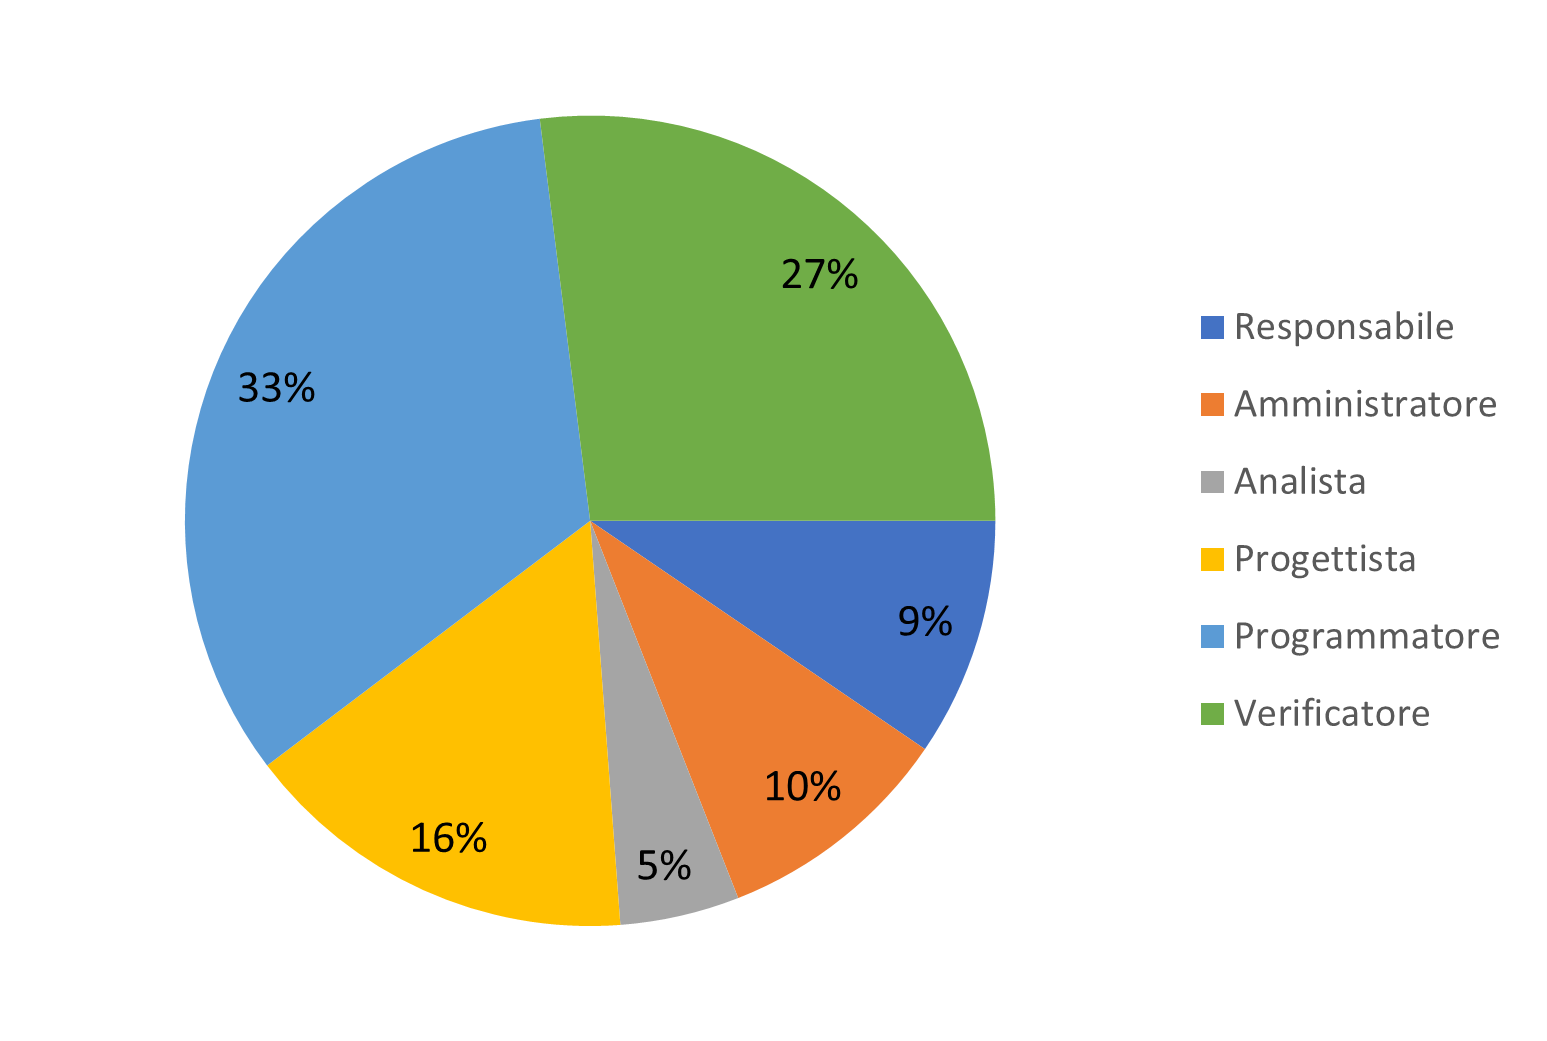
\includegraphics[width=0.8\linewidth]{res/images/preventivo/dettaglio_poc/2-2.png}
	\caption{Diagramma percentuale ore/ruolo nel II incremento}
	\label{fig:diagramma costi ruolo II incremento}
\end{figure}

\subsubsection{III incremento}
\paragraph{Prospetto orario}
Durante il III incremento la distribuzione oraria sarà la seguente:

\rowcolors{1}{lightest-grayest}{blue!20}
\begin{longtable}{|l|c|c|c|c|c|c|c|}
	\hline
	\rowcolor{lighter-grayer}
	\textbf{Nome}     & \textbf{Re} & \textbf{Am} & \textbf{An} & \textbf{Pg} & \textbf{Pr} & \textbf{Ve} & \textbf{Totale} \\
	\hline
	\endfirsthead

	\hline
	Marco Canovese    & 0           & 0           & 0           & 1           & 6           & 0           & 7               \\
	\hline
	\hline
	Nicole Davanzo    & 0           & 1           & 0           & 6           & 0           & 0           & 7               \\
	\hline
	\hline
	Ivan Furlan       & 1           & 0           & 0           & 0           & 2           & 4           & 7               \\
	\hline
	\hline
	Gianmarco Guazzo  & 2           & 0           & 0           & 3           & 1           & 1           & 7               \\
	\hline
	\hline
	Stefano Lazzaroni & 0           & 0           & 0           & 3           & 0           & 4           & 7               \\
	\hline
	\hline
	Francesco Trolese & 0           & 0           & 0           & 0           & 7           & 0           & 7               \\
	\hline
	\hline
	Michele Veronesi  & 0           & 0           & 5           & 2           & 0           & 0           & 7               \\
	\hline
	\hline
	Totale            & 3           & 1           & 5          & 15           & 16           & 9          & 49              \\
	\hline
	\rowcolor{white}
	\caption{Tabella contenente il prospetto orario preventivato per il III incremento}
\end{longtable}


La tabella può essere riassunta nel seguente istogramma:

\begin{figure}[H]
	\centering
	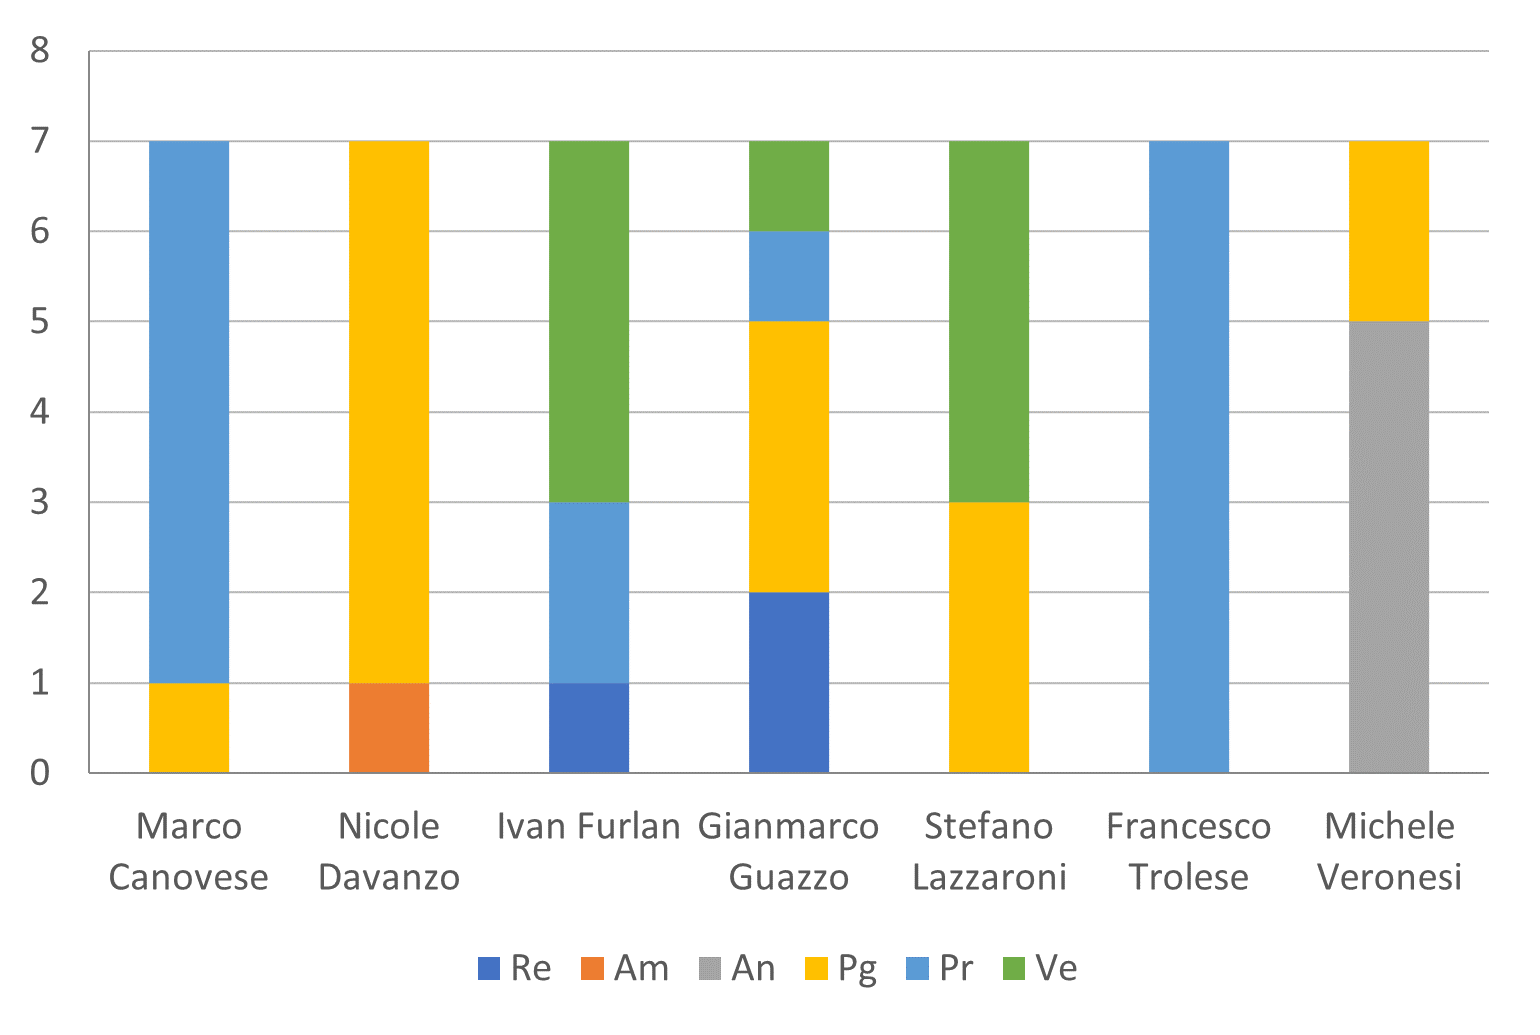
\includegraphics[width=0.8\linewidth]{res/images/preventivo/dettaglio_poc/3-1.png}
	\caption{Diagramma ore/ruolo componenti nel III incremento}
	\label{fig:diagramma suddivisione ruoli III incremento}
\end{figure}

\paragraph{Prospetto economico}
In base al prospetto orario, quello economico sarà il seguente:

\rowcolors{1}{lightest-grayest}{blue!20}
\begin{longtable}{|l|c|c|c|c|c|c|c|}
	\hline
	\rowcolor{lighter-grayer}
	\textbf{Ruolo}  & \textbf{Ore} & \textbf{Costo in €} \\
	\hline
	\endfirsthead

	\hline
	Responsabile    & 3            & 90,00              \\
	\hline
	\hline
	Amministratore  & 1            & 20,00               \\
	\hline
	\hline
	Analista        & 5           & 125,00              \\
	\hline
	\hline
	Progettista     & 15            & 330,00                   \\
	\hline
	\hline
	Programmatore   & 16            & 240,00                   \\
	\hline
	\hline
	Verificatore    & 9           & 135,00              \\
	\hline
	\textbf{Totale} & 49           & 940,00            \\
	\hline
	\rowcolor{white}
	\caption{Tabella contenente il prospetto economico in riferimento al prospetto orario}
\end{longtable}
\pagebreak

La tabella può essere riassunta nel seguente areogramma:
\begin{figure}[H]
	\centering
	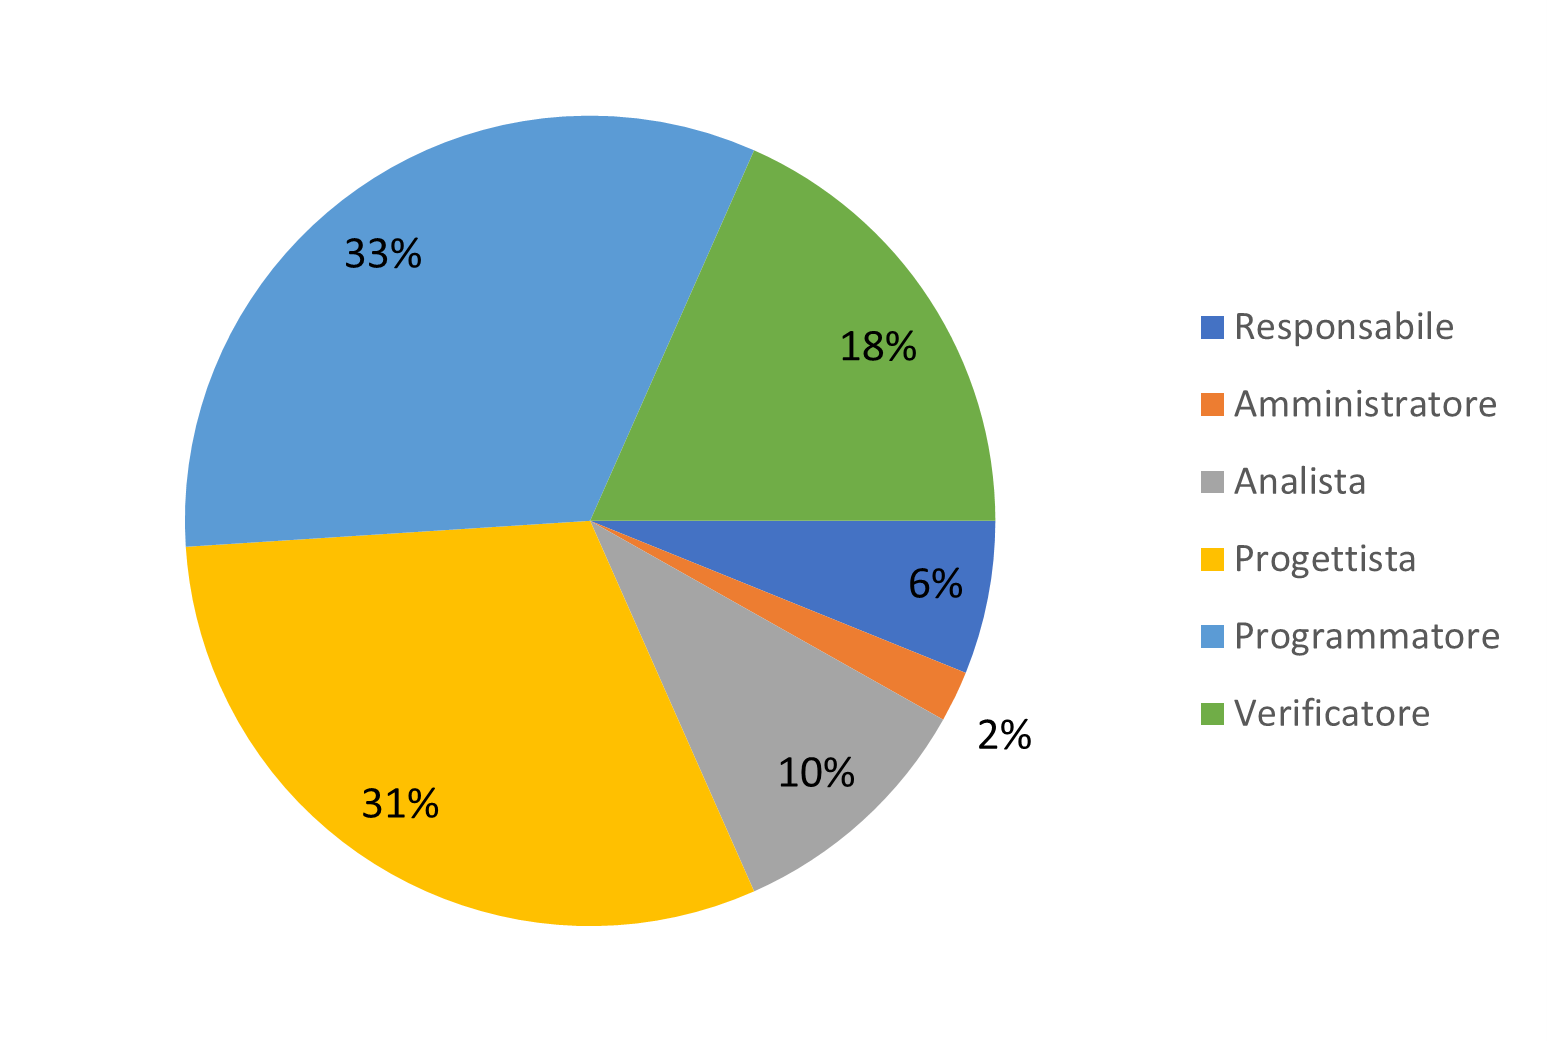
\includegraphics[width=0.8\linewidth]{res/images/preventivo/dettaglio_poc/3-2.png}
	\caption{Diagramma percentuale ore/ruolo nel III incremento}
	\label{fig:diagramma costi ruolo III incremento}
\end{figure}

\subsubsection{Fase complessiva}
\paragraph{Prospetto orario}
Durante la fase di progettazione della proof of concept la distribuzione oraria sarà la seguente:

\rowcolors{1}{lightest-grayest}{blue!20}
\begin{longtable}{|l|c|c|c|c|c|c|c|}
	\hline
	\rowcolor{lighter-grayer}
	\textbf{Nome}     & \textbf{Re} & \textbf{Am} & \textbf{An} & \textbf{Pg} & \textbf{Pr} & \textbf{Ve} & \textbf{Totale} \\
	\hline
	\endfirsthead

	\hline
	Marco Canovese    & 4           & 0           & 0           & 7           & 9           & 4           & 24              \\
	\hline
	\hline
	Nicole Davanzo    & 0           & 5           & 0           & 8           & 4           & 7           & 24              \\
	\hline
	\hline
	Ivan Furlan       & 4           & 3           & 0           & 0           & 8           & 9           & 24              \\
	\hline
	\hline
	Gianmarco Guazzo  & 3           & 5           & 0           & 8           & 5           & 3           & 24              \\
	\hline
	\hline
	Stefano Lazzaroni & 0           & 2           & 0           & 9           & 6           & 7           & 24              \\
	\hline
	\hline
	Francesco Trolese & 0           & 2           & 3           & 6           & 9           & 4           & 24              \\
	\hline
	\hline
	Michele Veronesi  & 5           & 0           & 5           & 4           & 6           & 4           & 24              \\
	\hline
	\hline
	Totale            & 16          & 17          & 8           & 42          & 47          & 38          & 168             \\
	\hline
	\rowcolor{white}
	\caption{Tabella contenente il prospetto orario preventivato per la fase di progettazione della proof of concept.}
\end{longtable}


La tabella può essere riassunta nel seguente istogramma:

\begin{figure}[H]
	\centering
	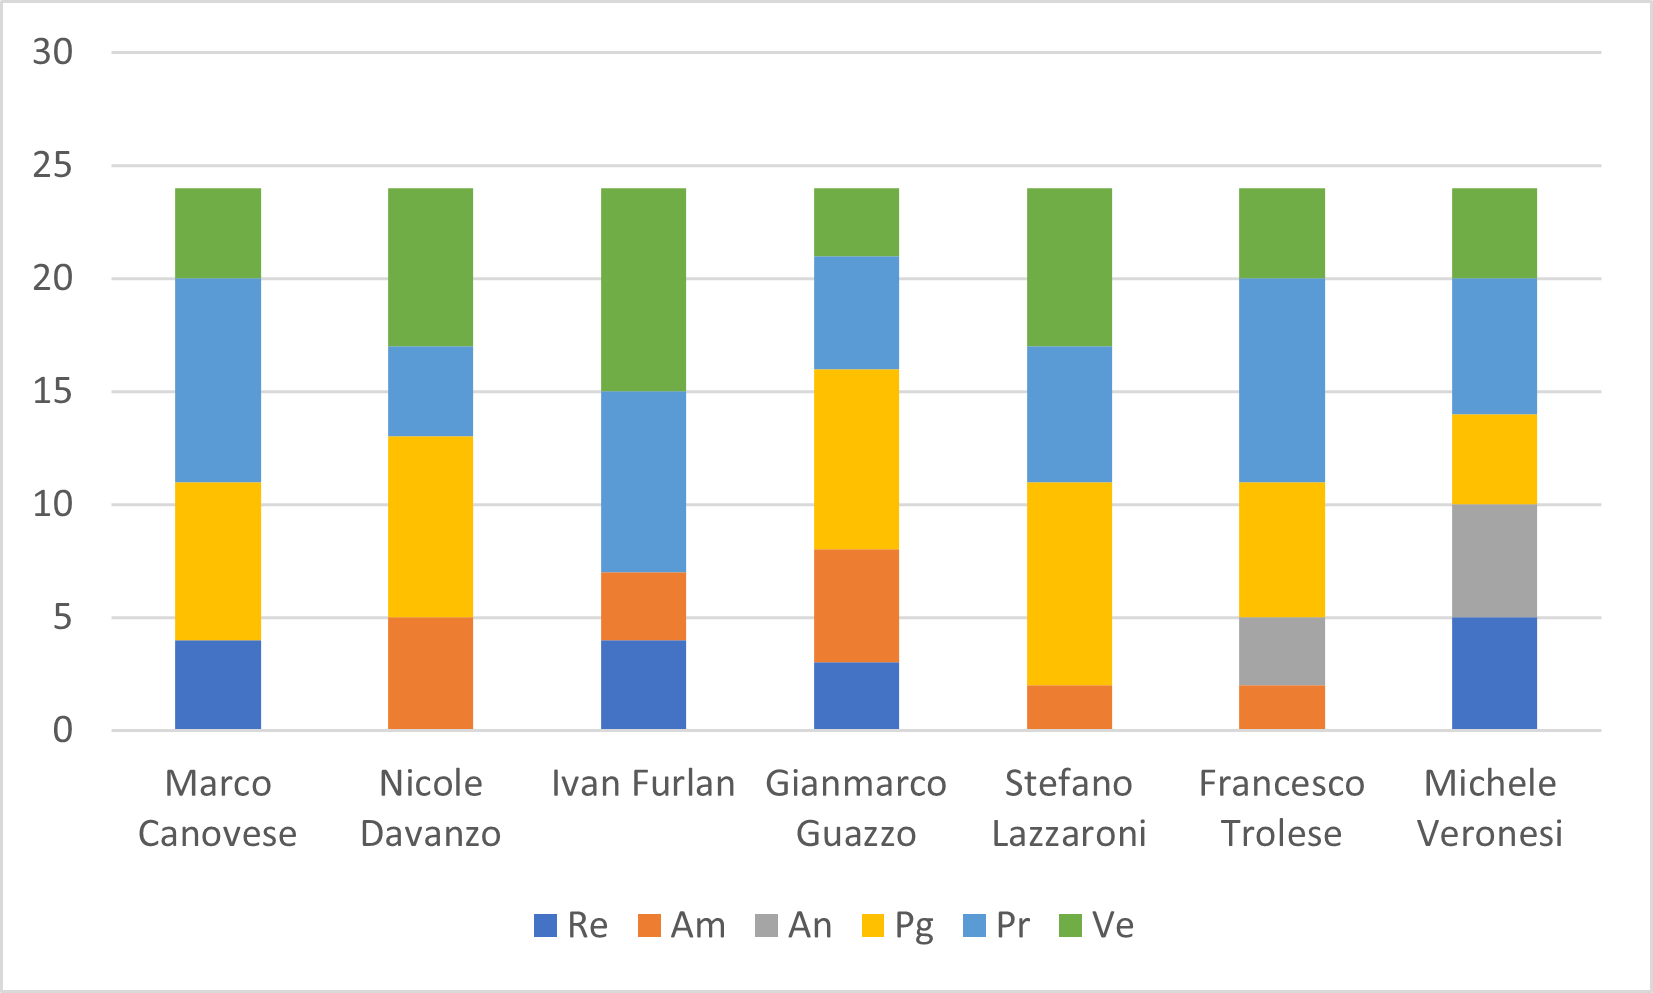
\includegraphics[width=0.8\linewidth]{res/images/preventivo/4-1.png}
	\caption{Diagramma ore/ruolo componenti nella fase di Progettazione della proof of concept}
	\label{fig:diagramma suddivisione ruoli fase progettazione della proof of concept}
\end{figure}

\paragraph{Prospetto economico}
In base al prospetto orario, quello economico sarà il seguente:

\rowcolors{1}{lightest-grayest}{blue!20}
\begin{longtable}{|l|c|c|c|c|c|c|c|}
	\hline
	\rowcolor{lighter-grayer}
	\textbf{Ruolo}  & \textbf{Ore} & \textbf{Costo in €} \\
	\hline
	\endfirsthead

	\hline
	Responsabile    & 16           & 480,00              \\
	\hline
	\hline
	Amministratore  & 17           & 340,00              \\
	\hline
	\hline
	Analista        & 8            & 200,00              \\
	\hline
	\hline
	Progettista     & 42           & 924,00              \\
	\hline
	\hline
	Programmatore   & 47           & 705,00              \\
	\hline
	\hline
	Verificatore    & 38           & 570,00              \\
	\hline
	\hline
	\textbf{Totale} & 168          & 3.219,00            \\
	\hline
	\rowcolor{white}
	\caption{Tabella contenente il prospetto economico in riferimento al prospetto orario}
\end{longtable}
\pagebreak

La tabella può essere riassunta nel seguente areogramma:
\begin{figure}[H]
	\centering
	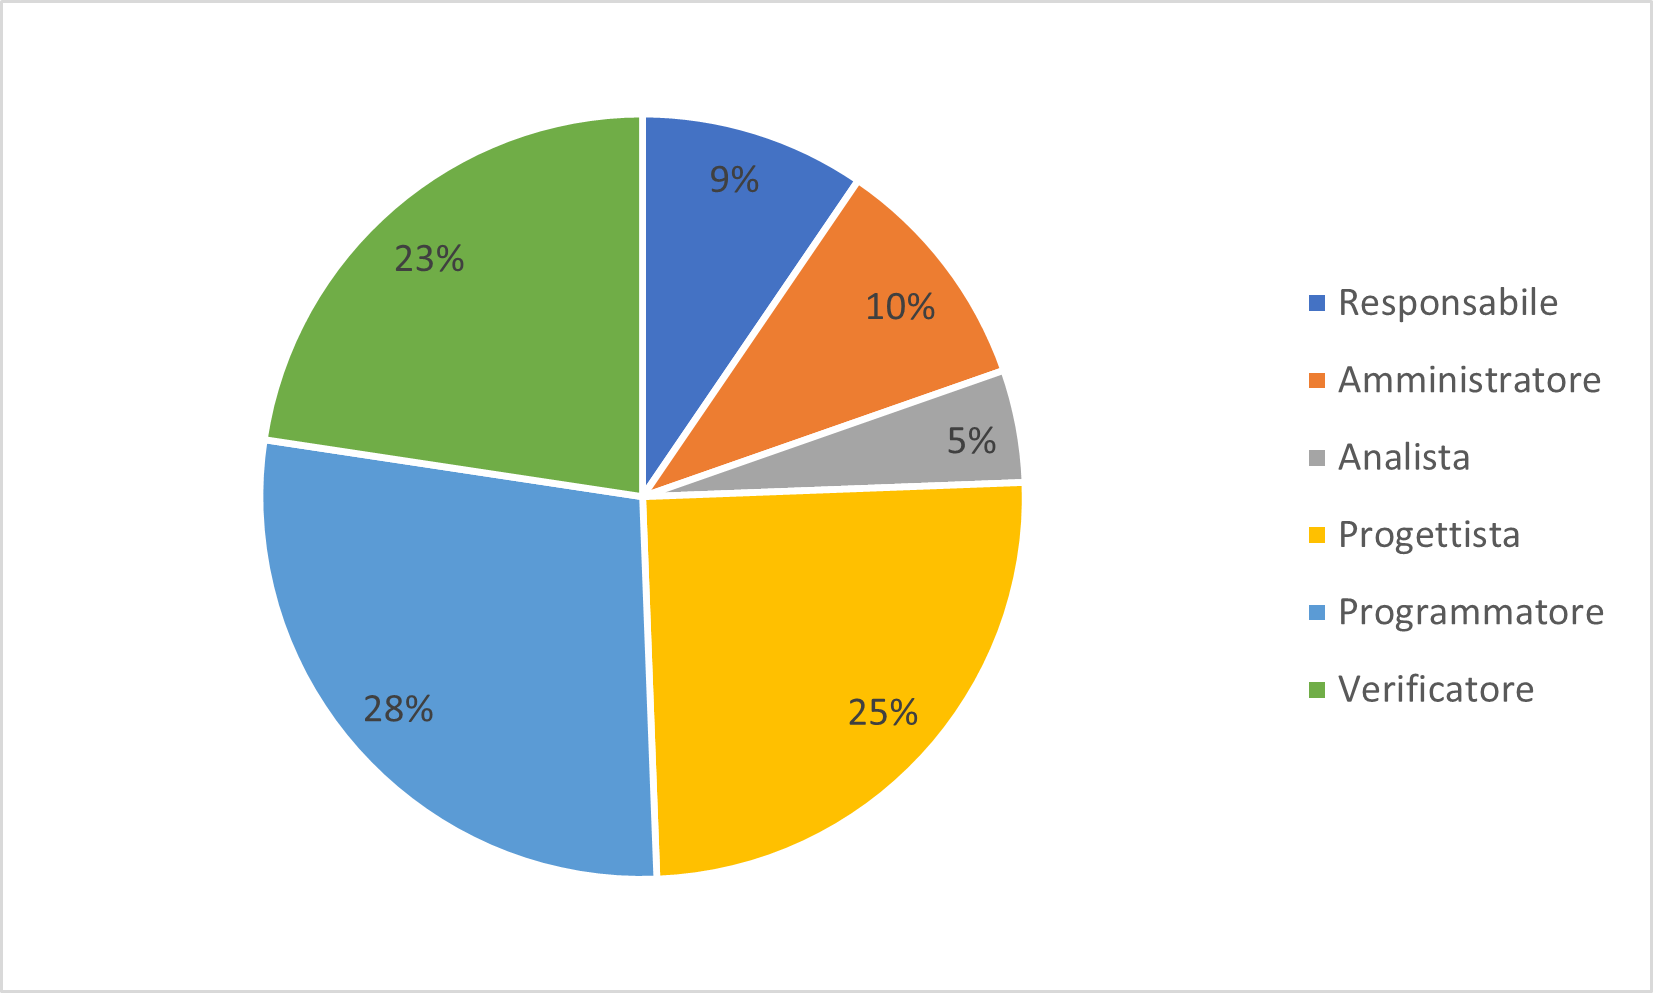
\includegraphics[width=0.8\linewidth]{res/images/preventivo/4-2.png}
	\caption{Diagramma percentuale ore/ruolo nella fase di Progettazione della proof of concept}
	\label{fig:diagramma costi ruolo fase progettazione della proof of concept}
\end{figure}

\subsection{Fase di progettazione completa e prima implementazione di base}
La fase è composta da quattro incrementi caratterizzati dalla distribuzione oraria descritta di seguito.

\subsubsection{IV incremento}
\paragraph{Prospetto orario}
Durante il IV incremento la distribuzione oraria sarà la seguente:

\rowcolors{1}{lightest-grayest}{blue!20}
\begin{longtable}{|l|c|c|c|c|c|c|c|}
	\hline
	\rowcolor{lighter-grayer}
	\textbf{Nome}     & \textbf{Re} & \textbf{Am} & \textbf{An} & \textbf{Pg} & \textbf{Pr} & \textbf{Ve} & \textbf{Totale} \\
	\hline
	\endfirsthead

	\hline
	Marco Canovese    & 2           & 0           & 0           & 5           & 0           & 0           & 7               \\
	\hline
	\hline
	Nicole Davanzo    & 0           & 0           & 0           & 0           & 5           & 2           & 7               \\
	\hline
	\hline
	Ivan Furlan       & 0           & 0           & 0           & 1           & 2           & 4           & 7               \\
	\hline
	\hline
	Gianmarco Guazzo  & 0           & 0           & 0           & 6           & 0           & 1           & 7               \\
	\hline
	\hline
	Stefano Lazzaroni & 1           & 0           & 0           & 3           & 1           & 2           & 7               \\
	\hline
	\hline
	Francesco Trolese & 2           & 0           & 0           & 0           & 1           & 4           & 7               \\
	\hline
	\hline
	Michele Veronesi  & 0           & 5           & 0           & 0           & 2           & 0           & 7               \\
	\hline
	\hline
	Totale            & 5           & 5          & 0          & 15           & 11           & 13           & 49              \\
	\hline
	\rowcolor{white}
	\caption{Tabella contenente il prospetto orario preventivato per il IV incremento}
\end{longtable}


La tabella può essere riassunta nel seguente istogramma:

\begin{figure}[H]
	\centering
	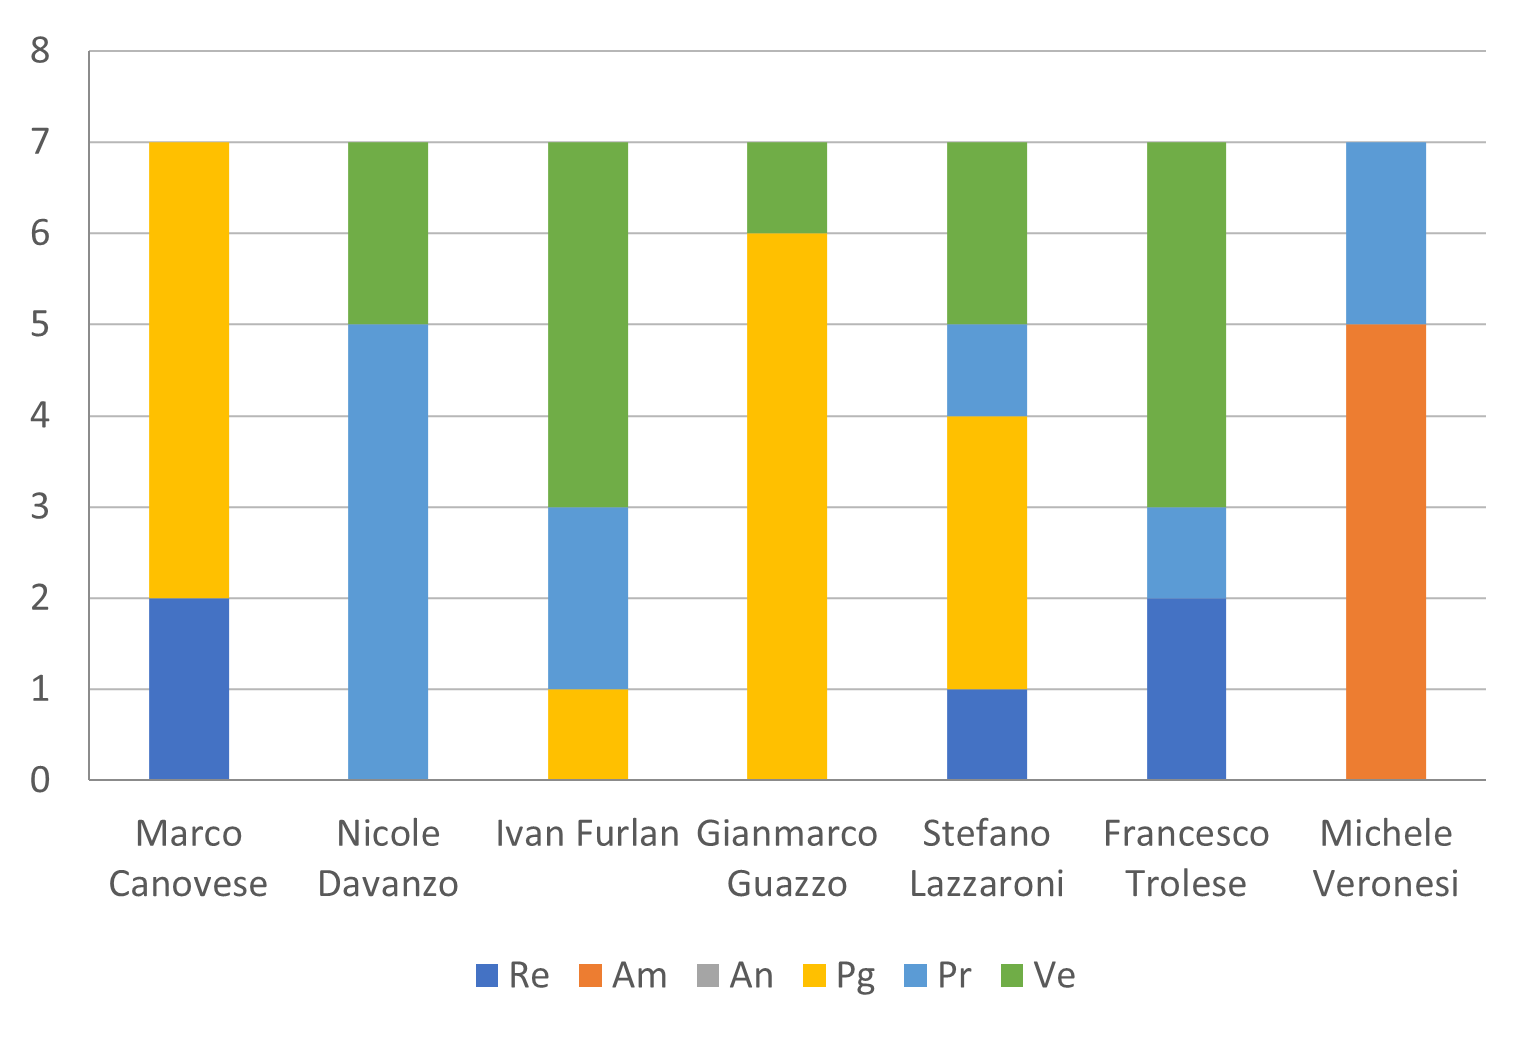
\includegraphics[width=0.8\linewidth]{res/images/preventivo/dettaglio_implementazione/1-1.png}
	\caption{Diagramma ore/ruolo componenti nel IV incremento}
	\label{fig:diagramma suddivisione ruoli IV incremento}
\end{figure}

\paragraph{Prospetto economico}
In base al prospetto orario, quello economico sarà il seguente:

\rowcolors{1}{lightest-grayest}{blue!20}
\begin{longtable}{|l|c|c|c|c|c|c|c|}
	\hline
	\rowcolor{lighter-grayer}
	\textbf{Ruolo}  & \textbf{Ore} & \textbf{Costo in €} \\
	\hline
	\endfirsthead

	\hline
	Responsabile    & 5            & 150,00              \\
	\hline
	\hline
	Amministratore  & 5           & 100,00              \\
	\hline
	\hline
	Analista        & 0           & 00,00              \\
	\hline
	\hline
	Progettista     & 15            & 330,00                   \\
	\hline
	\hline
	Programmatore   & 11            & 165,00                   \\
	\hline
	\hline
	Verificatore    & 13            & 195,00                   \\
	\hline
	\textbf{Totale} & 49           & 940,00            \\
	\hline
	\rowcolor{white}
	\caption{Tabella contenente il prospetto economico in riferimento al prospetto orario}
\end{longtable}
\pagebreak

La tabella può essere riassunta nel seguente areogramma:
\begin{figure}[H]
	\centering
	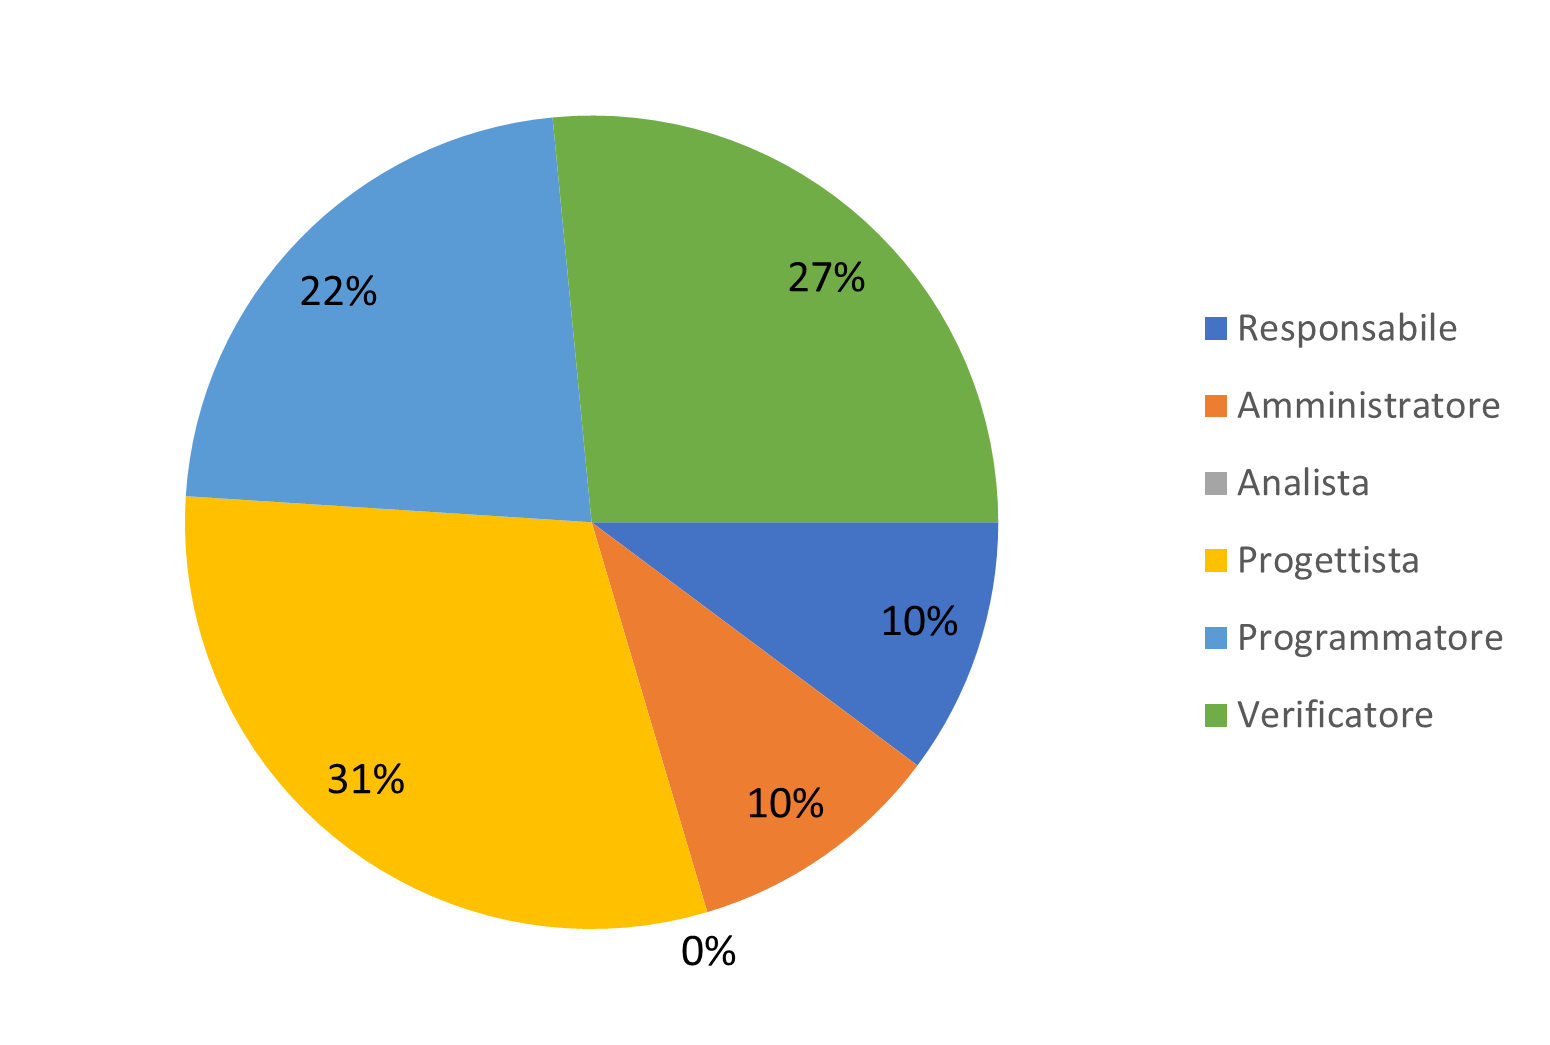
\includegraphics[width=0.8\linewidth]{res/images/preventivo/dettaglio_implementazione/1-2.png}
	\caption{Diagramma percentuale ore/ruolo nel IV incremento}
	\label{fig:diagramma costi ruolo  IV incremento}
\end{figure}

\subsubsection{V incremento}
\paragraph{Prospetto orario}
Durante il V incremento la distribuzione oraria sarà la seguente:

\rowcolors{1}{lightest-grayest}{blue!20}
\begin{longtable}{|l|c|c|c|c|c|c|c|}
	\hline
	\rowcolor{lighter-grayer}
	\textbf{Nome}     & \textbf{Re} & \textbf{Am} & \textbf{An} & \textbf{Pg} & \textbf{Pr} & \textbf{Ve} & \textbf{Totale} \\
	\hline
	\endfirsthead

	\hline
	Marco Canovese    & 0           & 0           & 0           & 0           & 4           & 0           & 4               \\
	\hline
	\hline
	Nicole Davanzo    & 2           & 0           & 0           & 0           & 3           & 1           & 4               \\
	\hline
	\hline
	Ivan Furlan       & 0           & 0           & 0           & 2           & 0           & 2           & 4               \\
	\hline
	\hline
	Gianmarco Guazzo  & 0           & 0           & 0           & 1           & 0           & 3           & 4               \\
	\hline
	\hline
	Stefano Lazzaroni & 0           & 0           & 0           & 1           & 0           & 3           & 4               \\
	\hline
	\hline
	Francesco Trolese & 0           & 0           & 0           & 2           & 0           & 2           & 4               \\
	\hline
	\hline
	Michele Veronesi  & 0           & 0           & 0           & 0           & 4           & 0           & 4               \\
	\hline
	\hline
	Totale            & 2          & 0          & 0          & 6           & 11           & 11          & 28              \\
	\hline
	\rowcolor{white}
	\caption{Tabella contenente il prospetto orario preventivato per il V incremento}
\end{longtable}


La tabella può essere riassunta nel seguente istogramma:

\begin{figure}[H]
	\centering
	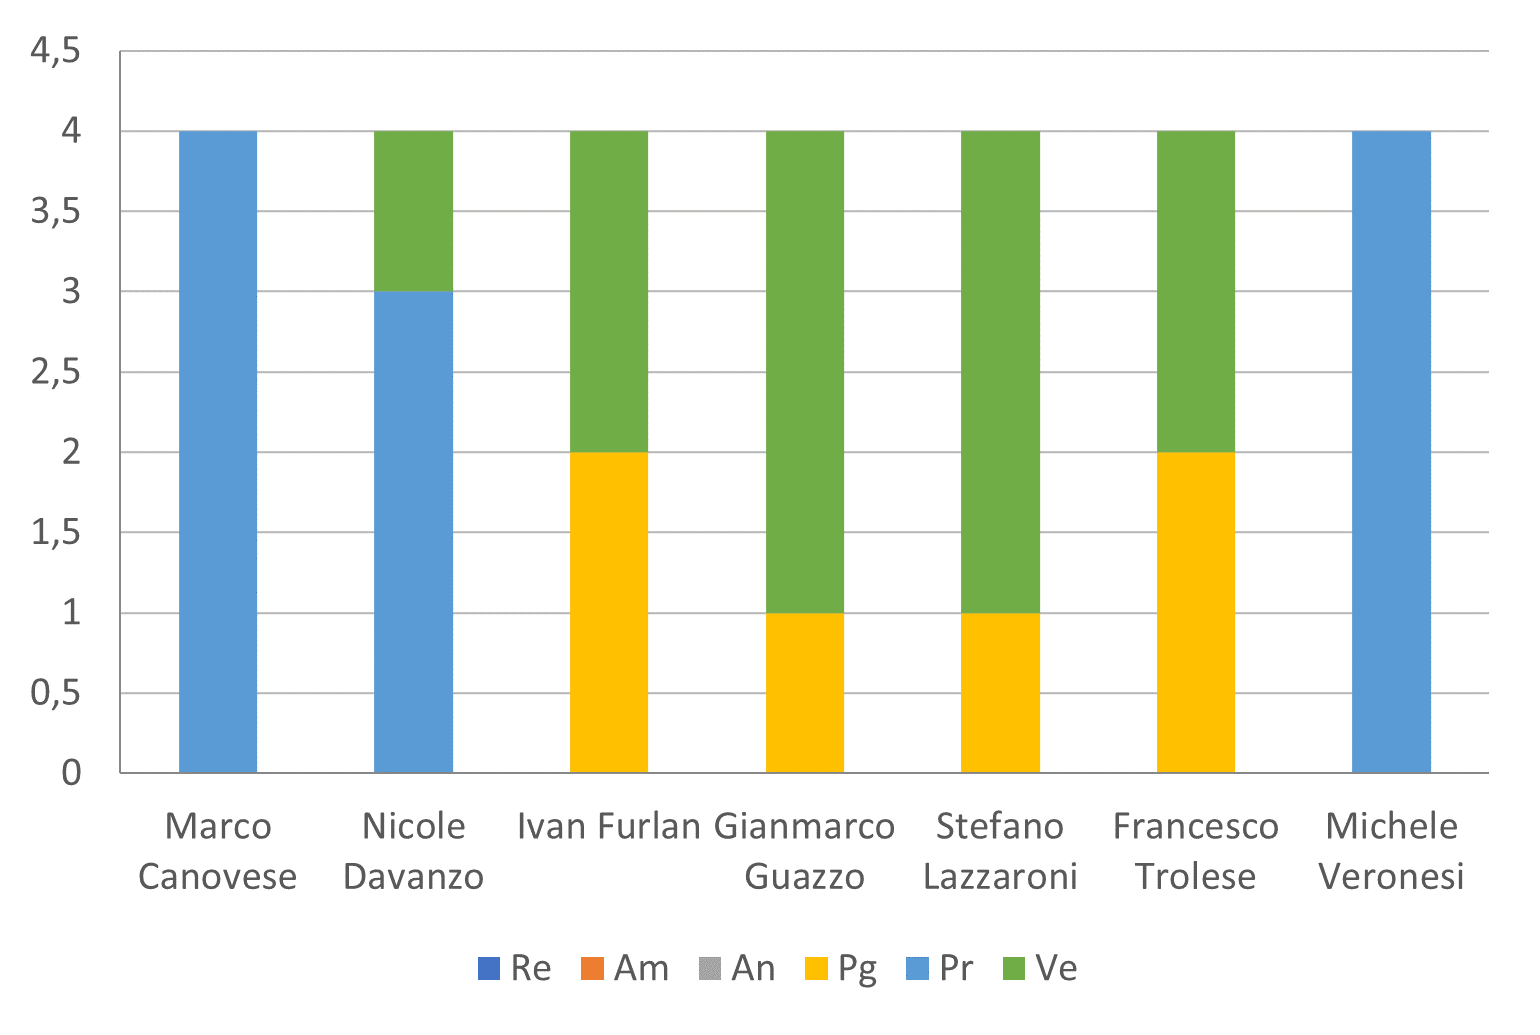
\includegraphics[width=0.8\linewidth]{res/images/preventivo/dettaglio_implementazione/2-1.png}
	\caption{Diagramma ore/ruolo componenti nel V incremento}
	\label{fig:diagramma suddivisione ruoli V incremento}
\end{figure}

\paragraph{Prospetto economico}
In base al prospetto orario, quello economico sarà il seguente:

\rowcolors{1}{lightest-grayest}{blue!20}
\begin{longtable}{|l|c|c|c|c|c|c|c|}
	\hline
	\rowcolor{lighter-grayer}
	\textbf{Ruolo}  & \textbf{Ore} & \textbf{Costo in €} \\
	\hline
	\endfirsthead

	\hline
	Responsabile    & 2            & 60,00              \\
	\hline
	\hline
	Amministratore  & 0           & 00,00              \\
	\hline
	\hline
	Analista        & 0           & 00,00              \\
	\hline
	\hline
	Progettista     & 6            & 132,00                   \\
	\hline
	\hline
	Programmatore   & 11            & 165,00                   \\
	\hline
	\hline
	Verificatore    & 11           & 165,00              \\
	\hline
	\hline
	\textbf{Totale} & 28           & 462,00            \\
	\hline
	\rowcolor{white}
	\caption{Tabella contenente il prospetto economico in riferimento al prospetto orario}
\end{longtable}
\pagebreak

La tabella può essere riassunta nel seguente areogramma:
\begin{figure}[H]
	\centering
	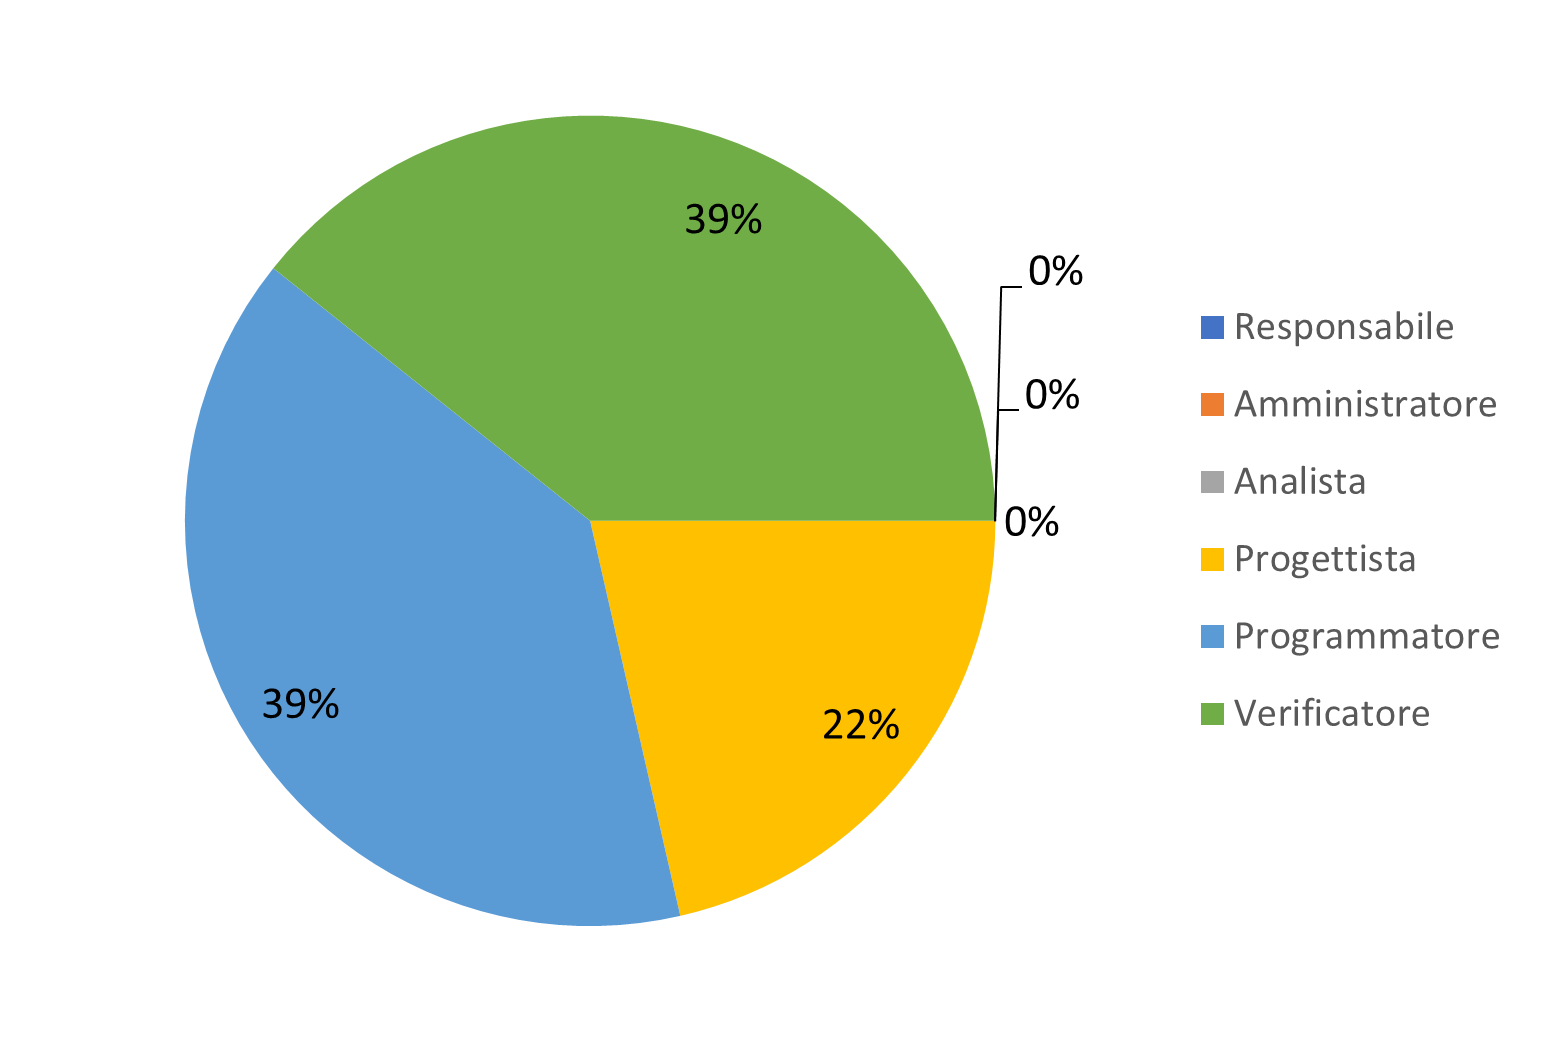
\includegraphics[width=0.8\linewidth]{res/images/preventivo/dettaglio_implementazione/2-2.png}
	\caption{Diagramma percentuale ore/ruolo nel V incremento}
	\label{fig:diagramma costi ruolo V incremento}
\end{figure}

\subsubsection{VI incremento}
\paragraph{Prospetto orario}
Durante il VI incremento la distribuzione oraria sarà la seguente:

\rowcolors{1}{lightest-grayest}{blue!20}
\begin{longtable}{|l|c|c|c|c|c|c|c|}
	\hline
	\rowcolor{lighter-grayer}
	\textbf{Nome}     & \textbf{Re} & \textbf{Am} & \textbf{An} & \textbf{Pg} & \textbf{Pr} & \textbf{Ve} & \textbf{Totale} \\
	\hline
	\endfirsthead

	\hline
	Marco Canovese    & 0           & 0           & 0           & 0           & 0           & 4           & 4               \\
	\hline
	\hline
	Nicole Davanzo    & 0           & 0           & 0           & 0           & 4           & 0           & 4               \\
	\hline
	\hline
	Ivan Furlan       & 0           & 0           & 0           & 4           & 0           & 0           & 4               \\
	\hline
	\hline
	Gianmarco Guazzo  & 0           & 0           & 4           & 0           & 0           & 0           & 4               \\
	\hline
	\hline
	Stefano Lazzaroni & 1           & 0           & 0           & 1           & 2           & 0           & 4               \\
	\hline
	\hline
	Francesco Trolese & 0           & 0           & 0           & 4           & 0           & 0           & 4               \\
	\hline
	\hline
	Michele Veronesi  & 0           & 2           & 0           & 0           & 2           & 0           & 4               \\
	\hline
	\hline
	Totale            & 1           & 2           & 4          & 9           & 8           & 4          & 28              \\
	\hline
	\rowcolor{white}
	\caption{Tabella contenente il prospetto orario preventivato per il VI incremento}
\end{longtable}


La tabella può essere riassunta nel seguente istogramma:

\begin{figure}[H]
	\centering
	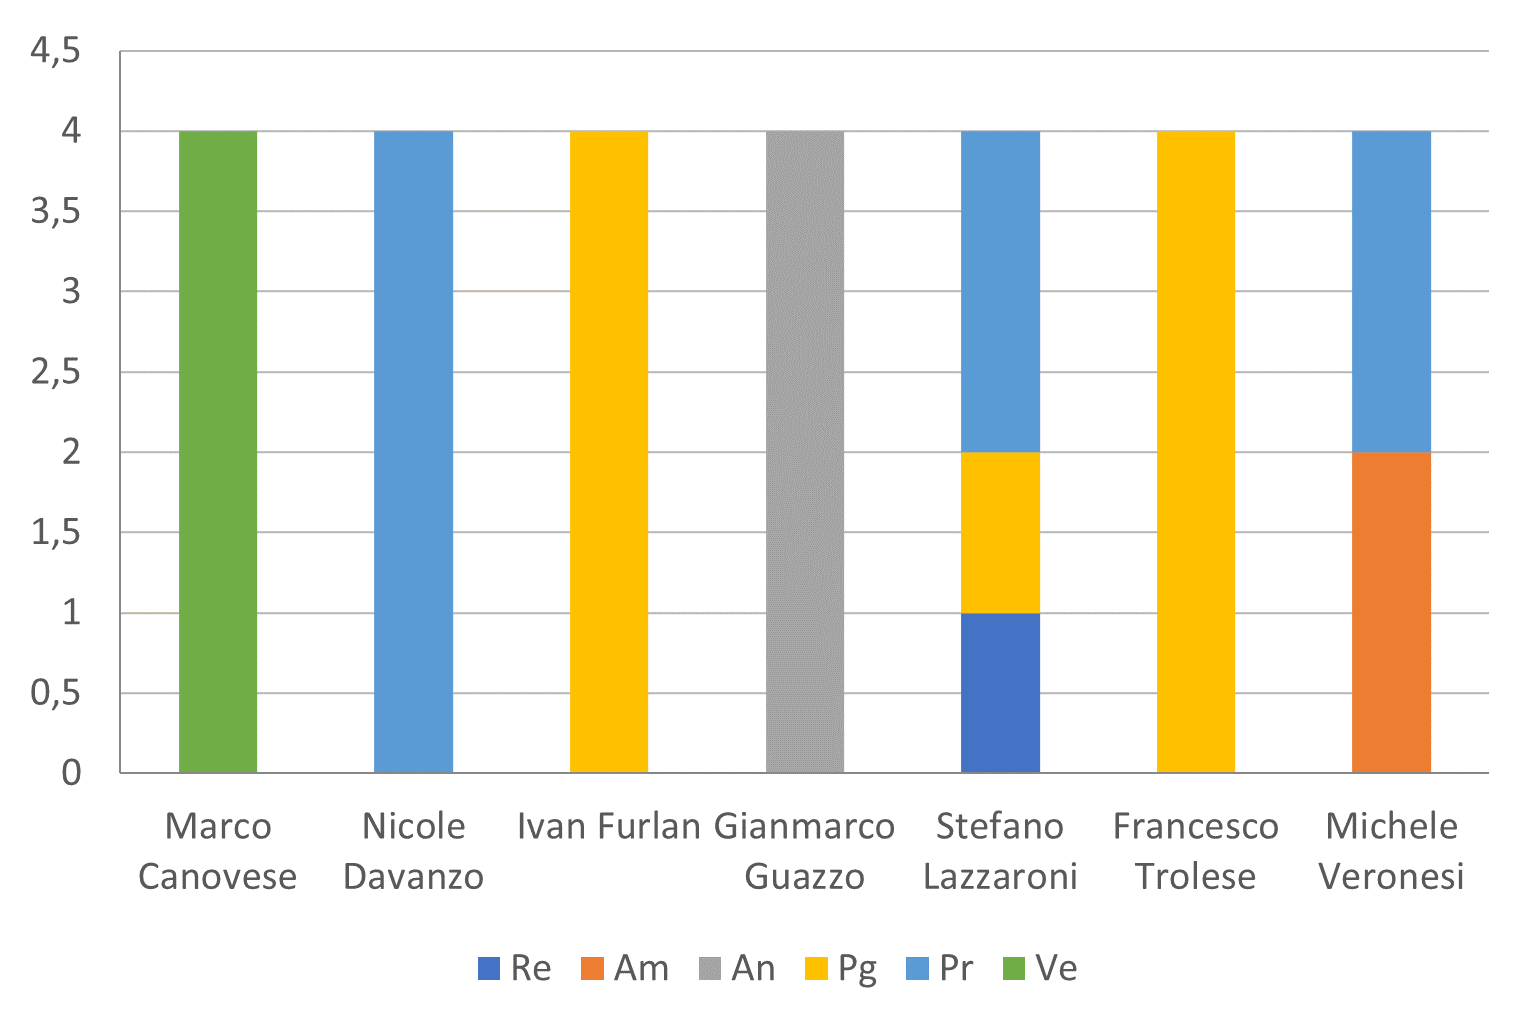
\includegraphics[width=0.8\linewidth]{res/images/preventivo/dettaglio_implementazione/3-1.png}
	\caption{Diagramma ore/ruolo componenti nel VI incremento}
	\label{fig:diagramma suddivisione ruoli VI incremento}
\end{figure}

\paragraph{Prospetto economico}
In base al prospetto orario, quello economico sarà il seguente:

\rowcolors{1}{lightest-grayest}{blue!20}
\begin{longtable}{|l|c|c|c|c|c|c|c|}
	\hline
	\rowcolor{lighter-grayer}
	\textbf{Ruolo}  & \textbf{Ore} & \textbf{Costo in €} \\
	\hline
	\endfirsthead

	\hline
	Responsabile    & 1            & 30,00              \\
	\hline
	\hline
	Amministratore  & 2            & 40,00               \\
	\hline
	\hline
	Analista        & 4           & 100,00              \\
	\hline
	\hline
	Progettista     & 9            & 198,00                   \\
	\hline
	\hline
	Programmatore   & 8            & 120,00                   \\
	\hline
	\hline
	Verificatore    & 4           & 60,00              \\
	\hline
	\textbf{Totale} & 28           & 548,00            \\
	\hline
	\rowcolor{white}
	\caption{Tabella contenente il prospetto economico in riferimento al prospetto orario}
\end{longtable}
\pagebreak

La tabella può essere riassunta nel seguente areogramma:
\begin{figure}[H]
	\centering
	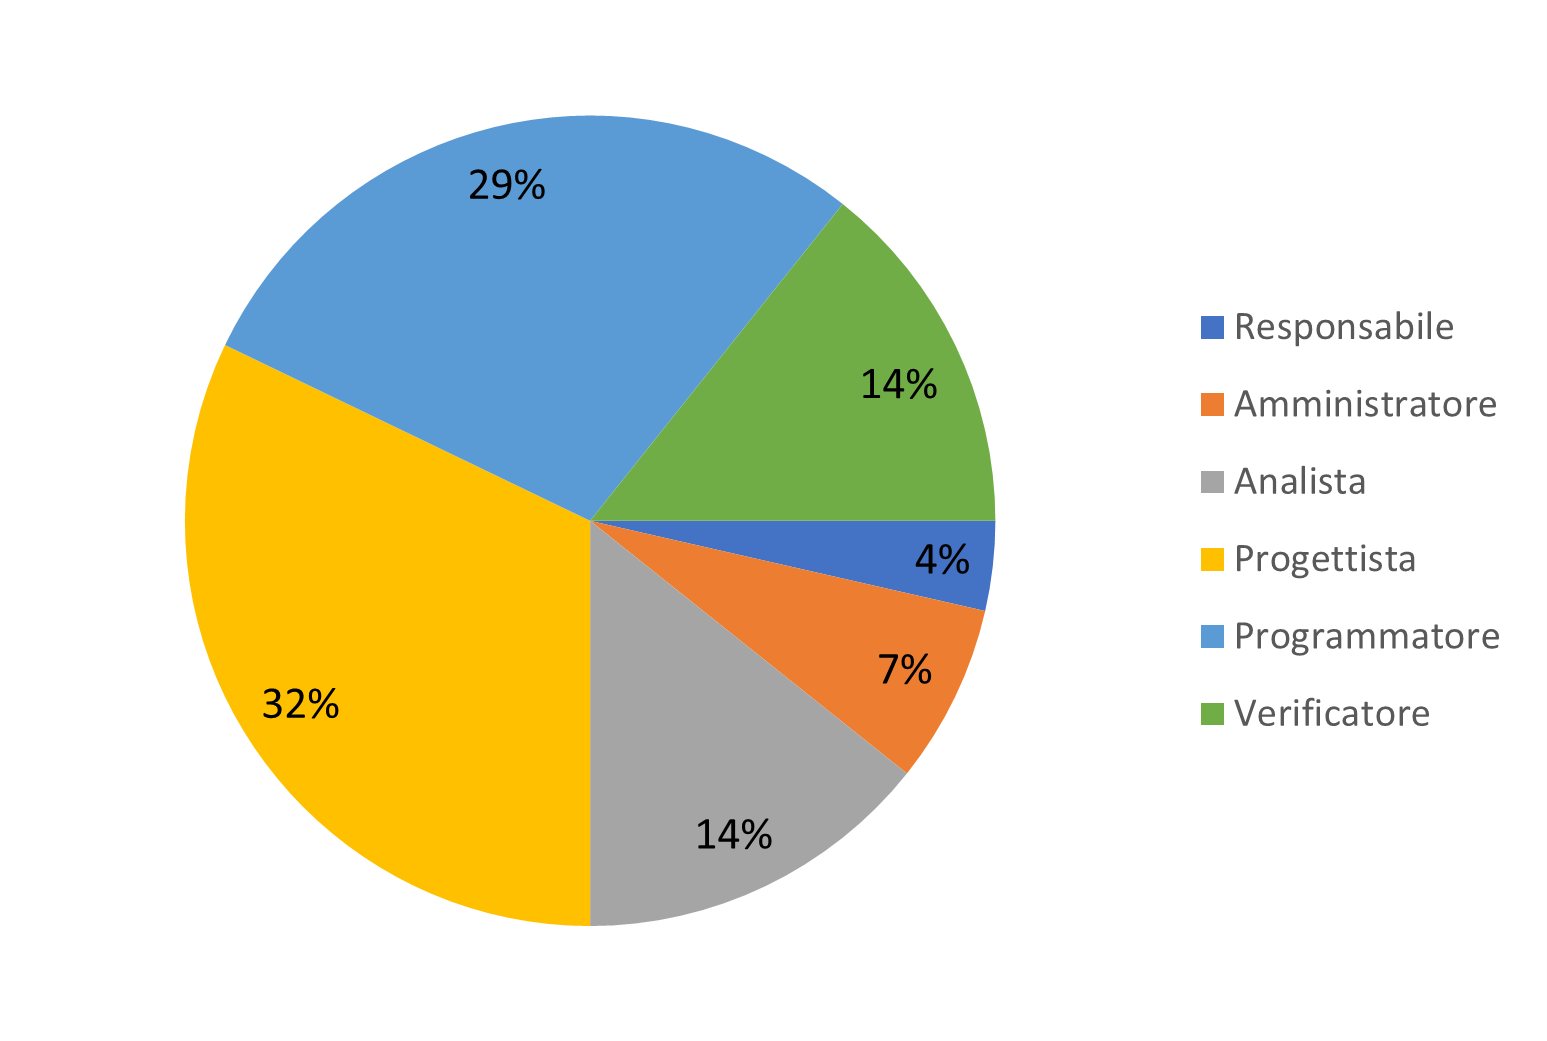
\includegraphics[width=0.8\linewidth]{res/images/preventivo/dettaglio_implementazione/3-2.png}
	\caption{Diagramma percentuale ore/ruolo nel VI incremento}
	\label{fig:diagramma costi ruolo VI incremento}
\end{figure}

\subsubsection{VII incremento}
\paragraph{Prospetto orario}
Durante il VII incremento la distribuzione oraria sarà la seguente:

\rowcolors{1}{lightest-grayest}{blue!20}
\begin{longtable}{|l|c|c|c|c|c|c|c|}
	\hline
	\rowcolor{lighter-grayer}
	\textbf{Nome}     & \textbf{Re} & \textbf{Am} & \textbf{An} & \textbf{Pg} & \textbf{Pr} & \textbf{Ve} & \textbf{Totale} \\
	\hline
	\endfirsthead

	\hline
	Marco Canovese    & 0           & 0           & 2           & 0           & 5           & 0           & 7               \\
	\hline
	\hline
	Nicole Davanzo    & 0           & 0           & 0           & 0           & 0           & 7           & 7               \\
	\hline
	\hline
	Ivan Furlan       & 0           & 0           & 0           & 0           & 4           & 3           & 7               \\
	\hline
	\hline
	Gianmarco Guazzo  & 0           & 0           & 0           & 2           & 4           & 1           & 7               \\
	\hline
	\hline
	Stefano Lazzaroni & 0           & 2           & 0           & 0           & 0           & 5           & 7               \\
	\hline
	\hline
	Francesco Trolese & 2           & 2           & 0           & 0           & 2           & 1           & 7               \\
	\hline
	\hline
	Michele Veronesi  & 0           & 0           & 0           & 3           & 4           & 0           & 7               \\
	\hline
	\hline
	Totale            & 2           & 4           & 2          & 5           & 19           & 17          & 49              \\
	\hline
	\rowcolor{white}
	\caption{Tabella contenente il prospetto orario preventivato per il VII incremento}
\end{longtable}


La tabella può essere riassunta nel seguente istogramma:

\begin{figure}[H]
	\centering
	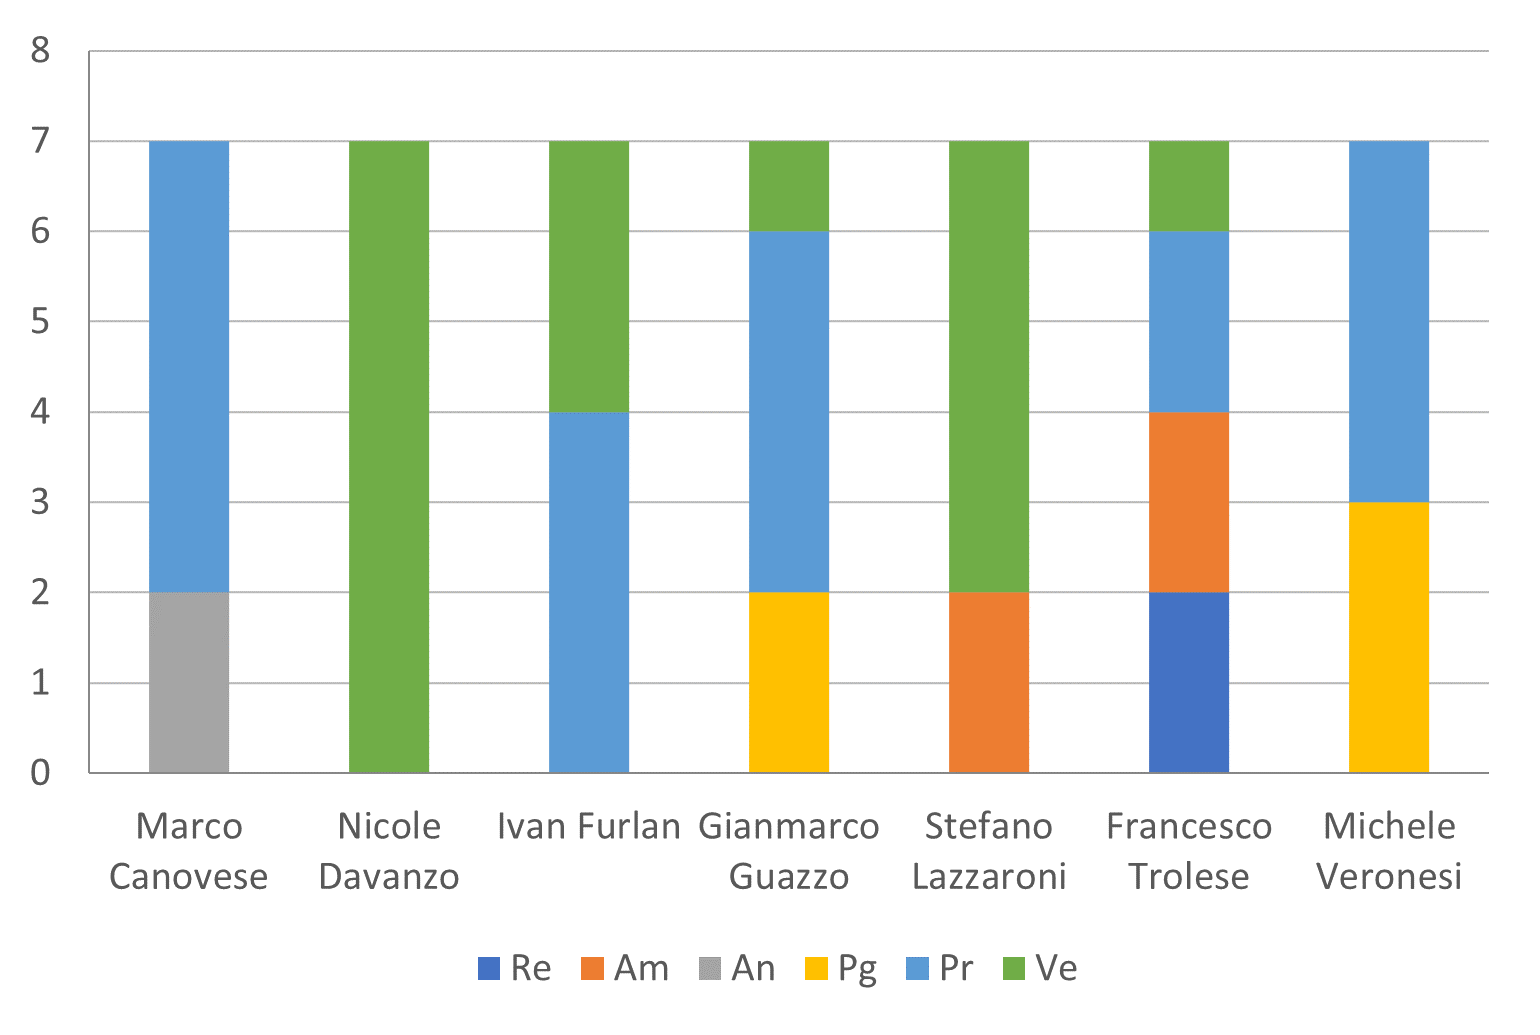
\includegraphics[width=0.8\linewidth]{res/images/preventivo/dettaglio_implementazione/4-1.png}
	\caption{Diagramma ore/ruolo componenti nel VII incremento}
	\label{fig:diagramma suddivisione ruoli VII incremento}
\end{figure}

\paragraph{Prospetto economico}
In base al prospetto orario, quello economico sarà il seguente:

\rowcolors{1}{lightest-grayest}{blue!20}
\begin{longtable}{|l|c|c|c|c|c|c|c|}
	\hline
	\rowcolor{lighter-grayer}
	\textbf{Ruolo}  & \textbf{Ore} & \textbf{Costo in €} \\
	\hline
	\endfirsthead

	\hline
	Responsabile    & 2            & 60,00              \\
	\hline
	\hline
	Amministratore  & 4            & 80,00               \\
	\hline
	\hline
	Analista        & 2           & 50,00              \\
	\hline
	\hline
	Progettista     & 5            & 110,00                   \\
	\hline
	\hline
	Programmatore   & 19            & 285,00                   \\
	\hline
	\hline
	Verificatore    & 17           & 255,00              \\
	\hline
	\textbf{Totale} & 49           & 840,00            \\
	\hline
	\rowcolor{white}
	\caption{Tabella contenente il prospetto economico in riferimento al prospetto orario}
\end{longtable}
\pagebreak

La tabella può essere riassunta nel seguente areogramma:
\begin{figure}[H]
	\centering
	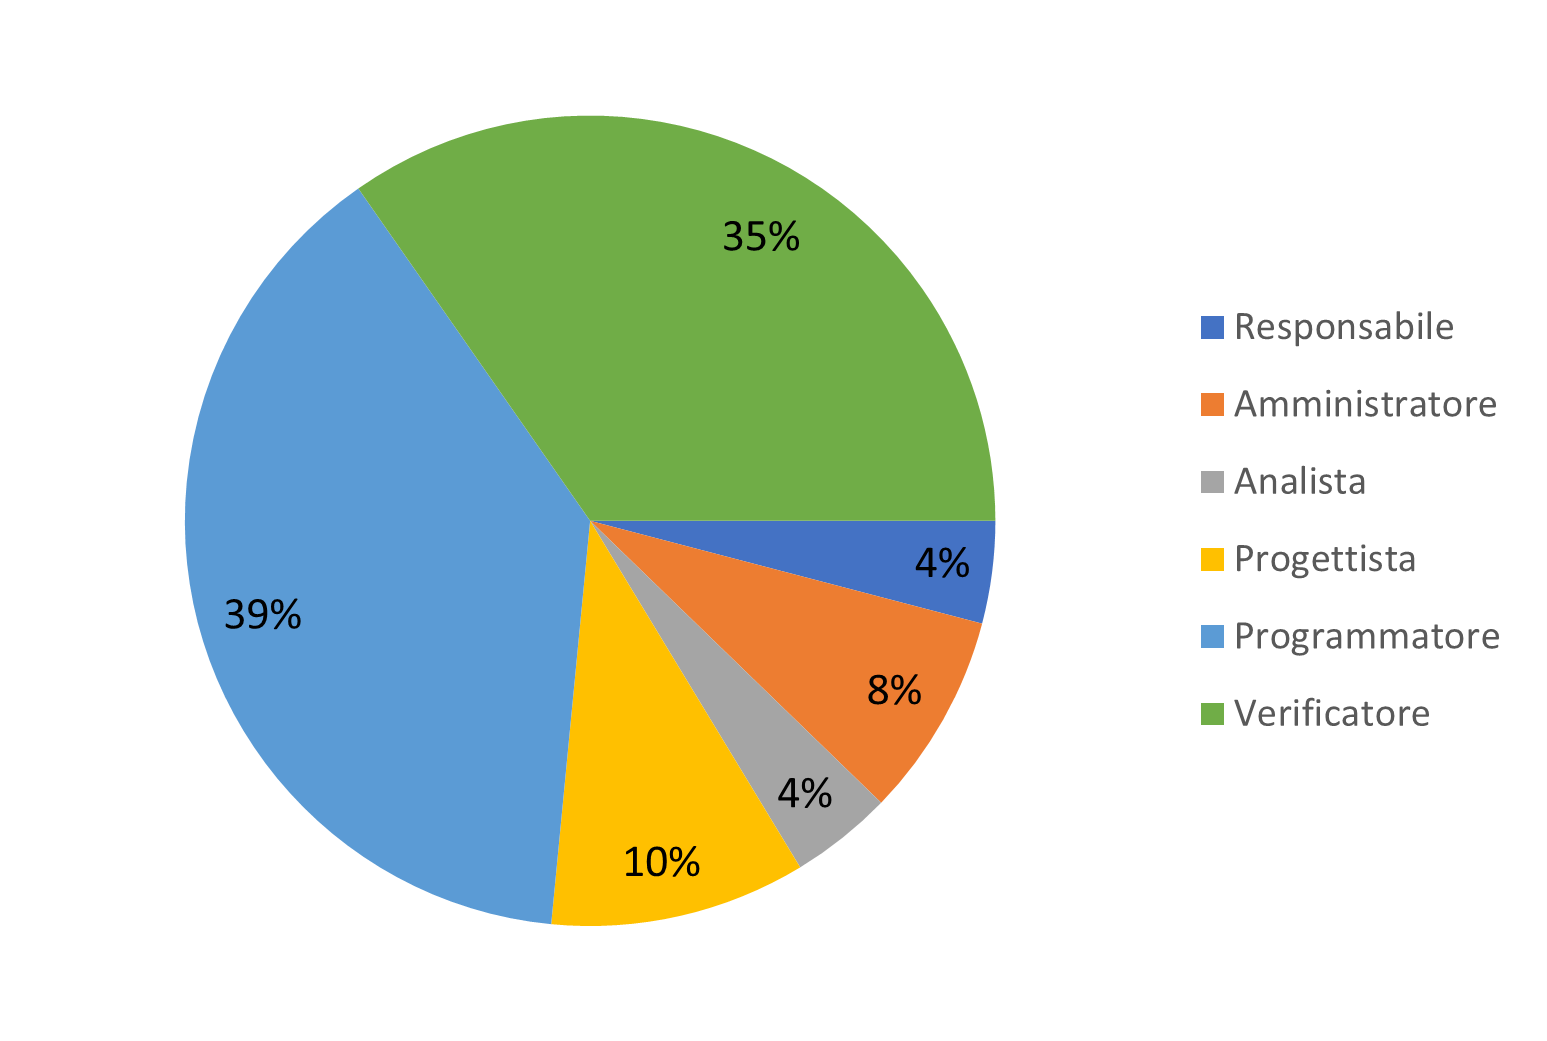
\includegraphics[width=0.8\linewidth]{res/images/preventivo/dettaglio_implementazione/4-2.png}
	\caption{Diagramma percentuale ore/ruolo nel VII incremento}
	\label{fig:diagramma costi ruolo VII incremento}
\end{figure}

\subsubsection{Fase complessiva}
\paragraph{Prospetto orario}
Durante la fase di progettazione completa e prima implementazione di base la distribuzione oraria sarà la seguente:

\rowcolors{1}{lightest-grayest}{blue!20}
\begin{longtable}{|l|c|c|c|c|c|c|c|}
	\hline
	\rowcolor{lighter-grayer}
	\textbf{Nome}     & \textbf{Re} & \textbf{Am} & \textbf{An} & \textbf{Pg} & \textbf{Pr} & \textbf{Ve} & \textbf{Totale} \\
	\hline
	\endfirsthead

	\hline
	Marco Canovese    & 2           & 0           & 2           & 8           & 10          & 4           & 26              \\
	\hline
	\hline
	Nicole Davanzo    & 0           & 0           & 0           & 3           & 13          & 10          & 26              \\
	\hline
	\hline
	Ivan Furlan       & 0           & 0           & 0           & 10          & 7           & 9           & 26              \\
	\hline
	\hline
	Gianmarco Guazzo  & 0           & 0           & 0           & 12          & 9           & 5           & 26              \\
	\hline
	\hline
	Stefano Lazzaroni & 2           & 2           & 0           & 8           & 4           & 10          & 26              \\
	\hline
	\hline
	Francesco Trolese & 4           & 2           & 0           & 9           & 4           & 7           & 26              \\
	\hline
	\hline
	Michele Veronesi  & 0           & 7           & 0           & 6           & 13          & 0           & 26              \\
	\hline
	\hline
	Totale            & 8           & 11          & 2           & 56          & 60          & 45          & 182             \\
	\hline
	\rowcolor{white}
	\caption{Tabella contenente il prospetto orario preventivato per la fase di progettazione completa e prima implementazione di base}
\end{longtable}


La tabella può essere riassunta nel seguente istogramma:

\begin{figure}[H]
	\centering
	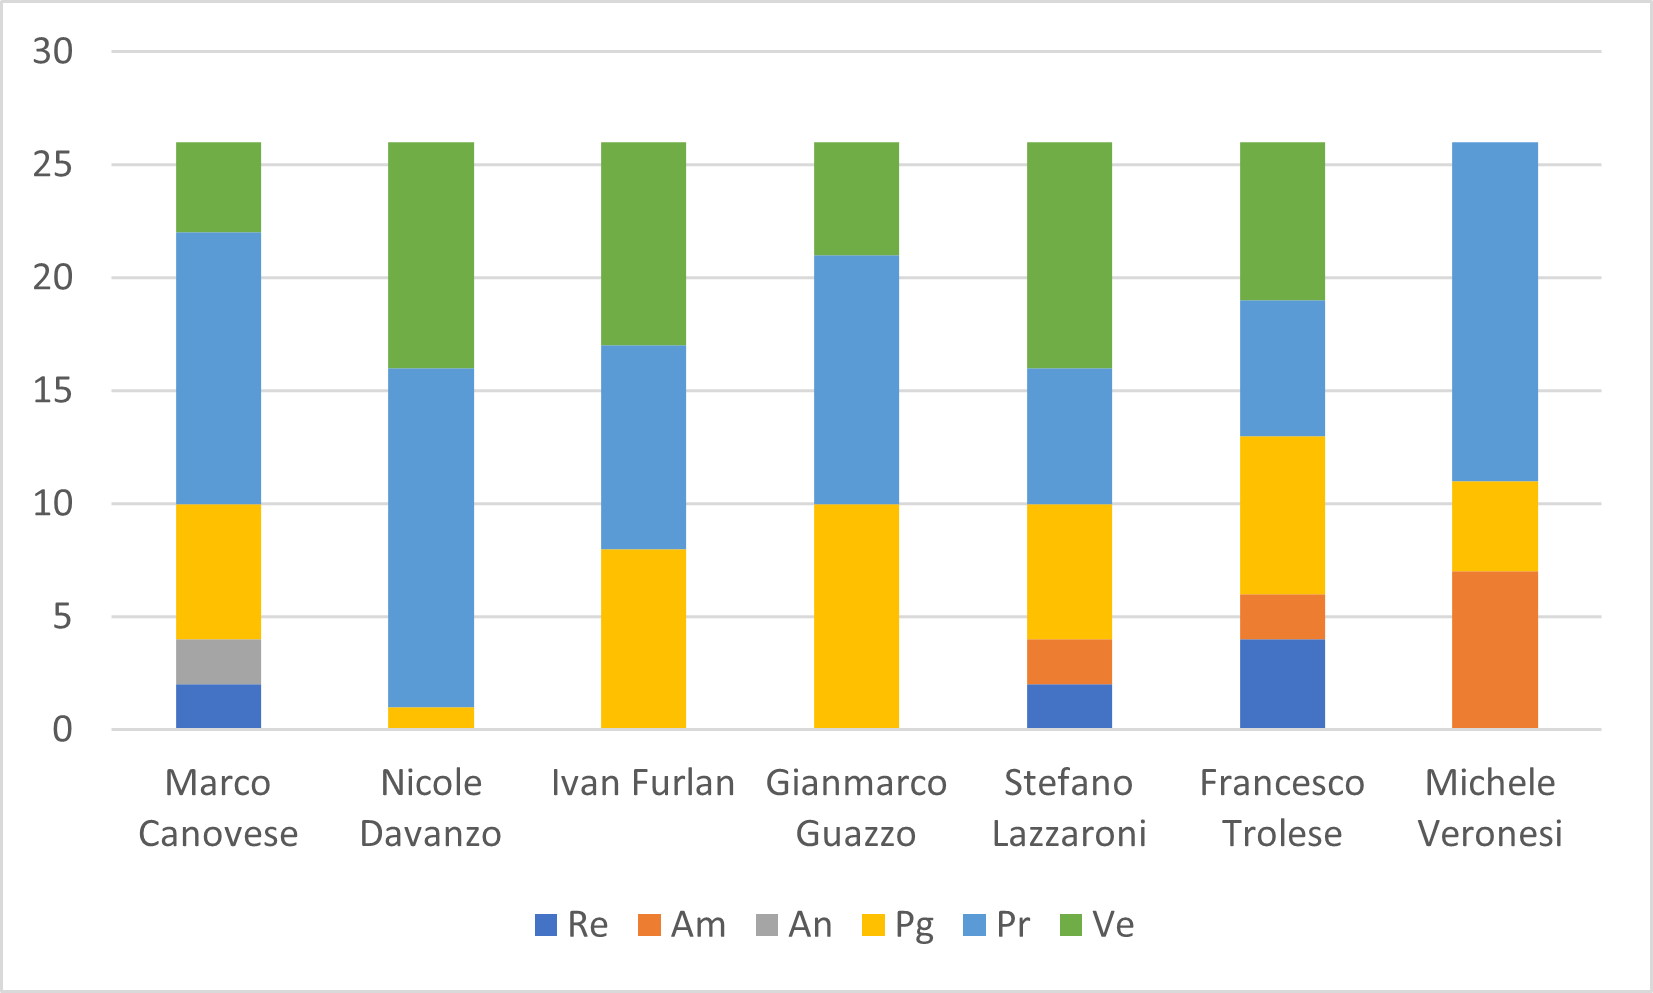
\includegraphics[width=0.8\linewidth]{res/images/preventivo/5-1.png}
	\caption{Diagramma ore/ruolo componenti nella fase di Progettazione completa e prima implementazione di base}
	\label{fig:diagramma suddivisione ruoli fase progettazione completa e prima implementazione di base}
\end{figure}

\paragraph{Prospetto economico}
In base al prospetto orario, quello economico sarà il seguente:

\rowcolors{1}{lightest-grayest}{blue!20}
\begin{longtable}{|l|c|c|c|c|c|c|c|}
	\hline
	\rowcolor{lighter-grayer}
	\textbf{Ruolo}  & \textbf{Ore} & \textbf{Costo in €} \\
	\hline
	\endfirsthead

	\hline
	Responsabile    & 8            & 240,00              \\
	\hline
	\hline
	Amministratore  & 11           & 220,00              \\
	\hline
	\hline
	Analista        & 2            & 50,00               \\
	\hline
	\hline
	Progettista     & 56           & 1232,00             \\
	\hline
	\hline
	Programmatore   & 60           & 900,00              \\
	\hline
	\hline
	Verificatore    & 45           & 675,00              \\
	\hline
	\hline
	\textbf{Totale} & 182          & 3.317,00            \\
	\hline
	\rowcolor{white}
	\caption{Tabella contenente il prospetto economico in riferimento al prospetto orario}
\end{longtable}
\pagebreak

La tabella può essere riassunta nel seguente areogramma:
\begin{figure}[H]
	\centering
	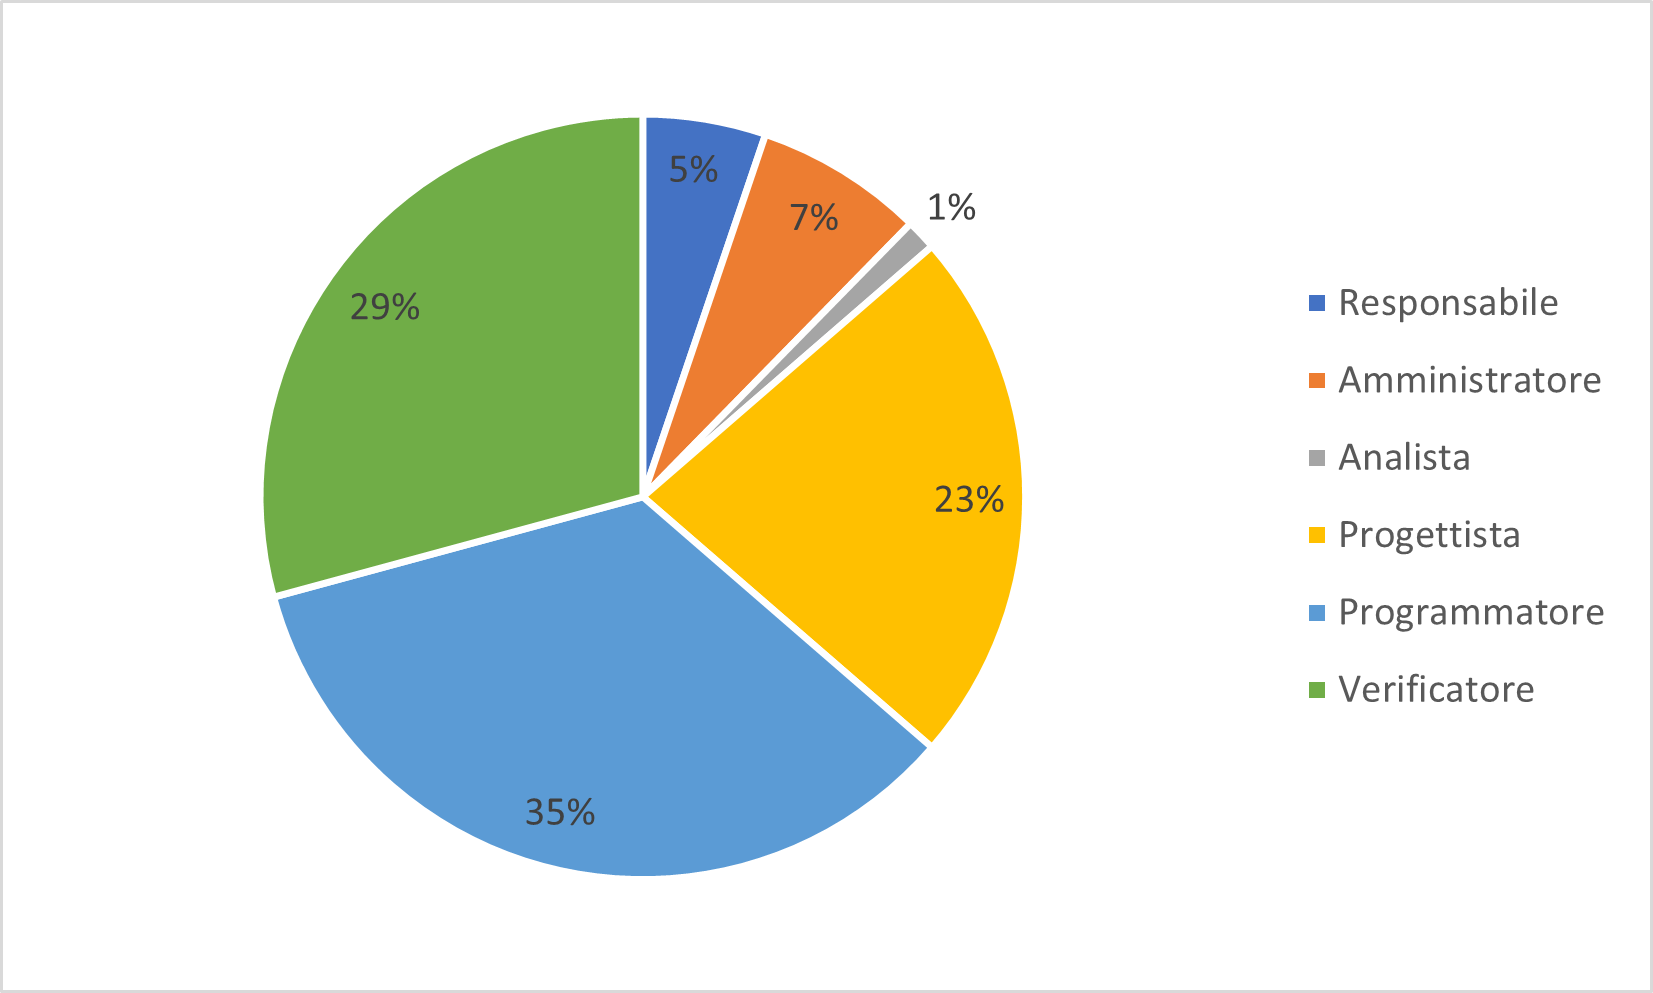
\includegraphics[width=0.8\linewidth]{res/images/preventivo/5-2.png}
	\caption{Diagramma percentuale ore/ruolo nella fase di Progettazione completa e prima implementazione di base}
	\label{fig:diagramma costi ruolo fase progettazione completa e prima implementazione di base}
\end{figure}

\subsection{Termine implementazione e raffinamento generale}
La fase è composta da due incrementi caratterizzati dalla distribuzione oraria descritta di seguito.

\subsubsection{VIII incremento}
\paragraph{Prospetto orario}
Durante il VIII incremento la distribuzione oraria sarà la seguente:

\rowcolors{1}{lightest-grayest}{blue!20}
\begin{longtable}{|l|c|c|c|c|c|c|c|}
	\hline
	\rowcolor{lighter-grayer}
	\textbf{Nome}     & \textbf{Re} & \textbf{Am} & \textbf{An} & \textbf{Pg} & \textbf{Pr} & \textbf{Ve} & \textbf{Totale} \\
	\hline
	\endfirsthead

	\hline
	Marco Canovese    & 0           & 0           & 0           & 6           & 6           & 8           & 20               \\
	\hline
	\hline
	Nicole Davanzo    & 1           & 3           & 0           & 6           & 4           & 6           & 20            \\
	\hline
	\hline
	Ivan Furlan       & 0           & 2           & 0           & 6           & 7           & 5           & 20               \\
	\hline
	\hline
	Gianmarco Guazzo  & 2           & 0           & 0           & 4           & 7           & 7           & 20               \\
	\hline
	\hline
	Stefano Lazzaroni & 0           & 0           & 0           & 7           & 7           & 6           & 20               \\
	\hline
	\hline
	Francesco Trolese & 0           & 0           & 0           & 5           & 8           & 7           & 20               \\
	\hline
	\hline
	Michele Veronesi  & 2           & 0           & 0           & 8           & 2           & 8           & 20               \\
	\hline
	\hline
	Totale            & 5           & 5          & 0          & 42           & 41           & 47           & 140              \\
	\hline
	\rowcolor{white}
	\caption{Tabella contenente il prospetto orario preventivato per il VIII incremento}
\end{longtable}


La tabella può essere riassunta nel seguente istogramma:

\begin{figure}[H]
	\centering
	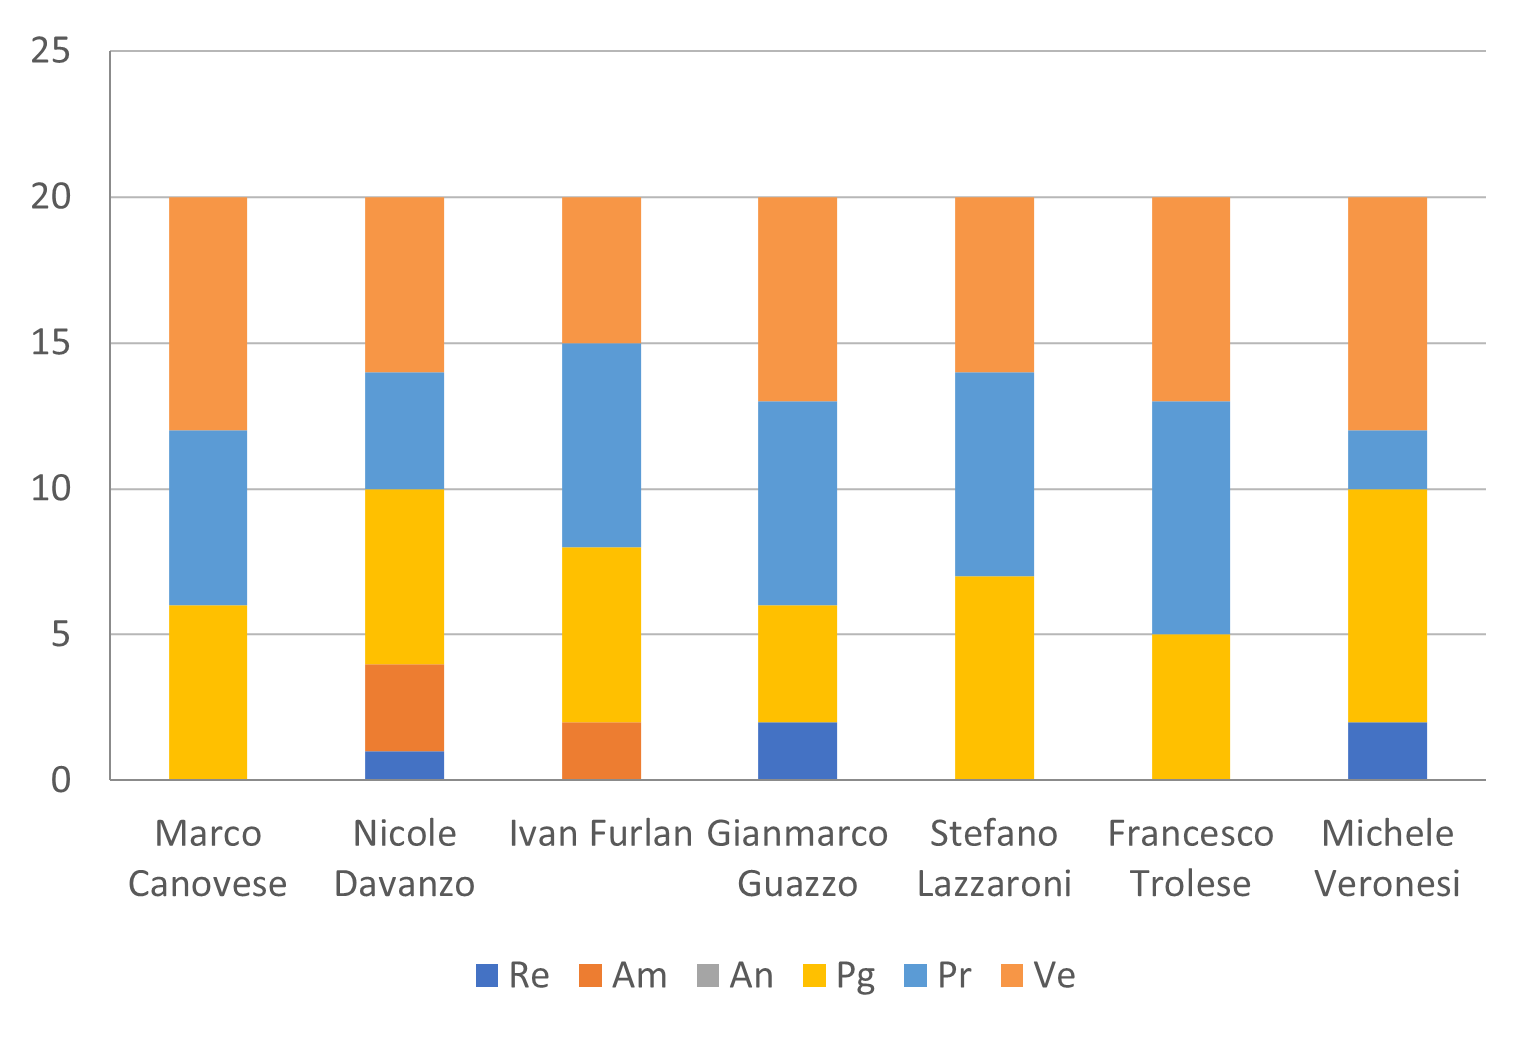
\includegraphics[width=0.8\linewidth]{res/images/preventivo/dettaglio_termineimp/1-1.png}
	\caption{Diagramma ore/ruolo componenti nel VIII incremento}
	\label{fig:diagramma suddivisione ruoli VIII incremento}
\end{figure}

\paragraph{Prospetto economico}
In base al prospetto orario, quello economico sarà il seguente:

\rowcolors{1}{lightest-grayest}{blue!20}
\begin{longtable}{|l|c|c|c|c|c|c|c|}
	\hline
	\rowcolor{lighter-grayer}
	\textbf{Ruolo}  & \textbf{Ore} & \textbf{Costo in €} \\
	\hline
	\endfirsthead

	\hline
	Responsabile    & 5            & 150,00              \\
	\hline
	\hline
	Amministratore  & 5           & 100,00              \\
	\hline
	\hline
	Analista        & 0           & 00,00              \\
	\hline
	\hline
	Progettista     & 42            & 924,00                   \\
	\hline
	\hline
	Programmatore   & 41            & 615,00                   \\
	\hline
	\hline
	Verificatore    & 47            & 705,00                   \\
	\hline
	\textbf{Totale} & 140           & 2.494,00            \\
	\hline
	\rowcolor{white}
	\caption{Tabella contenente il prospetto economico in riferimento al prospetto orario}
\end{longtable}
\pagebreak

La tabella può essere riassunta nel seguente areogramma:
\begin{figure}[H]
	\centering
	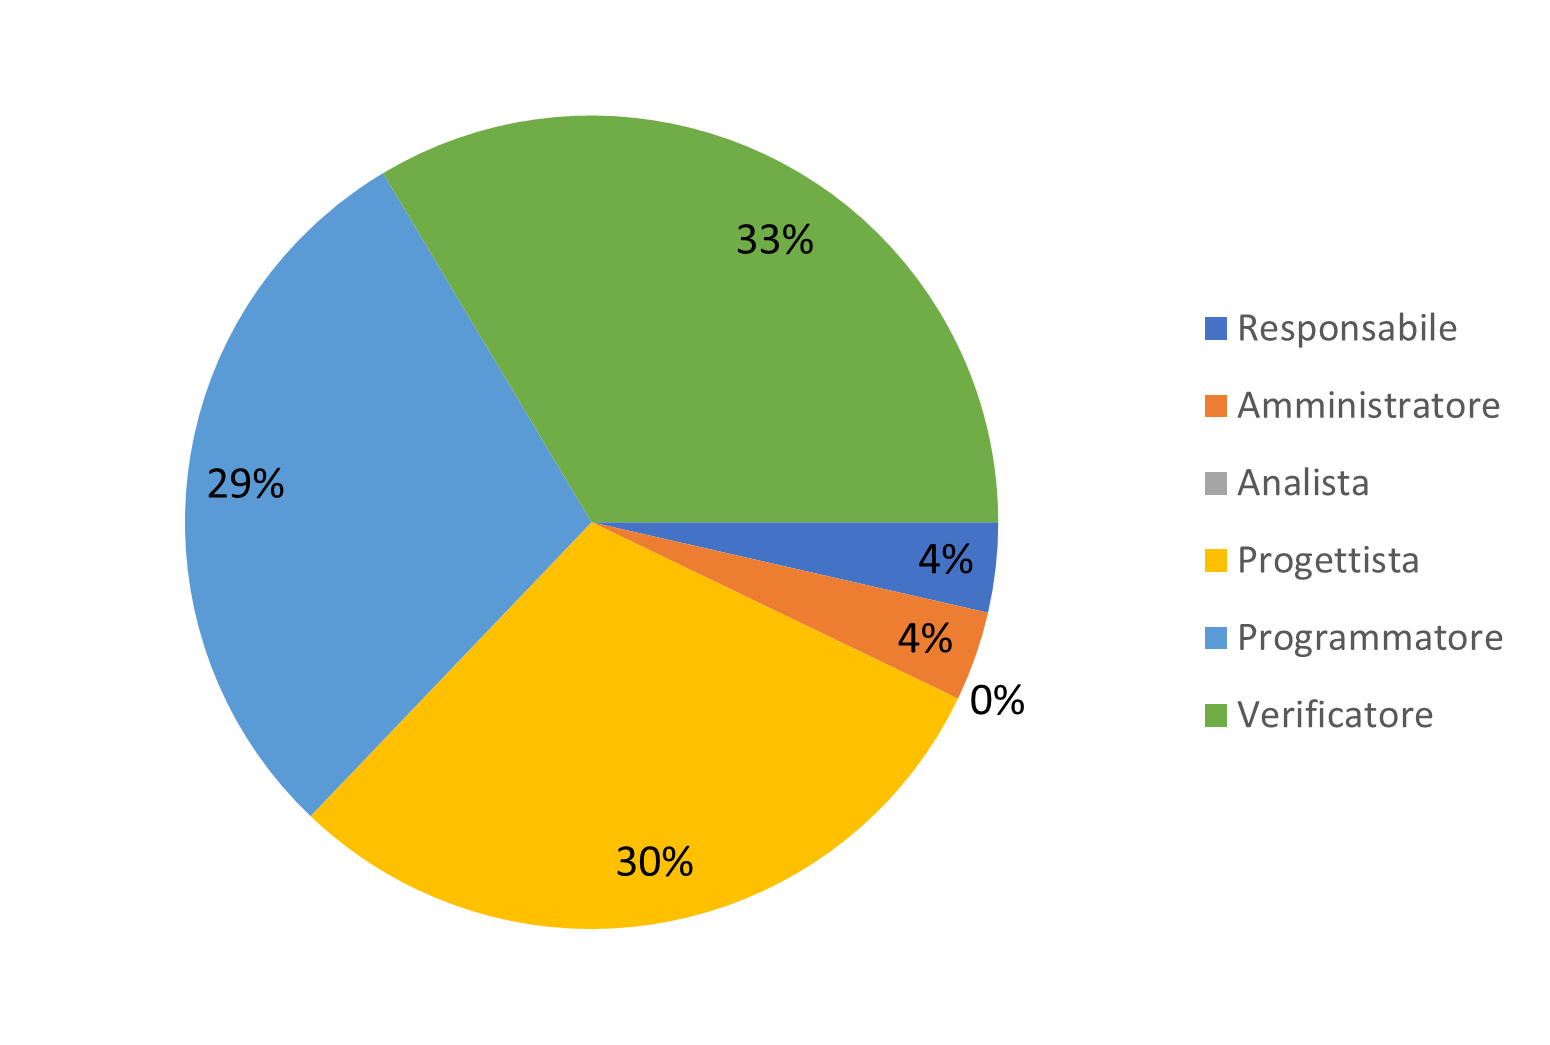
\includegraphics[width=0.8\linewidth]{res/images/preventivo/dettaglio_termineimp/1-2.png}
	\caption{Diagramma percentuale ore/ruolo nel VIII incremento}
	\label{fig:diagramma costi ruolo  VIII incremento}
\end{figure}

\subsubsection{IX incremento}
\paragraph{Prospetto orario}
Durante il IX incremento la distribuzione oraria sarà la seguente:

\rowcolors{1}{lightest-grayest}{blue!20}
\begin{longtable}{|l|c|c|c|c|c|c|c|}
	\hline
	\rowcolor{lighter-grayer}
	\textbf{Nome}     & \textbf{Re} & \textbf{Am} & \textbf{An} & \textbf{Pg} & \textbf{Pr} & \textbf{Ve} & \textbf{Totale} \\
	\hline
	\endfirsthead

	\hline
	Marco Canovese    & 0           & 0           & 0           & 2           & 2           & 4           & 8               \\
	\hline
	\hline
	Nicole Davanzo    & 0           & 2           & 0           & 2           & 0           & 4           & 8               \\
	\hline
	\hline
	Ivan Furlan       & 0           & 1           & 0           & 2           & 4           & 1           & 8               \\
	\hline
	\hline
	Gianmarco Guazzo  & 2           & 0           & 0           & 2           & 2           & 2           & 8               \\
	\hline
	\hline
	Stefano Lazzaroni & 0           & 0           & 0           & 2           & 2           & 4           & 8               \\
	\hline
	\hline
	Francesco Trolese & 0           & 0           & 0           & 2           & 3           & 3           & 8               \\
	\hline
	\hline
	Michele Veronesi  & 1           & 0           & 0           & 3           & 1           & 3           & 8               \\
	\hline
	\hline
	Totale            & 3           & 3          & 0          & 15           & 14           & 21          & 56              \\
	\hline
	\rowcolor{white}
	\caption{Tabella contenente il prospetto orario preventivato per il IX incremento}
\end{longtable}


La tabella può essere riassunta nel seguente istogramma:

\begin{figure}[H]
	\centering
	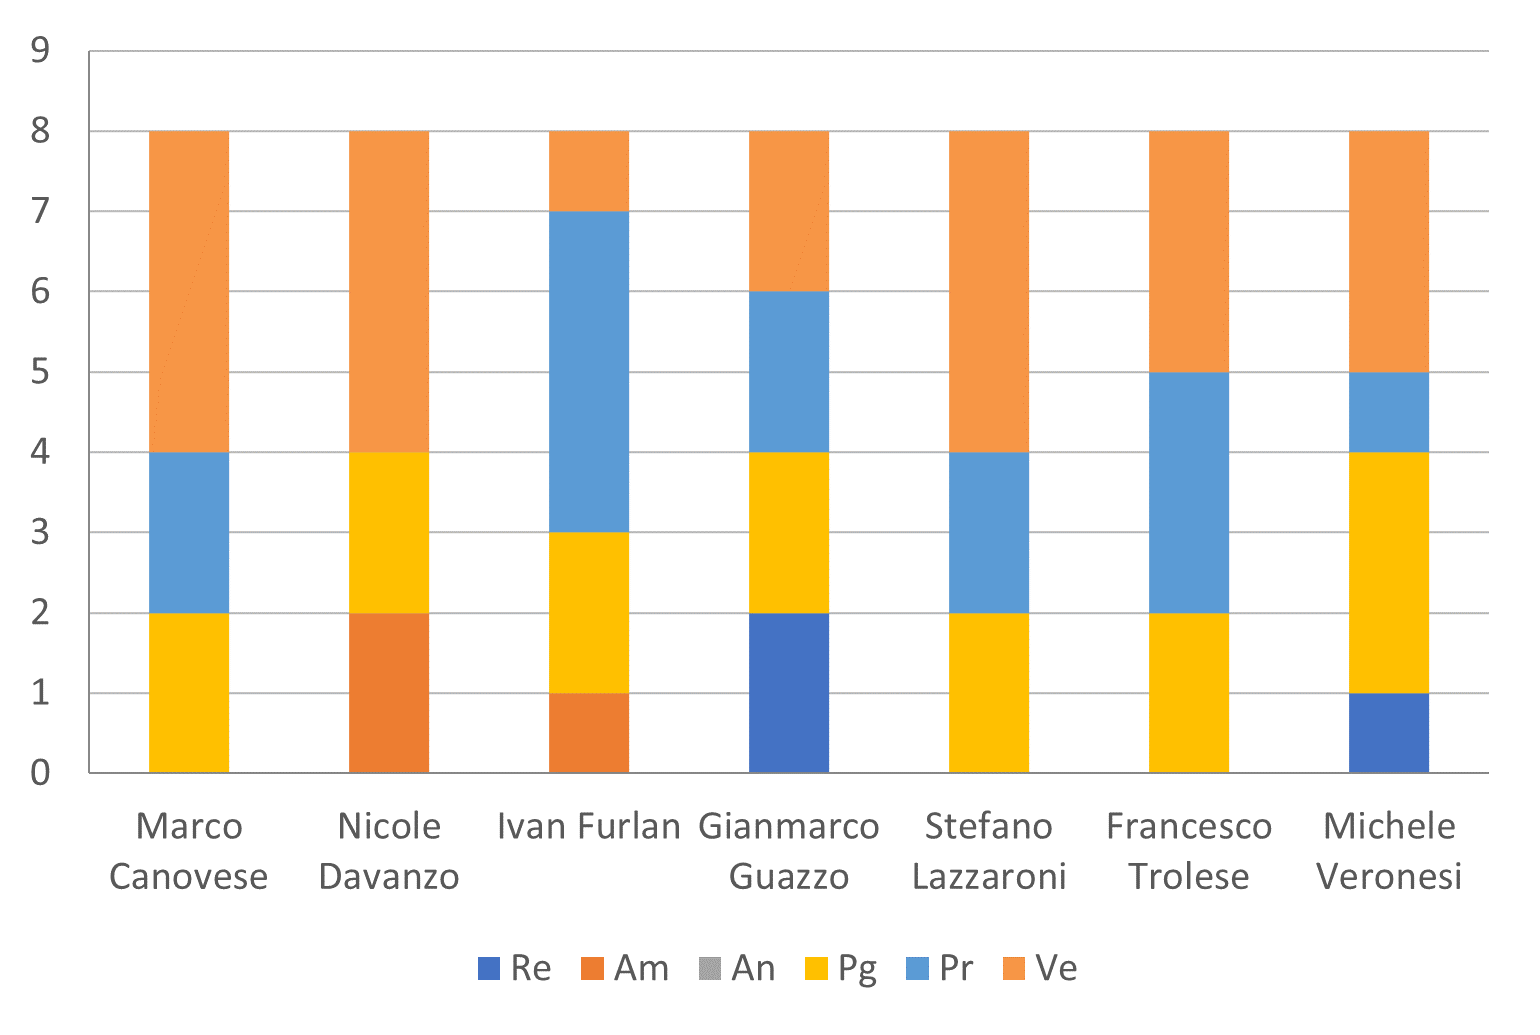
\includegraphics[width=0.8\linewidth]{res/images/preventivo/dettaglio_termineimp/2-1.png}
	\caption{Diagramma ore/ruolo componenti nel IX incremento}
	\label{fig:diagramma suddivisione ruoli IX incremento}
\end{figure}

\paragraph{Prospetto economico}
In base al prospetto orario, quello economico sarà il seguente:

\rowcolors{1}{lightest-grayest}{blue!20}
\begin{longtable}{|l|c|c|c|c|c|c|c|}
	\hline
	\rowcolor{lighter-grayer}
	\textbf{Ruolo}  & \textbf{Ore} & \textbf{Costo in €} \\
	\hline
	\endfirsthead

	\hline
	Responsabile    & 3            & 90,00              \\
	\hline
	\hline
	Amministratore  & 3           & 60,00              \\
	\hline
	\hline
	Analista        & 0           & 00,00              \\
	\hline
	\hline
	Progettista     & 15            & 330,00                   \\
	\hline
	\hline
	Programmatore   & 14            & 210,00                   \\
	\hline
	\hline
	Verificatore    & 21           & 315,00              \\
	\hline
	\hline
	\textbf{Totale} & 56           & 1.005,00            \\
	\hline
	\rowcolor{white}
	\caption{Tabella contenente il prospetto economico in riferimento al prospetto orario}
\end{longtable}
\pagebreak

La tabella può essere riassunta nel seguente areogramma:
\begin{figure}[H]
	\centering
	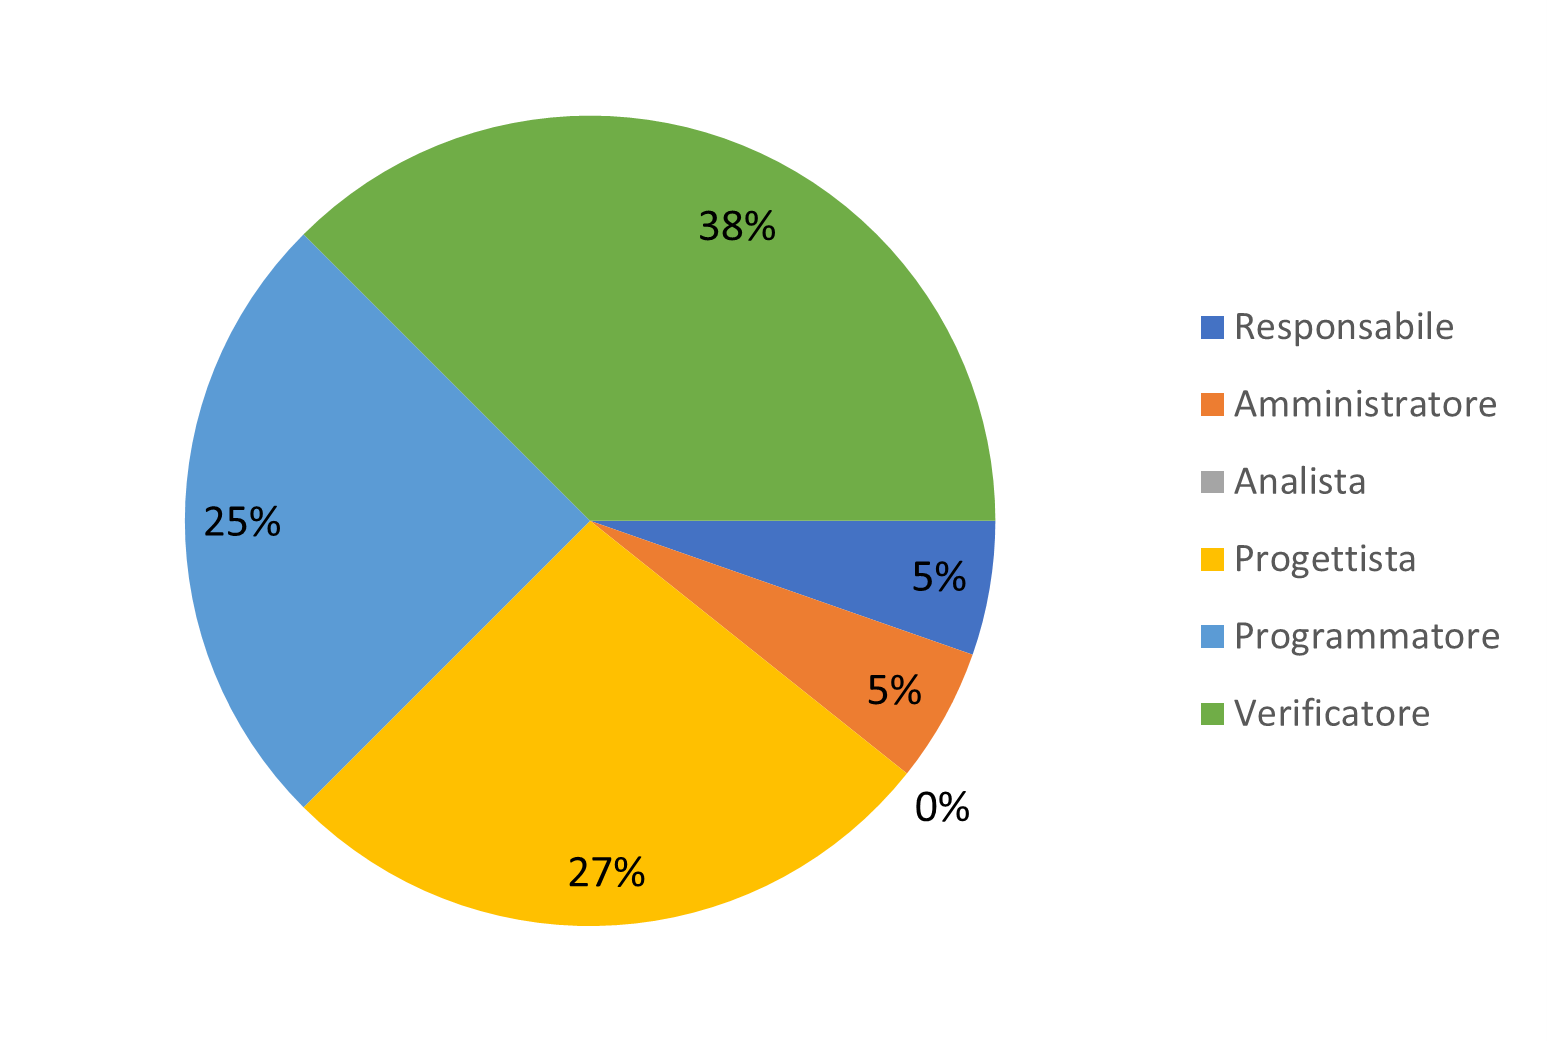
\includegraphics[width=0.8\linewidth]{res/images/preventivo/dettaglio_termineimp/2-2.png}
	\caption{Diagramma percentuale ore/ruolo nel IX incremento}
	\label{fig:diagramma costi ruolo IX incremento}
\end{figure}
\subsubsection{Fase complessiva}

\paragraph{Prospetto orario}
Durante la fase di termine dell'implementazione e raffinamento generale la distribuzione oraria sarà la seguente:

\rowcolors{1}{lightest-grayest}{blue!20}
\begin{longtable}{|l|c|c|c|c|c|c|c|}
	\hline
	\rowcolor{lighter-grayer}
	\textbf{Nome}     & \textbf{Re} & \textbf{Am} & \textbf{An} & \textbf{Pg} & \textbf{Pr} & \textbf{Ve} & \textbf{Totale} \\
	\hline
	\endfirsthead

	\hline
	Marco Canovese    & 0           & 0           & 0           & 5           & 7           & 12          & 24              \\
	\hline
	\hline
	Nicole Davanzo    & 1           & 5           & 0           & 5           & 3           & 10          & 24              \\
	\hline
	\hline
	Ivan Furlan       & 0           & 3           & 0           & 5           & 10          & 6           & 24              \\
	\hline
	\hline
	Gianmarco Guazzo  & 4           & 0           & 0           & 3           & 8           & 9           & 24              \\
	\hline
	\hline
	Stefano Lazzaroni & 0           & 0           & 0           & 6           & 8           & 10          & 24              \\
	\hline
	\hline
	Francesco Trolese & 0           & 0           & 0           & 4           & 10          & 10          & 24              \\
	\hline
	\hline
	Michele Veronesi  & 3           & 0           & 0           & 8           & 2           & 11          & 24              \\
	\hline
	\hline
	Totale            & 8           & 8           & 0           & 36          & 48          & 68          & 168             \\
	\hline
	\rowcolor{white}
	\caption{Tabella contenente il prospetto orario preventivato per la fase di Termine dell'implementazione e raffinamento generale}
\end{longtable}


La tabella può essere riassunta nel seguente istogramma:

\begin{figure}[H]
	\centering
	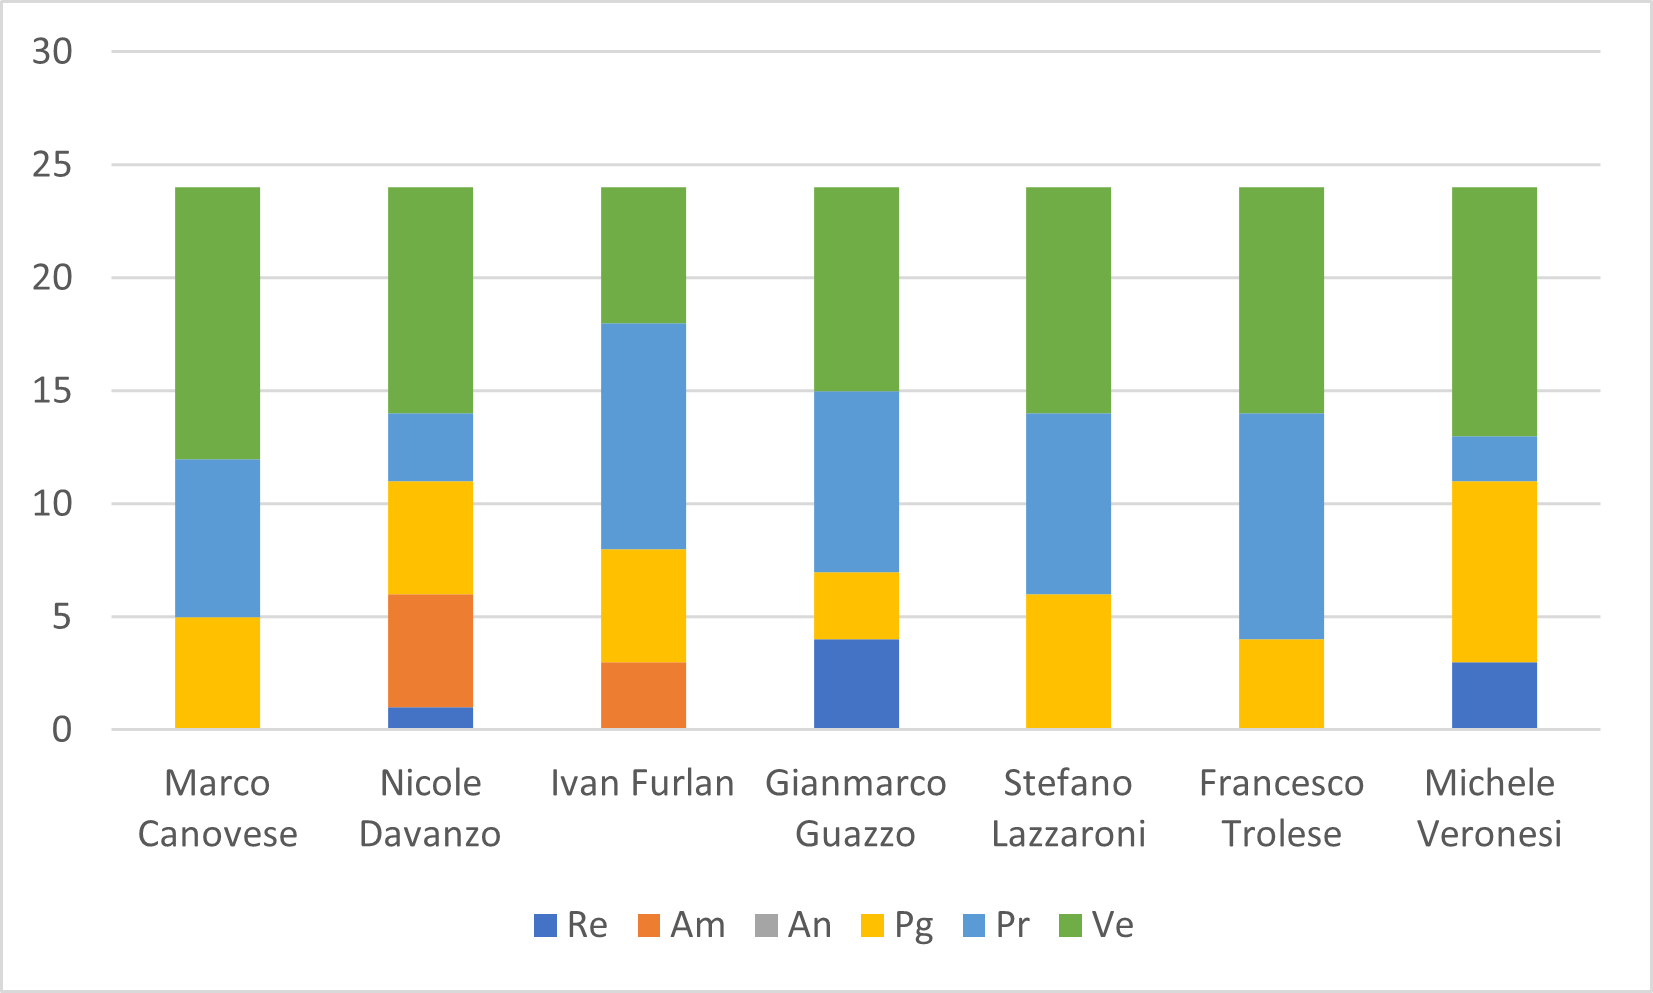
\includegraphics[width=0.8\linewidth]{res/images/preventivo/6-1.png}
	\caption{Diagramma ore/ruolo componenti nella fase di Termine dell'implementazione e raffinamento generale}
	\label{fig:diagramma suddivisione ruoli fase Termine dell'implementazione e raffinamento generale}
\end{figure}

\paragraph{Prospetto economico}
In base al prospetto orario, quello economico sarà il seguente:

\rowcolors{1}{lightest-grayest}{blue!20}
\begin{longtable}{|l|c|c|c|c|c|c|c|}
	\hline
	\rowcolor{lighter-grayer}
	\textbf{Ruolo}  & \textbf{Ore} & \textbf{Costo in €} \\
	\hline
	\endfirsthead

	\hline
	Responsabile    & 8            & 240,00              \\
	\hline
	\hline
	Amministratore  & 8            & 160,00              \\
	\hline
	\hline
	Analista        & -            & -                   \\
	\hline
	\hline
	Progettista     & 36           & 792,00              \\
	\hline
	\hline
	Programmatore   & 48           & 720,00              \\
	\hline
	\hline
	Verificatore    & 68           & 1.020,00            \\
	\hline
	\hline
	\textbf{Totale} & 168          & 2.932,00            \\
	\hline
	\rowcolor{white}
	\caption{Tabella contenente il prospetto economico in riferimento al prospetto orario}
\end{longtable}
\pagebreak

La tabella può essere riassunta nel seguente areogramma:
\begin{figure}[H]
	\centering
	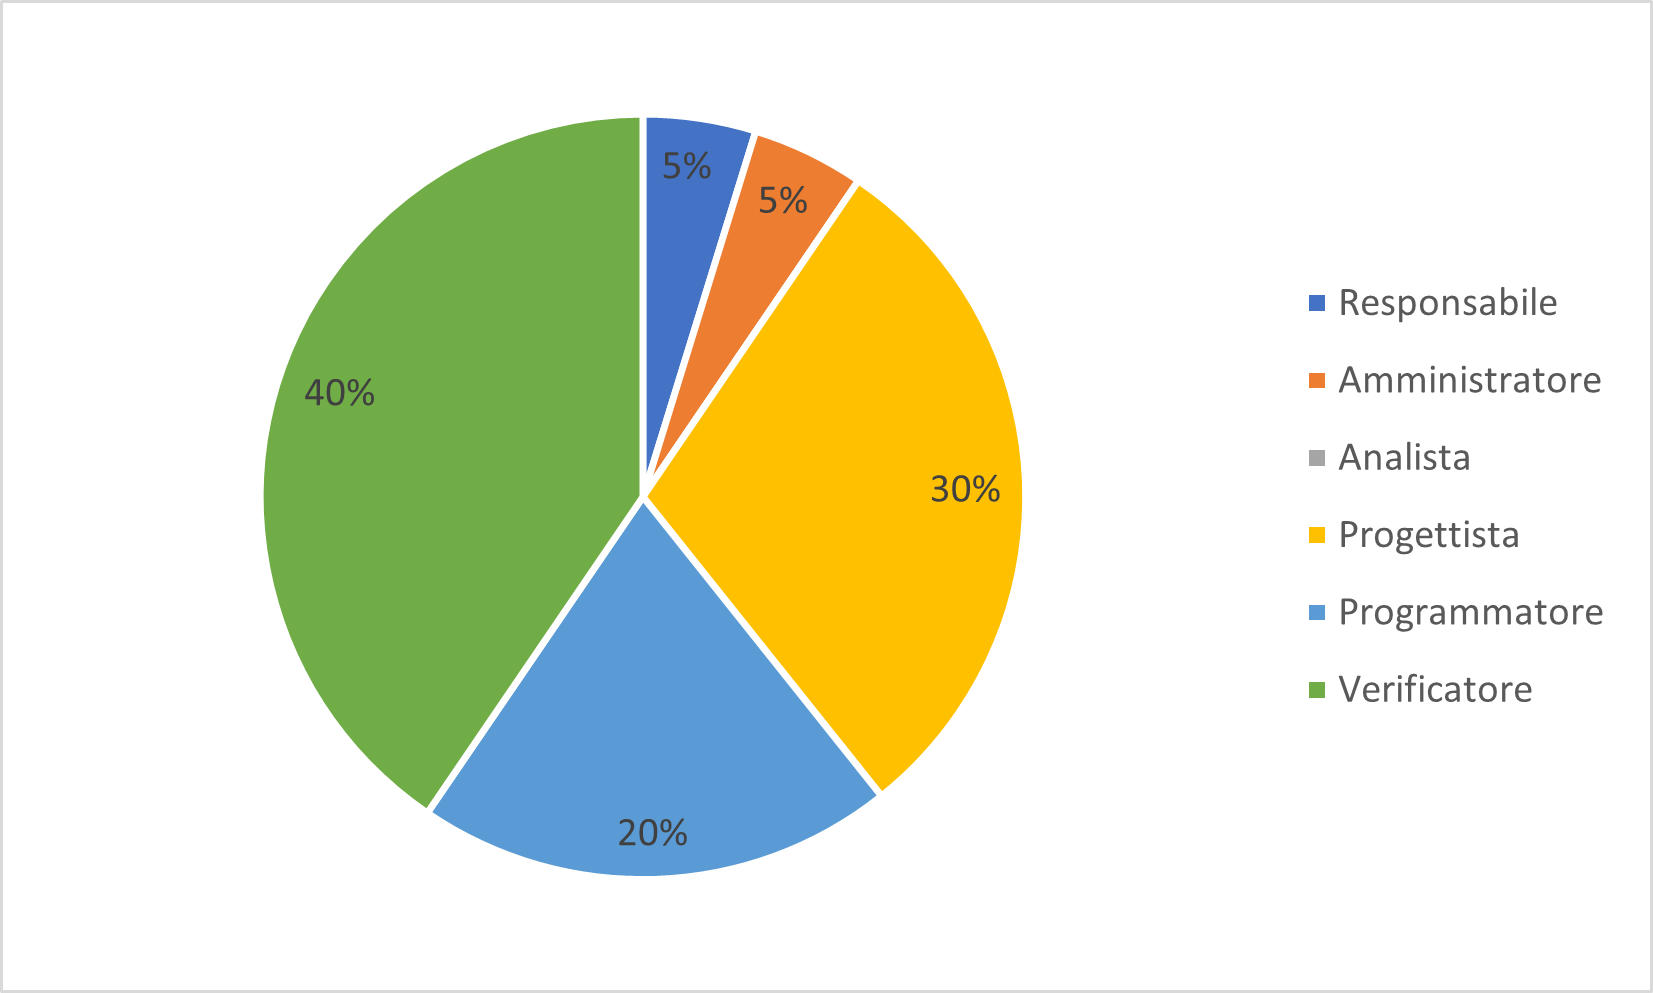
\includegraphics[width=0.8\linewidth]{res/images/preventivo/6-2.png}
	\caption{Diagramma percentuale ore/ruolo nella fase di Termine dell'implementazione e raffinamento generale}
	\label{fig:diagramma costi ruolo fase Termine dell'implementazione e raffinamento generale}
\end{figure}

\subsection{Validazione e collaudo}
\subsubsection{Prospetto orario}
Durante la fase di validazione e collaudo la distribuzione oraria sarà la seguente:

\rowcolors{1}{lightest-grayest}{blue!20}
\begin{longtable}{|l|c|c|c|c|c|c|c|}
	\hline
	\rowcolor{lighter-grayer}
	\textbf{Nome}     & \textbf{Re} & \textbf{Am} & \textbf{An} & \textbf{Pg} & \textbf{Pr} & \textbf{Ve} & \textbf{Totale} \\
	\hline
	\endfirsthead

	\hline
	Marco Canovese    & 5           & 2           & 0           & 0           & 2           & 5           & 14              \\
	\hline
	\hline
	Nicole Davanzo    & 3           & 0           & 0           & 3           & 4           & 4           & 14              \\
	\hline
	\hline
	Ivan Furlan       & 0           & 4           & 4           & 3           & 0           & 3           & 14              \\
	\hline
	\hline
	Gianmarco Guazzo  & 3           & 3           & 0           & 2           & 0           & 6           & 14              \\
	\hline
	\hline
	Stefano Lazzaroni & 0           & 4           & 2           & 2           & 6           & 0           & 14              \\
	\hline
	\hline
	Francesco Trolese & 0           & 3           & 5           & 0           & 3           & 3           & 14              \\
	\hline
	\hline
	Michele Veronesi  & 3           & 0           & 4           & 1           & 2           & 4           & 14              \\
	\hline
	\hline
	Totale            & 14          & 16          & 15          & 11          & 17          & 25          & 98              \\
	\hline
	\rowcolor{white}
	\caption{Tabella contenente il prospetto orario preventivato per la fase di validazione e collaudo.}
\end{longtable}


La tabella può essere riassunta nel seguente istogramma:

\begin{figure}[H]
	\centering
	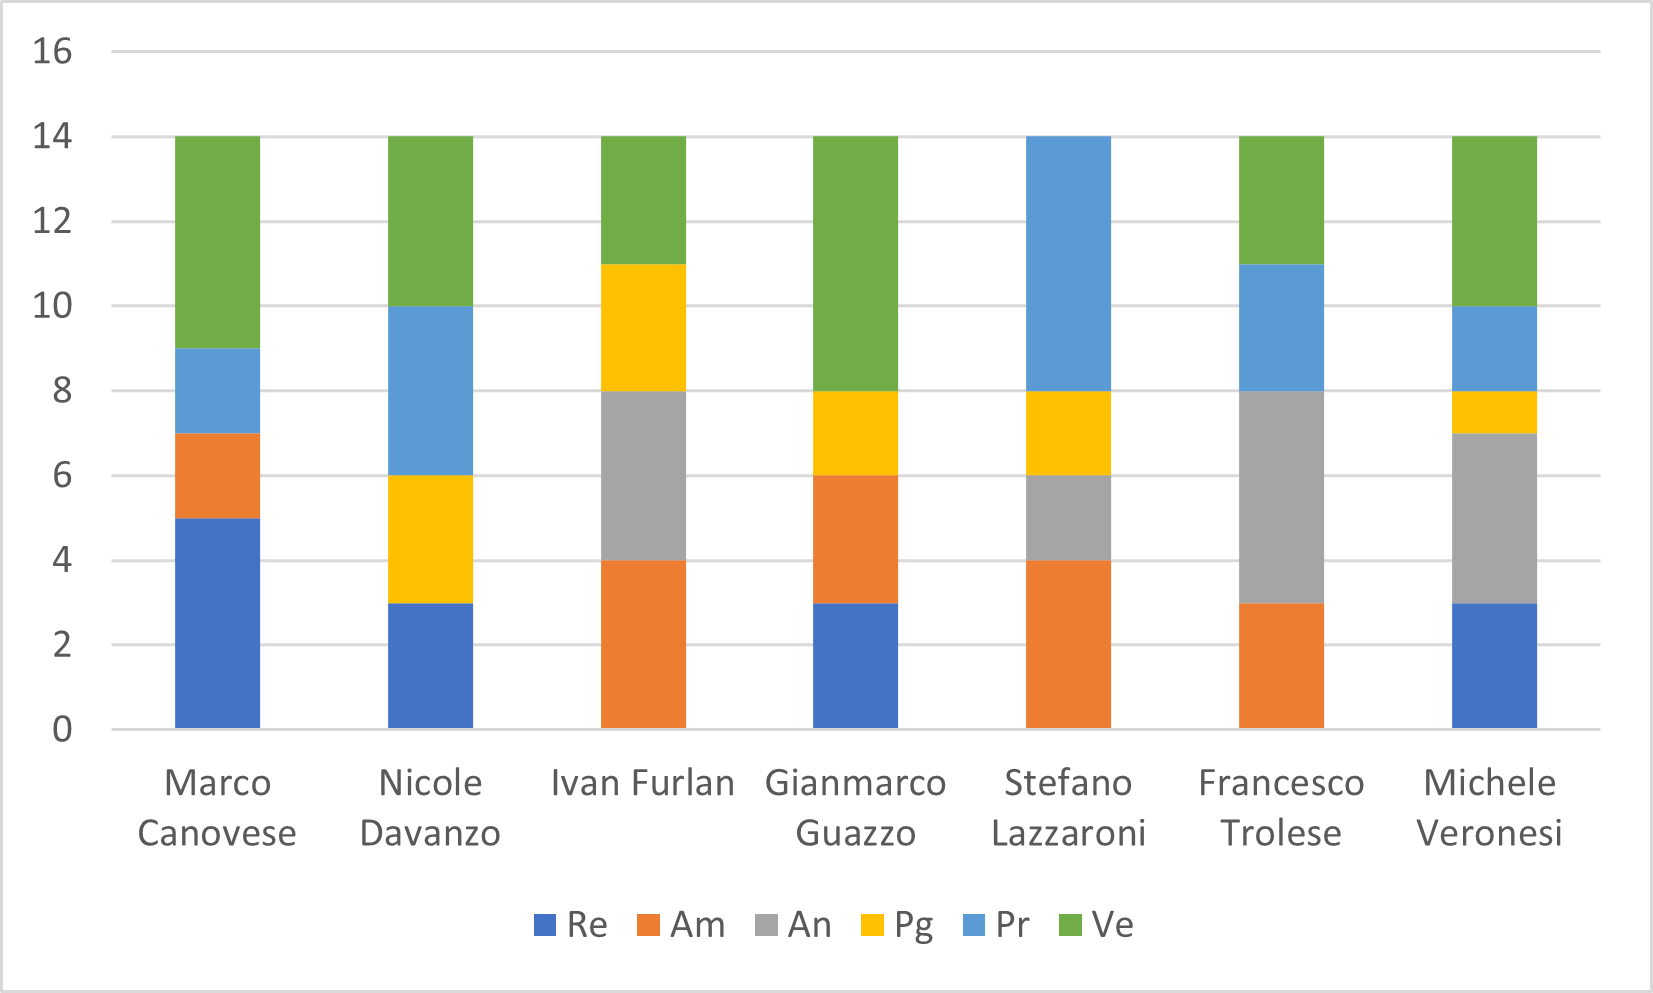
\includegraphics[width=0.8\linewidth]{res/images/preventivo/7-1.png}
	\caption{Diagramma ore/ruolo componenti nella fase di Validazione e collaudo.}
	\label{fig:diagramma suddivisione ruoli fase Validazione e collaudo.}
\end{figure}

\subsubsection{Prospetto economico}
In base al prospetto orario, quello economico sarà il seguente:

\rowcolors{1}{lightest-grayest}{blue!20}
\begin{longtable}{|l|c|c|c|c|c|c|c|}
	\hline
	\rowcolor{lighter-grayer}
	\textbf{Ruolo}  & \textbf{Ore} & \textbf{Costo in €} \\
	\hline
	\endfirsthead

	\hline
	Responsabile    & 14           & 420,00              \\
	\hline
	\hline
	Amministratore  & 16           & 320,00              \\
	\hline
	\hline
	Analista        & 15           & 375,00              \\
	\hline
	\hline
	Progettista     & 11           & 242,00              \\
	\hline
	\hline
	Programmatore   & 17           & 255,00              \\
	\hline
	\hline
	Verificatore    & 25           & 375,00              \\
	\hline
	\hline
	\textbf{Totale} & 98           & 1.987,00            \\
	\hline
	\rowcolor{white}
	\caption{Tabella contenente il prospetto economico in riferimento al prospetto orario}
\end{longtable}
\pagebreak

La tabella può essere riassunta nel seguente areogramma:
\begin{figure}[H]
	\centering
	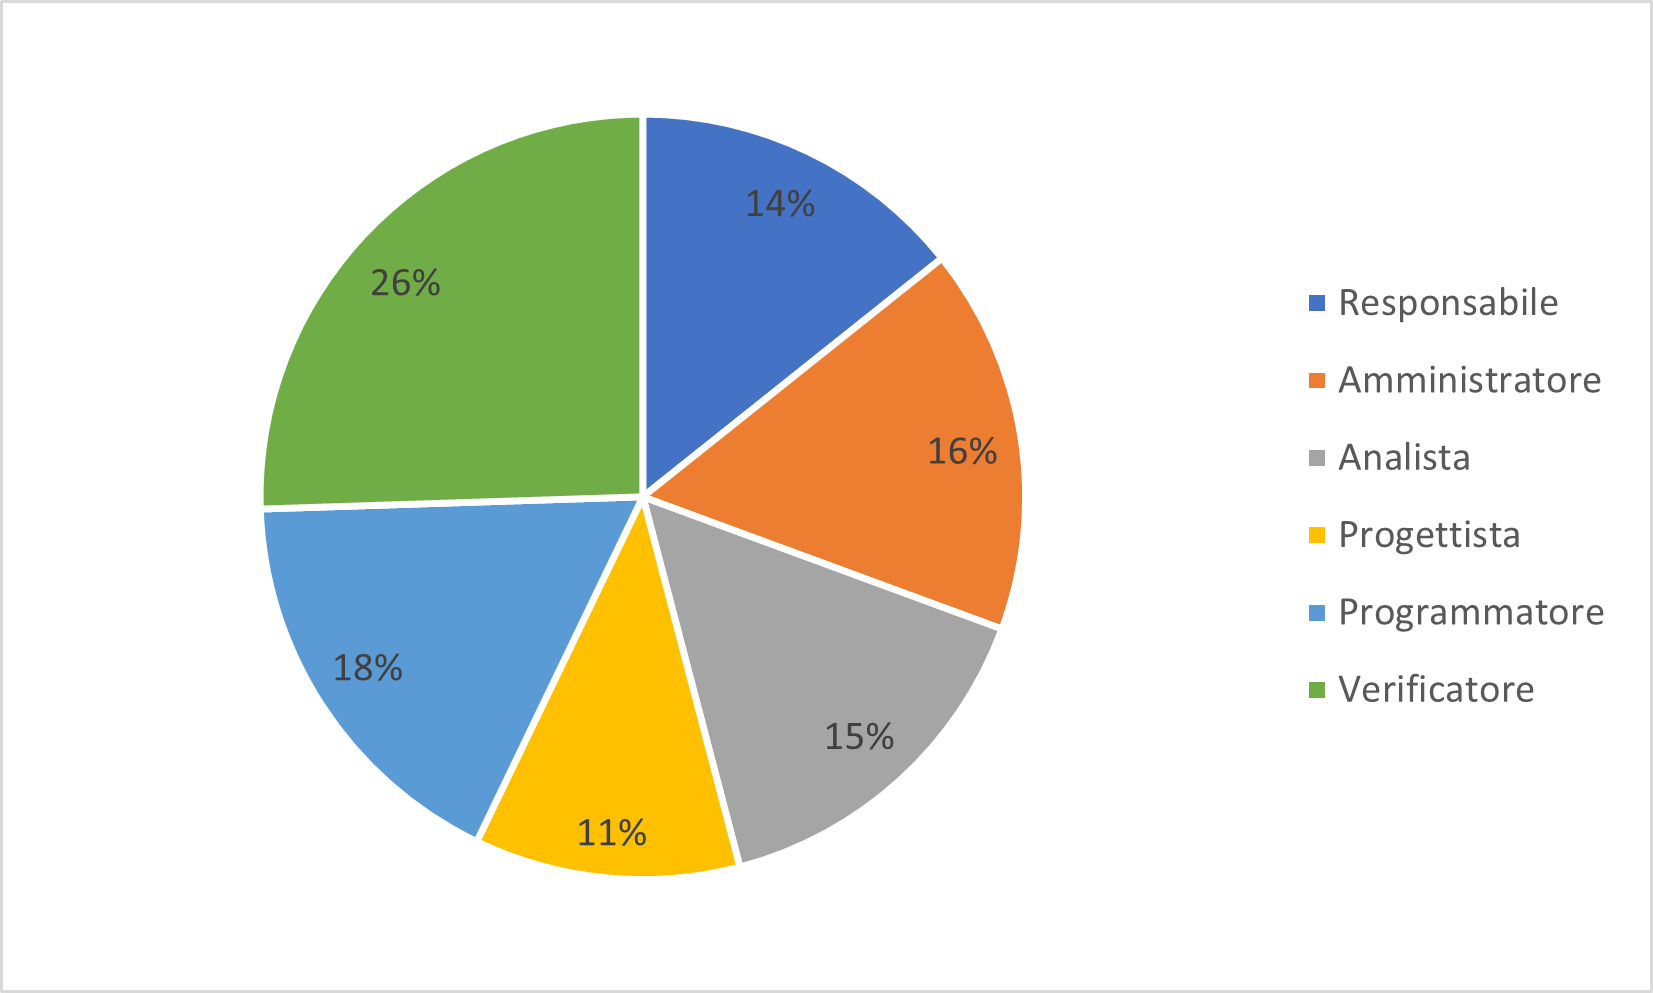
\includegraphics[width=0.8\linewidth]{res/images/preventivo/7-2.png}
	\caption{Diagramma percentuale ore/ruolo nella fase di Validazione e collaudo.}
	\label{fig:diagramma costi ruolo fase Validazione e collaudo.}
\end{figure}

\subsection{Riepilogo ore totali}
\subsubsection{Totale orario complessivo}
\paragraph{Prospetto orario complessivo}
Riepilogo della distribuzione oraria di tutte le fasi:

\rowcolors{1}{lightest-grayest}{blue!20}
\begin{longtable}{|l|c|c|c|c|c|c|c|}
	\hline
	\rowcolor{lighter-grayer}
	\textbf{Nome}     & \textbf{Re} & \textbf{Am} & \textbf{An} & \textbf{Pg} & \textbf{Pr} & \textbf{Ve} & \textbf{Totale} \\
	\hline
	\endfirsthead

	\hline
	Marco Canovese    & 13          & 17          & 16          & 20          & 28          & 41          & 135             \\
	\hline
	\hline
	Nicole Davanzo    & 12          & 16          & 15          & 25          & 24          & 43          & 135             \\
	\hline
	\hline
	Ivan Furlan       & 11          & 17          & 23          & 18          & 25          & 41          & 135             \\
	\hline
	\hline
	Gianmarco Guazzo  & 14          & 17          & 17          & 28          & 22          & 37          & 135             \\
	\hline
	\hline
	Stefano Lazzaroni & 10          & 13          & 17          & 34          & 24          & 37          & 135             \\
	\hline
	\hline
	Francesco Trolese & 11          & 14          & 22          & 19          & 26          & 43          & 135             \\
	\hline
	\hline
	Michele Veronesi  & 13          & 13          & 23          & 23          & 23          & 40          & 135             \\
	\hline
	\hline
	Totale            & 84          & 107         & 133         & 167         & 172         & 282         & 945             \\
	\hline
	\rowcolor{white}
	\caption{Tabella contenente il prospetto orario preventivato tenendo conto di tutte le fasi}
\end{longtable}


La tabella può essere riassunta nel seguente istogramma:

\begin{figure}[H]
	\centering
	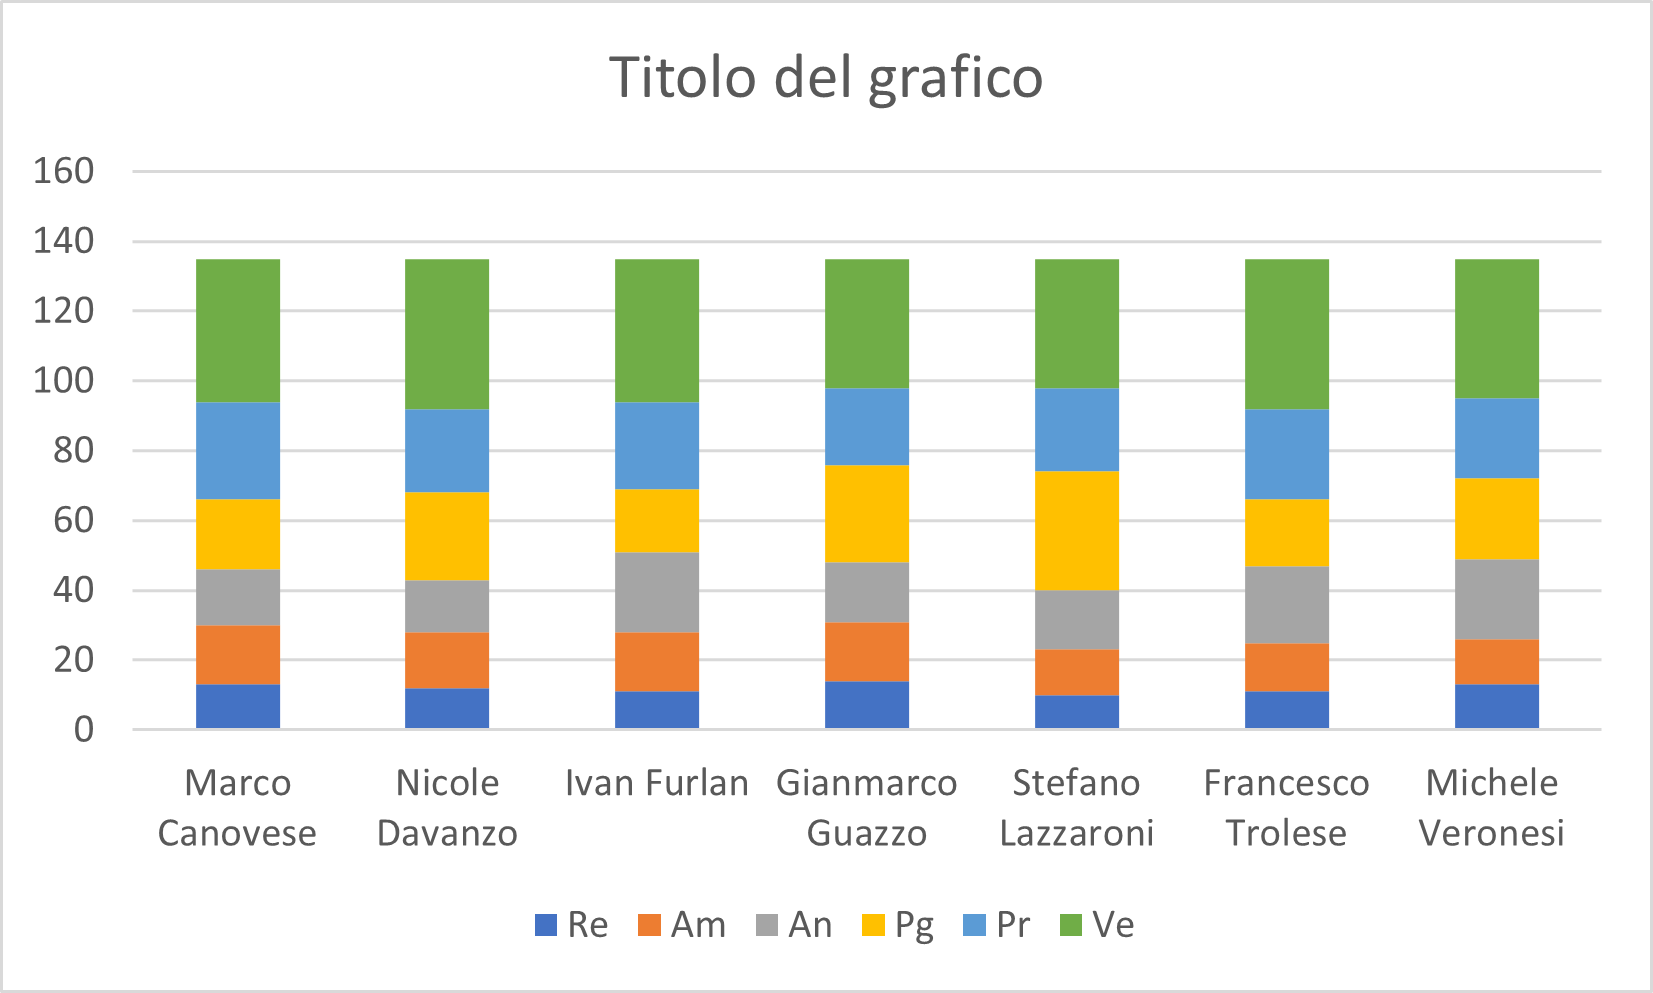
\includegraphics[width=0.8\linewidth]{res/images/preventivo/tot1.png}
	\caption{Diagramma ore/ruolo componenti riepilogativa di tutte le fasi}
	\label{fig:diagramma suddivisione ruoli riepilogativa di tutte le fasi}
\end{figure}

\paragraph{Prospetto economico complessivo}
In base al prospetto orario, quello economico sarà il seguente:

\rowcolors{1}{lightest-grayest}{blue!20}
\begin{longtable}{|l|c|c|c|c|c|c|c|}
	\hline
	\rowcolor{lighter-grayer}
	\textbf{Ruolo}  & \textbf{Ore} & \textbf{Costo in €} \\
	\hline
	\endfirsthead

	\hline
	Responsabile    & 84           & 2.520,00            \\
	\hline
	\hline
	Amministratore  & 107          & 2.140,00            \\
	\hline
	\hline
	Analista        & 133          & 3.325,00            \\
	\hline
	\hline
	Progettista     & 167          & 3.674,00            \\
	\hline
	\hline
	Programmatore   & 172          & 2.580,00            \\
	\hline
	\hline
	Verificatore    & 282          & 4.230,00            \\
	\hline
	\hline
	\textbf{Totale} & 945          & 18.469,00           \\
	\hline
	\rowcolor{white}
	\caption{Tabella contenente il prospetto economico in riferimento al prospetto orario}
\end{longtable}
\pagebreak

La tabella può essere riassunta nel seguente areogramma:
\begin{figure}[H]
	\centering
	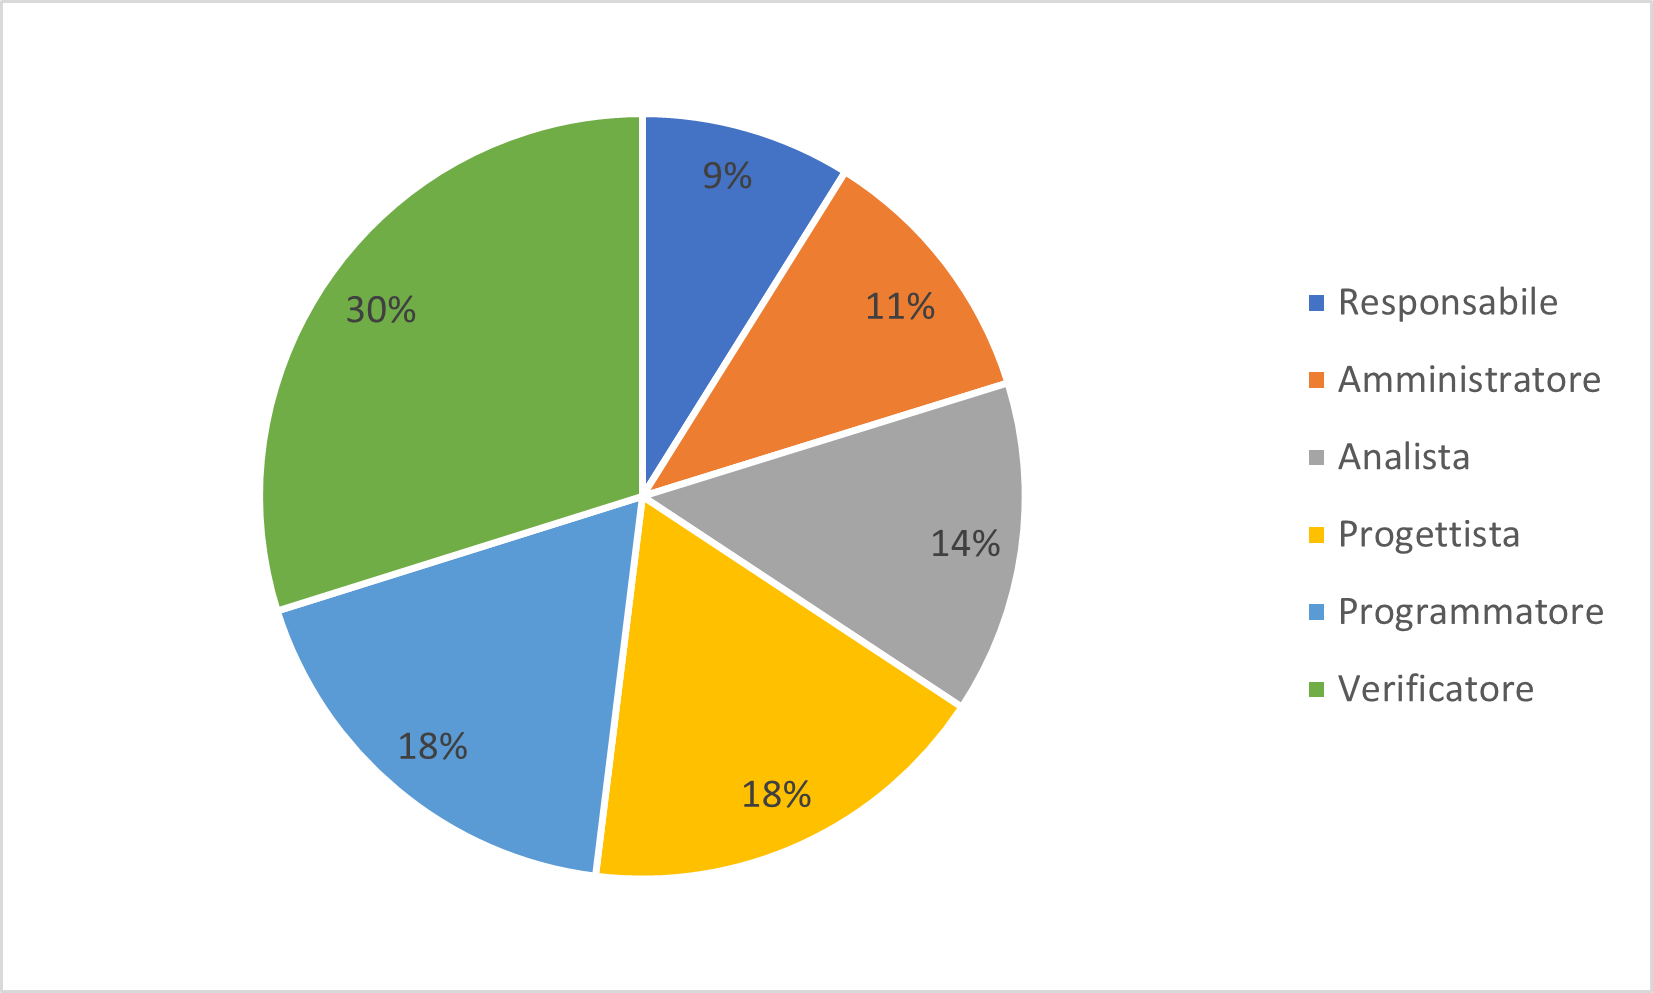
\includegraphics[width=0.8\linewidth]{res/images/preventivo/tot2.png}
	\caption{Diagramma percentuale ore/ruolo riepilogativa di tutte le fasi}
	\label{fig:diagramma costi ruolo riepilogativa di tutte le fasi}
\end{figure}

\subsubsection{Totale orario rendicontato}
\paragraph{Prospetto orario rendicontato}
Riepilogo della distribuzione oraria delle fasi rendicontate, escludendo quindi le fasi di
analisi e consolidamento dei requisiti:

\rowcolors{1}{lightest-grayest}{blue!20}
\begin{longtable}{|l|c|c|c|c|c|c|c|}
	\hline
	\rowcolor{lighter-grayer}
	\textbf{Nome}     & \textbf{Re} & \textbf{Am} & \textbf{An} & \textbf{Pg} & \textbf{Pr} & \textbf{Ve} & \textbf{Totale} \\
	\hline
	\endfirsthead

	\hline
	Marco Canovese    & 11          & 7           & 5           & 20          & 28          & 29          & 100             \\
	\hline
	\hline
	Nicole Davanzo    & 4           & 15          & 0           & 25          & 24          & 32          & 100             \\
	\hline
	\hline
	Ivan Furlan       & 11          & 10          & 9           & 18          & 25          & 27          & 100             \\
	\hline
	\hline
	Gianmarco Guazzo  & 10          & 11          & 3           & 28          & 22          & 26          & 100             \\
	\hline
	\hline
	Stefano Lazzaroni & 2           & 8           & 5           & 34          & 24          & 27          & 100             \\
	\hline
	\hline
	Francesco Trolese & 4           & 9           & 14          & 19          & 26          & 28          & 100             \\
	\hline
	\hline
	Michele Veronesi  & 11          & 7           & 14          & 23          & 23          & 22          & 100             \\
	\hline
	\hline
	Totale            & 53          & 67          & 50          & 167         & 172         & 191         & 700             \\
	\hline
	\rowcolor{white}
	\caption{Tabella contenente il prospetto orario preventivato tenendo conto delle fasi rendicontate}
\end{longtable}


La tabella può essere riassunta nel seguente istogramma:

\begin{figure}[H]
	\centering
	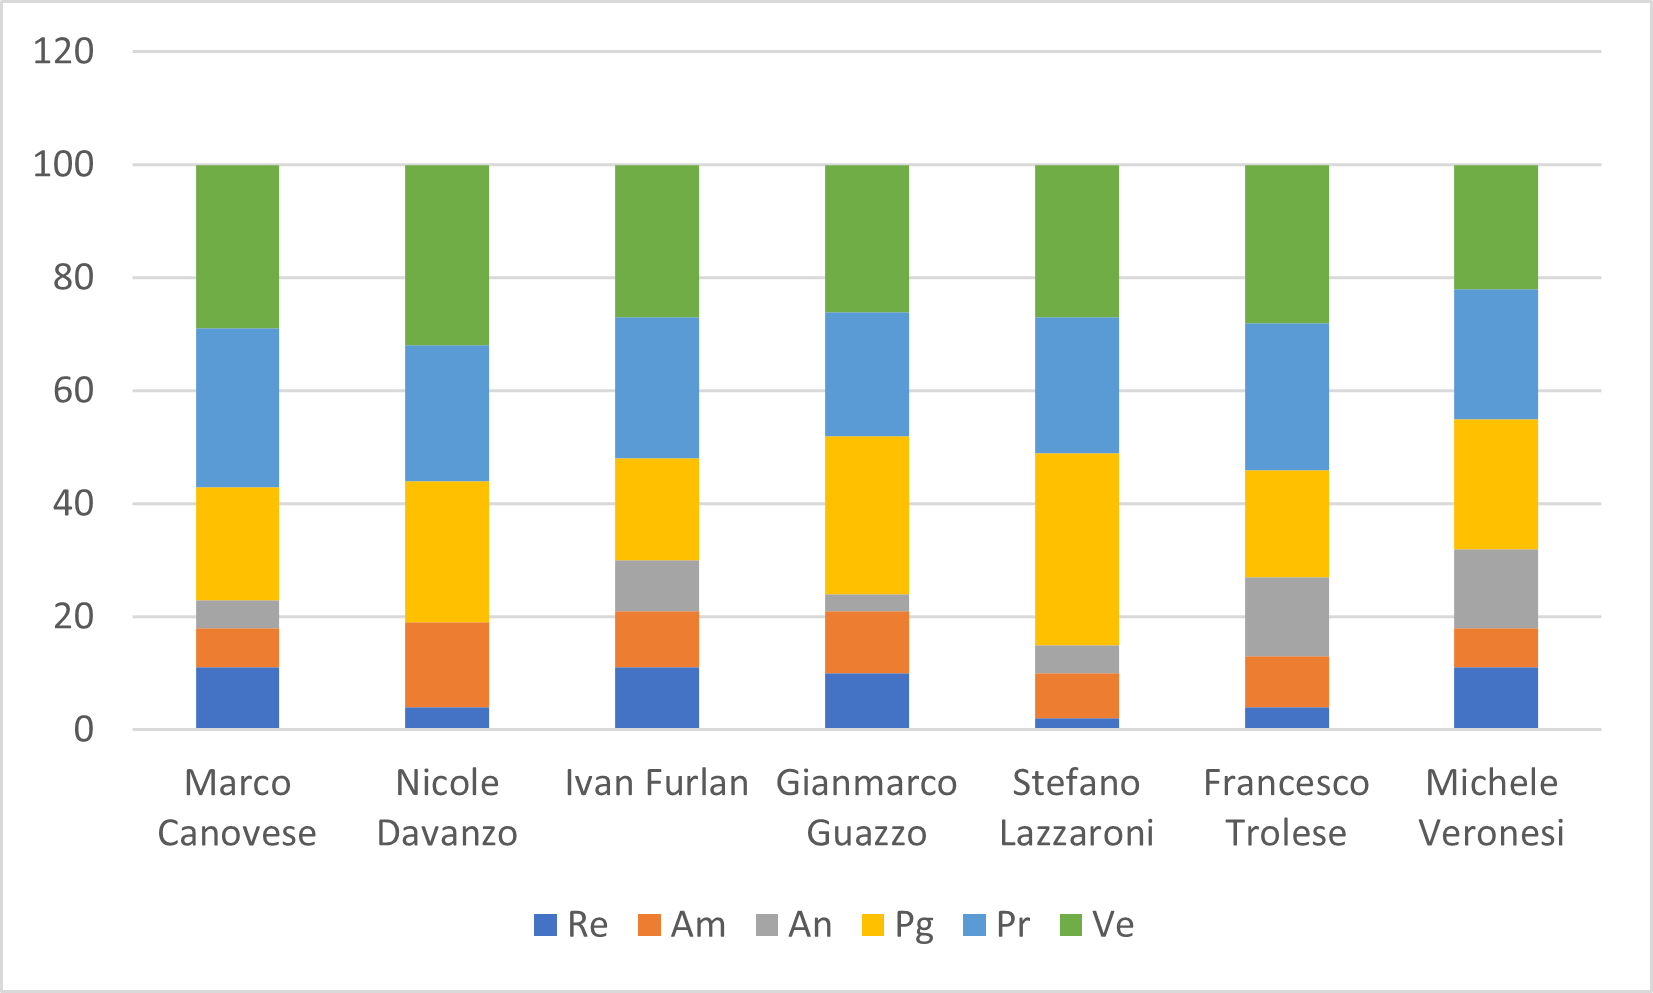
\includegraphics[width=0.8\linewidth]{res/images/preventivo/totrend1.png}
	\caption{Diagramma ore/ruolo componenti riepilogativa delle fasi rendicontate}
	\label{fig:diagramma suddivisione ruoli riepilogativa delle fasi rendicontate}
\end{figure}

\paragraph{Prospetto economico rendicontato}
In base al prospetto orario, quello economico sarà il seguente:

\rowcolors{1}{lightest-grayest}{blue!20}
\begin{longtable}{|l|c|c|c|c|c|c|c|}
	\hline
	\rowcolor{lighter-grayer}
	\textbf{Ruolo}  & \textbf{Ore} & \textbf{Costo in €} \\
	\hline
	\endfirsthead

	\hline
	Responsabile    & 53           & 1.590,00            \\
	\hline
	\hline
	Amministratore  & 67           & 1.340,00            \\
	\hline
	\hline
	Analista        & 50           & 1.250,00            \\
	\hline
	\hline
	Progettista     & 167          & 3.674,00            \\
	\hline
	\hline
	Programmatore   & 172          & 2.580,00            \\
	\hline
	\hline
	Verificatore    & 191          & 2.865,00            \\
	\hline
	\hline
	\textbf{Totale} & 700          & 13.299,00           \\
	\hline
	\rowcolor{white}
	\caption{Tabella contenente il prospetto economico in riferimento al prospetto orario}
\end{longtable}
\pagebreak

La tabella può essere riassunta nel seguente areogramma:
\begin{figure}[H]
	\centering
	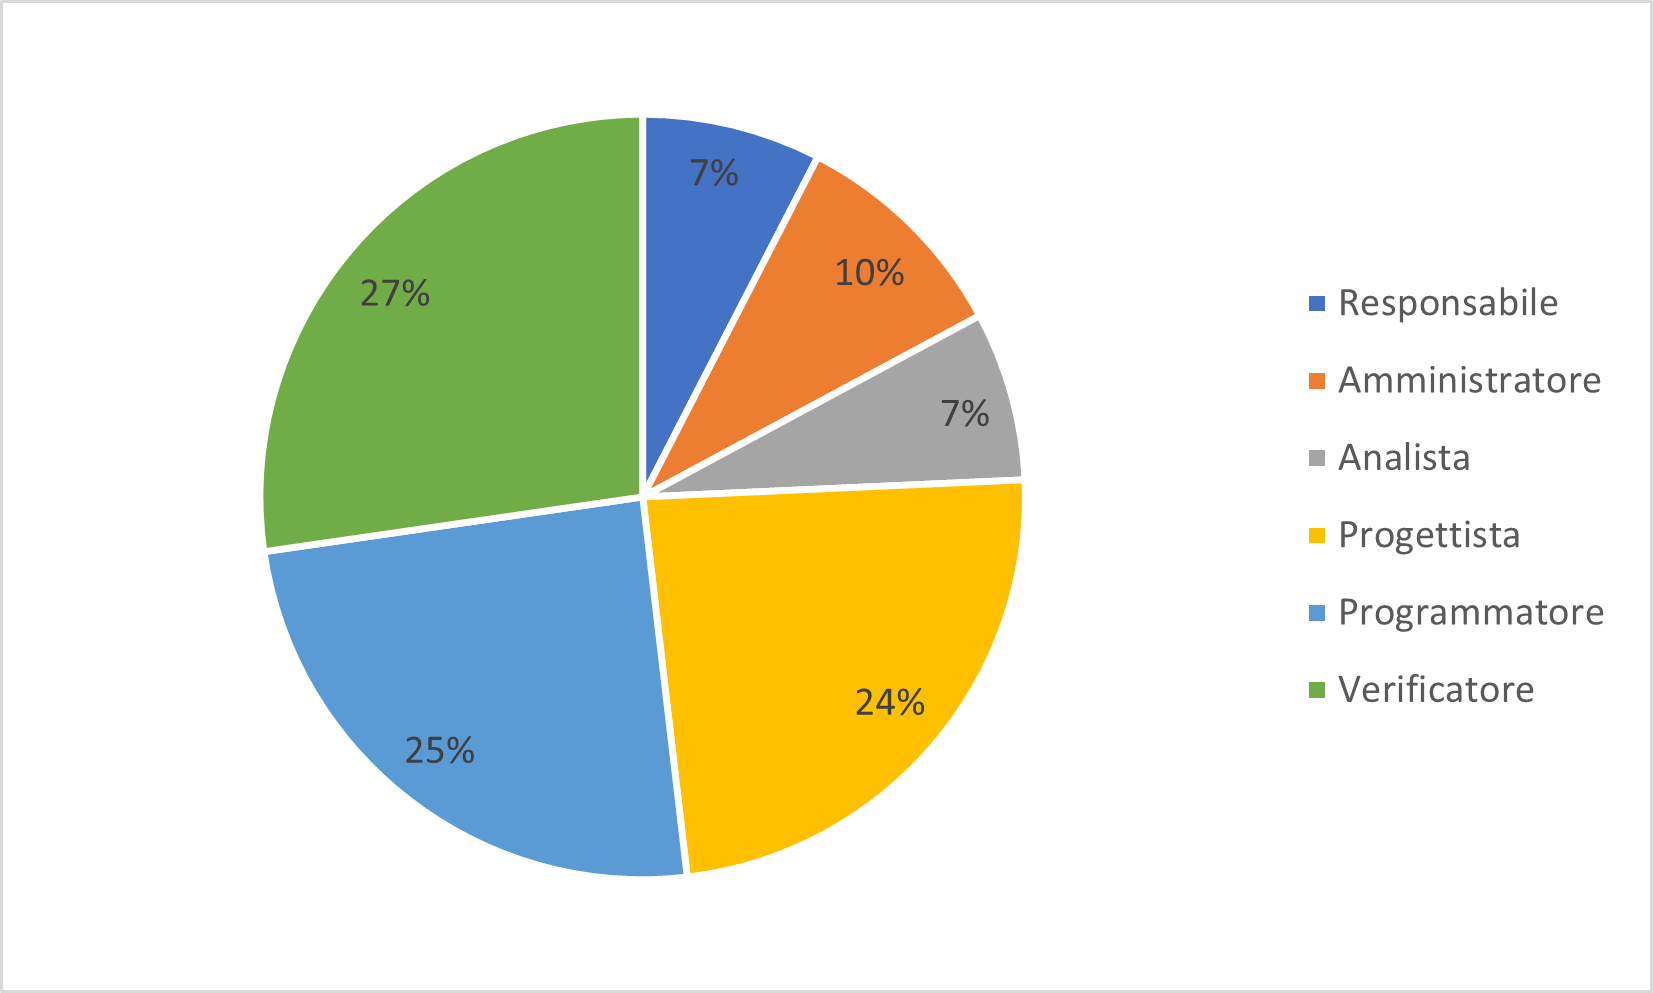
\includegraphics[width=0.8\linewidth]{res/images/preventivo/totrend2.png}
	\caption{Diagramma percentuale ore/ruolo riepilogativa delle fasi rendicontate}
	\label{fig:diagramma costi ruolo riepilogativa delle fasi rendicontate}
\end{figure}

